\chapter{Green's function and field theory at zero temperature}
In most cases of interest, the first few orders of perturbation theory cannot provide an adequate description of an interacting many-particle system.

 For this reason, we need to develop systematic methods for solving Shrodinger equation to all orders in perturbation theory.

\section{Schrodinger, Heisenberg \& interaction picture}

In most cases of interest, the first few orders of perturbation theory cannot provide an adequate description of an interacting many-particle system.

 For this reason, we need to develop systematic methods for solving Shrodinger equation to all orders in perturbation theory.


As a preliminary step, we will brief review three important representation, that are useful in analyzing the 2nd-quantized form of the schrodinger equation.

 The usual description of quantum mechanics assumes that the state vectors are time-dependent, while the operators are time-independent.

\begin{align}
\bm{i} \hbar \frac{\partial}{\partial t} | \Psi_S(t)\rangle=\hat{H}| \Psi_S(t)\rangle \nonumber \\
or\left(| \Psi_S(t)\rangle=e^{-\bm{i}\hat H \frac{t'-t_0}{\hbar}}\right) \nonumber \\
\bm{i} \hbar \frac{\partial}{\partial t} \hat O_s = 0 \nonumber
\end{align}
 This picture is called Schrodinger picture.

 The other representation is called Heisenberg picture, in which the state vector is time-independent and the operators are time-dependent.

\begin{align}
| \Psi_H(t)\rangle=e^{\bm{i}  \frac{\hat Ht}{\hbar}}| \Psi_S(t)\rangle  \\
or\left( \bm{i} \hbar \frac{\partial}{\partial t}| \Psi_H(t)\rangle=0\right) \nonumber \\
\hat O_H(t) \equiv e^{\bm{i}  \frac{\hat Ht}{\hbar}}\hat O_S e^{-\bm{i}  \frac{\hat Ht}{\hbar}} \\
or \left( \bm{i} \hbar \frac{\partial}{\partial t}  O_H(t)=[ O_H(t), \hat H] \right)\nonumber
\end{align}

 By construction, an arbitrary matrix element calculated in the Schrodinger picture and that in the Heisenberg picture gives same answer.
\begin{align}
\langle\Psi_S'(t)|O_S|\Psi_S(t)\rangle=\langle\Psi_H'|e^{\bm{i}  \frac{\hat Ht}{\hbar}}O_Se^{-\bm{i}  \frac{\hat Ht}{\hbar}}|\Psi_H\rangle \nonumber
\end{align}
 The third description is called "interaction picture", in which bothe the state vectors and the operators are time-dependent.

 But the time-dependence of the state vectors is determined by some part of the Hamiltonian, while that of the operator is determined by the other part of the Hamiltonian.

 To see this, assume  that the Hamiltonian can be expressed as the sum of two parts.

\begin{align}
\hat H=\hat H_0+\hat H_1 \nonumber
\end{align}

  where $\hat H_0$ and $\hat H_1$ generally don't commute.

 $\hat H_0$ alone yields a soluble problem, whose eigenstates are comletely understood.

 Examples of $\hat H_0$ is Eq.(1.7.13), and 1st term of Eq.(1.8.14).

 The combination of $\hat H_0$ \& $\hat H_1$ yields a non-soluble problem, where the examples of $\hat H_1$ is the two-body interaction potentials such as Eq.(1.7.18) and 2nd term of Eq.(1.8.14).

 $\hat H_1$ is called the interaction part, while $\hat H_0$ is called the non-interaction part.

 state-vector in the interaction representation is defined as
\begin{align}
|\Psi_I(t)\rangle \equiv e^{\bm{i}  \frac{\hat H_0t}{\hbar}}|\Psi_S(t)\rangle
\end{align}
so that its time-dependence is determined by the interaction part.

\begin{align}
\bm{i} \hbar \frac{\partial}{\partial t} |\Psi_I(t)\rangle & =  -\hat H_0 e^{\bm{i}  \frac{\hat H_0t}{\hbar}}|\Psi_S(t)\rangle+e^{\bm{i}  \frac{\hat H_0t}{\hbar}}|\Psi_S(t)\rangle \nonumber \\
& =  e^{\bm{i}  \frac{\hat H_0t}{\hbar}}(-\hat H_0+\hat H_0+\hat H_1)e^{-\bm{i}  \frac{\hat H_0t}{\hbar}} |\Psi_I(t)\rangle \nonumber \\
& =  \hat H_1(t)|\Psi_I(t)\rangle  \\
(\hat H_1(t) &  \equiv e^{\bm{i}  \frac{\hat H_0t}{\hbar}}\hat H_1 e^{-\bm{i}  \frac{\hat H_0t}{\hbar}}  ) \nonumber
\end{align}
 An operator in the interaction picture is given by 
\begin{align}\label{2-1-5}
\hat O_I(t) \equiv e^{\bm{i}  \frac{\hat H_0t}{\hbar}}\hat O_S e^{-\bm{i}  \frac{\hat H_0t}{\hbar}}
\end{align}
so that an arbitrary matrix element calculated in the other pictures becomes identical to that in the interaction picture.
\begin{align}
\langle\Psi_S'(t)|O_S|\Psi_S(t)\rangle=\langle\Psi_I'|O_I|\Psi_I\rangle \nonumber
\end{align}

 The important point here is that the time-dependence of the operators in
the interaction picture is determined only by the non-interacting part.
\begin{align}
\bm{i} \hbar \frac{\partial}{\partial t} \hat O_I(t) &= e^{\bm{i}  \frac{\hat H_0t}{\hbar}}(\hat O_S \hat H_0 - \hat H_0\hat O_S) e^{-\bm{i}  \frac{\hat H_0t}{\hbar}} \nonumber \\
&=[\hat O_I(t), \hat H_0] \nonumber
\end{align}

 Because of this, the time-dependence of the operators becomes particularly simple in the interaction picture.

 For example, consider a representation in which $\hat H_0$ is diagonal,
\begin{align}
\hat H_0= \sum_k \hbar \epsilon_k c_k^{\dagger} c_k \nonumber
\end{align}

 The time-dependence of the creation and destruction operators are given by,
\begin{align}
\bm{i} \hbar \frac{\partial}{\partial t} \hat c_{k,I}(t) &= e^{\bm{i}  \frac{\hat H_0t}{\hbar}}[\hat c_{k,S}(t), \hat H_0] e^{-\bm{i}  \frac{\hat H_0t}{\hbar}} \nonumber \\
&=\hbar \epsilon_k c_{k,I}(t) \nonumber
\end{align}
which yields
\begin{align}
c_{k,I}(t)&\equiv c_k e^{-\bm{i}\epsilon_kt} \nonumber \\
c_{k,I}^{\dagger}(t)&= c^{\dagger}_k e^{-\bm{i}\epsilon_kt} \nonumber
\end{align}

 Since any operators in Schrodinger picture is expressed in terms of the complete set of $c_k \& c^{\dagger}_k$, the corrsponding operator in the interaction picture is obtained with the simple replacement of $c_k \& c^{\dagger}_k$ by $c_{k,I}(t) \& c^{\dagger}_{k,I}(t)$;

\begin{align}
\hat O_S \equiv f(\hat c_{k_1},\hat c^{\dagger}_{k_1},\hat c_{k_2},\hat c^{\dagger}_{k_2},...)\nonumber
\end{align}
\begin{align}
\hat O_I(t) \equiv f(\hat c_{k_1,I},\hat c^{\dagger}_{k_1,I},\hat c_{k_2,I},\hat c^{\dagger}_{k_2,I},...)\nonumber
\end{align}
f is an arbitrary function.

 Then we will now try to solve the equations of motion for the state vector.

 Let me first define a unitary operator at time t in terms of the state vector at the time $t_0$.
\begin{align}
|\Psi_I(t)\rangle=\hat U(t,t_0)|\Psi_I(t_0)\rangle
\end{align}
with $\hat U(t_0,t_0)=1$

 The unitary operator can be calculated explicitly,
\begin{align}
|\Psi_I(t)\rangle& =e^{\bm{i}  \frac{\hat H_0t}{\hbar}}|\Psi_S(t)\rangle \nonumber \\
&= e^{\bm{i}  \frac{\hat H_0t}{\hbar}}e^{-\bm{i}  \frac{\hat H_(t-t_0)}{\hbar}}|\Psi_S(t_0)\rangle \nonumber \\& = e^{\bm{i}  \frac{\hat H_0t}{\hbar}}e^{-\bm{i}  \frac{\hat H_(t-t_0)}{\hbar}}e^{-\bm{i}  \frac{\hat H_0t_0}{\hbar}}|\Psi_I(t_0)\rangle \nonumber
\end{align}
From where we obtain
\begin{equation} \tag{2.1.6'}
\hat{U}(t,t_0)=e^{\bm{i}H_0t/\hbar}e^{-\bm{i}H(t-t_0)/\hbar}e^{-\bm{i}H_0t_0/\hbar} \nonumber
\end{equation}
 This symbolic expression gives us several general properties of the unitary operators;
\begin{align}
\hat{U^{\dagger}}(t,t_0)\hat{U}(t,t_0)&=\bm{1} \nonumber\\
\hat{U}(t_1,t_2)\hat{U}(t_2,t_3)&=\hat{U}(t_1,t_3)\nonumber
\end{align}
so that 
\begin{align}
\hat{U}(t,t')\hat{U}(t',t)&=\bm{1} \nonumber \\
\hat{U^{\dagger}}(t,t') & \equiv \hat{U}(t',t) \nonumber
\end{align}
 Although this expression is the formal solution to the problem, it is very useful for the computation purpose.

 In the following, I will construct an integral equation of $\hat{U}$, which can be solved iteratively.

 Comparing eq.(2.1.6) \& eq.(2.1.4), we have
\begin{align}\tag{2.1.6''}
\bm{i}\hbar \frac{\partial}{\partial t} \hat{U}(t,t_0)=\hat{H_1}(t)\hat{U}(t,t_0) \nonumber
\end{align}

 Integrating this from $t_0$ to $t$, we have 
\begin{align}
\hat{U}(t,t_0)-\hat{U}(t_0,t_0)=-\bm{i}/\hbar \int_{t_0}^{t} \hat{H_1}(t')\hat{U}(t',t_0) \nonumber
\end{align}

 where we can replace this by $\hat{\bm{1}}$

 This leads to an integral equation!
\begin{equation}
\hat{U}(t,t_0)=\hat{\bm{1}}-\bm{i}/\hbar \int_{t_0}^{t} \hat{H_1}(t')\hat{U}(t',t_0) \nonumber
\end{equation}

 By substituting the left-hand side into the integrant in the right hand side, one obtain an interative solution for this.
\begin{align}
\hat{U}(t,t_0)=\hat{\bm{1}} &+(-\bm{i}/\hbar) \int_{t_0}^{t} \hat{H_1}(t')\bm{d}t' \nonumber\\
&+(-\bm{i}/\hbar)^2\int_{t_0}^{t}\bm{d}t'\int_{t_0}^{t'}\bm{d}t''\hat{H_1}(t')\hat{H_1}(t'')\nonumber\\
&+(-\bm{i}/\hbar)^3  \int_{t_0}^{t}\bm{d}t'\int_{t_0}^{t'}\bm{d}t''\int_{t_0}^{t''}\bm{d}t'''\hat{H_1}(t')\hat{H_1}(t'')\hat{H_1}(t''')+...... \nonumber
\end{align}
The third term may be rewritten as
\begin{align}
&\int_{t_0}^{t}\bm{d}t'\int_{t_0}^{t'}\bm{d}t''\hat{H_1}(t')\hat{H_1}(t'')\nonumber\\
&=\frac{1}{2}\int_{t_0}^{t}\bm{d}t'\int_{t_0}^{t'}\bm{d}t''\hat{H_1}(t')\hat{H_1}(t'')+\frac{1}{2}\int_{t_0}^{t}\bm{d}t''\int_{t''}^{t}\bm{d}t'\hat{H_1}(t')\hat{H_1}(t'')\nonumber
\end{align}
where I reverse the order of the integration in the last term.

 Then we interchange the dummy variable $t'$ \& $t''$ in the second term.
\begin{align}
=...+\frac{1}{2}\int_{t_0}^{t}\bm{d}t'\int_{t''}^{t}\bm{d}t''\hat{H_1}(t'')\hat{H_1}(t')\nonumber
\end{align}
 These two can be recombined again
\begin{align}
=...+\frac{1}{2}\int_{t_0}^{t}\bm{d}t'\int_{t''}^{t}\bm{d}t''[\hat{H_1}(t')\hat{H_1}(t'')\theta(t'-t'')+\hat{H_1}(t'')\hat{H_1}(t')\theta(t''-t')]\nonumber
\end{align}
where $\theta(t)$ is the step function.
\begin{eqnarray}
\theta(x)\equiv
\begin{cases}
1, &t>0 \cr 0, &t<0\end{cases} \nonumber
\end{eqnarray}
 Note also that these two do not commute with each other in general.

 Thus, you cannot rewrite this into
\begin{align}
\hat{H_1}(t')\hat{H_1}(t'')[\theta(t'-t'')+\theta(t''-t')] \nonumber
\end{align}

 This expression has the characteristic feature that the operator containing the latest  time appears to the left.

 We call this a "time-ordered product of operator" denoted by "T".
\begin{align}
\frac{1}{2}\int_{t_0}^{t}\bm{d}t'\int_{t_0}^{t}\bm{d}t''\bm{T}[\hat{H_1}(t')\hat{H_1}(t'')]\nonumber
\end{align}

 More generally, one can rewrite n-th order term in this iterative series in terms of the "time-ordered product".

\begin{align}\label{2-1-7}
&\int_{t_0}^{t}\bm{d}t_1\int_{t_0}^{t_1}\bm{d}t_2......\int_{t_0}^{t_{n-1}}\bm{d}t_n \hat{H_1}(t_1)\hat{H_1}(t_2)......\hat{H_1}(t_n)\nonumber \\
&= \frac{1}{n!}\int_{t_0}^{t}\bm{d}t_1\int_{t_0}^{t_1}\bm{d}t_2......\int_{t_0}^{t_{n-1}}\bm{d}t_n\bm{T}[\hat{H_1}(t_1)\hat{H_1}(t_2)......\hat{H_1}(t_n)]
\end{align}
where
\begin{align}
&\bm{T}[\hat{A}(t_1)\hat{B}(t_2)\hat{C}(t_3)] \nonumber \\
&=\theta(t_1-t_2)\theta(t_2-t_3)\hat{A}(t_1)\hat{B}(t_2)\hat{C}(t_3) \nonumber \\
&=\theta(t_1-t_3)\theta(t_3-t_2)\hat{A}(t_1)\hat{B}(t_3)\hat{C}(t_2) \nonumber \\
&=\theta(t_2-t_1)\theta(t_1-t_3)\hat{A}(t_2)\hat{B}(t_1)\hat{C}(t_3) \nonumber \\
&+ ... \nonumber
\end{align}

 Thus, this unitary operator becomes
\begin{align}
\hat{U}(t,t_0)&\equiv\sum_{n=0}^{\infty}(-\bm{i}/\hbar)^n\frac{1}{n!}\int_{t_0}^{t}\bm{d}t_1\int_{t_0}^{t_1}\bm{d}t_2......\int_{t_0}^{t_{n-1}}\bm{d}t_n\bm{T}[\hat{H_1}(t_1)\hat{H_1}(t_2)......\hat{H_1}(t_n)] \nonumber \\
&=\bm{T} \{exp[(-\bm{i}/\hbar)\int_{t_0}^{t}\bm{d}t'\hat{H_1}(t')]\}
\end{align}

 	Comparing eq.(2.1.5)\&(2.1.2), (2.1.3)\&(2.1.1), we can relate the Heisenberg picture \& the interaction picture.
\begin{align}
\hat{O_H}(t)&=e^{\bm{i}Ht/\hbar}e^{-\bm{i}H_0t/\hbar}\hat{O_I}(t)e^{\bm{i}H_0t/\hbar}e^{-\bm{i}Ht/\hbar} \nonumber \\
&=\hat{U}(0,t)\hat{O_I}(t)\hat{U}(t,0) \nonumber \\
|\Psi_H\rangle&=\hat{U}(0,t)|\Psi_I(t)\rangle \nonumber \\
&=\Psi_I(t=0)\rangle
\end{align}







\section{Adiabatic switching \& Gell-Mann \& Low Theorem}

``Adiabatic switching'' is a gedenken experimental process, in which the interaction part of the Hamiltonian is adiabatically switched on. This process is a mathematical device that generate exact eigenstates of the interacting system from those of the non-interacting system. 

Specifically, we consider a new Hamiltonian:

\[\hat{H}=\hat{H}_0+e^{-\epsilon|t|}\hat{H}_1 \]

where $\epsilon$ is a small positive value. 

When the time goes $+$ infinity ot $-$ infinity, the Hamiltonian reduces to $\hat{H}_0$, which is a soluble limit. At $t=0$, $\hat{H}$ becomes the full Hamiltonian of the interacting systems. We will take $\epsilon$ to be zero at the end of the calculation, which means that the interaction part is turned on and off inginitely slowly or adiabatically. 

Any meaning calculation results should be free from $\epsilon$. 

Even when $\hat{H}_1$ is time-dependent in the Schr\"{o}dinger picture, Eqs. \eqref{2-1-5} \& \eqref{2-1-7} remain correct:

\begin{align}
|\Psi_I(t)\rangle=\hat{U}_\epsilon(t,t_0)|\Psi_I(t_0)\rangle
\end{align}

\begin{align}\label{2-2-2}
\hat{U}_\epsilon(t,t_0)&=\sum_{n=0}^{+\infty}\left(\frac{-i}{\hbar}\right)^n\frac{1}{n!}\int_{t_0}^t dt_1 \cdots \int_{t_0}^t dt_n\times e^{-\epsilon(|t_1|+\cdots+|t_n|)}\times\\
\nonumber&{\color{red}{T[\hat{H}_{(t_1)}\cdot\cdots\cdot\hat{H}_1(t_n)]}}\\
\nonumber&\left(\text{which equals to\ }\sum_P\theta(t_{p(1)}-t_{p(2)})\cdot\theta(t_{p(2)}-t_{p(3)})\cdots\theta(t_{p(n-1)}-t_{p(n)}) \hat{H}_{(t_{p(1)})}\cdot\cdots\cdot\hat{H}_1(t_{p(n)})\right)
\end{align}


%133

When ``$t_0$'' approaches - infinity, $\hat{H}$ become $\hat{H}_0$, the state vector in the Schr$\ddot{\text{o}}$dinger picture reduces to

\[|\Psi_S(t_0)\rangle = e^{-i E_0 t_0/\hbar}|\Phi_0\rangle \]

where $|\Psi_0\rangle$ is time-independent stationary eigenstate of the unperturbed Hamiltonian

\[|H_0|\Psi_0\rangle = E_0|\Phi_0\rangle\]

Then, corresponding state vector in the interaction becomes interaction becomes 

\[\lim_{t_0\to-\infty}|\Psi_I(t_0)\rangle = e^{i H_0t_0/\hbar}|\Psi_S(t_0)\rangle = |\Phi_0\rangle \]

Using eq. (i), we obtain

\[|\Psi_I(0)\rangle = U_\epsilon (0,-\infty)|\Psi_0\rangle \]

Gell-Mann and Low Theorem suggests that this state is an exact eigenstate of the interacting system. 

More accurately, the theorem is stated as follows. 

If this quantity exists to all orders in perturbation theory

\[\lim_{\epsilon\to0}\frac{\hat{U}_\epsilon(0,-\infty)|\Phi_0\rangle}{\langle\Phi_0|\hat{U}_\epsilon(0,-\infty)|\Phi_0\rangle} \equiv \frac{|\Psi_0\rangle}{\langle\Phi_0|\Psi_0\rangle} \]

then, this state is a eigenstate of $H$

\begin{align}
H\frac{|\Psi_0\rangle}{\langle\Phi_0|\Psi_0\rangle} = E\frac{|\Psi_0\rangle}{\langle\Phi_0|\Psi_0\rangle}
\end{align}

An essential point of the theorem is that the numerator and the denominator of this equation do not separately exists in the limit of $\epsilon\to0$. 

In this limit, the phase of the numerator diverges like $\epsilon^{-1}$ and the denominator also does so as to set off the infinite phase in the numerator. 

Namely, the theorem stats that, if the ratio exists (does not contain any infinite phase), the eigenstate is well-defined and has the eigenvalue of the interacting system. 

To prove this statement, consider first the expression

\[(\hat{H}_0-E_0)|\Psi_0(\epsilon)\rangle = (\hat{H}_0-E_0)\hat{U}_\epsilon(0,-\infty)|\Phi_0\rangle = \left\{\hat{H}_0\hat{U}_\epsilon(0,-\infty)-\hat{U}_\epsilon(0,-\infty)\hat{H}_0\right\}|\Phi_0\rangle \]

To evaluate the commutator, consider the $n$-th term in equation \eqref{2-2-2} for $\hat{U}_\epsilon$ and pick up an arbitrary time ordering of the $n$-time indices. 

The associated commutator is given by this

\[\begin{split}
&\quad[H_0,\hat{H}_1(t_i)\cdot\hat{H}_1(t_j)\cdot\cdots\cdot\hat{H}_1(t_k)]\\
&=[\hat{H}_0,\hat{H}_1(t_i)]\cdot\hat{H}_1(t_j)\cdot\cdots\cdot\hat{H}_1(t_k)\\
&\ +\hat{H}_1(t_i)\cdot[\hat{H}_0,\hat{H}_1(t_j)]\cdot\cdots\cdot\hat{H}(t_k)\\
&\ +\cdots+\hat{H}_1(t_1)hat{H}_1(t_j)\cdot\cdots\cdot[\hat{H}_0,\hat{H}_1(t_k)]
\end{split}\]

since

\[\frac{\hbar}{i}\frac{\partial}{\partial t}\hat{H}_1(t)=[\hat{H}_0,\hat{H}_1(t)] \]

we obtain

\[[H_0,H_1(t_i)\cdot H_1(t_j) \cdot\cdots\cdot H_1(t_k)]=\frac{\hbar}{i}\left(\frac{\partial}{\partial t_1}+\frac{\partial}{\partial t_2}+\cdots+\frac{\partial}{\partial t_n}\right)H_1(t_i)\cdot\cdots\cdot H_1(t_k) \]

for arbitrary time orderings. Thus, the right hand side of this eq. becomes

\[\begin{split}
(\hat{H}_0-E)|\Psi_0\rangle =& -\sum_{n=i}^{+\infty}\left(\frac{-i}{\hbar}\right)^{n-1}\frac{1}{n!}\times\int_{-\infty}^0 dt_1\cdots\int_{-\infty}^0 dt_n e^{\epsilon(t_1+\cdots+t_n)}\\
&\sum_P\theta(t_{p(1)}-t_{p(2)})\cdot\theta(t_{p(2)}-t_{p(3)})\cdots\theta(t_{p(n-1)}-t_{p(n)})\\
&\left(\sum_{j=1}^n\frac{\partial}{\partial t_j}\right) \left\{H_1(t_{p(1)})\cdot H_1(t_{p(2)})\cdot\cdots\cdot H_1(t_{p(n)})\right\} |\Psi_0\rangle
\end{split}\]

Since

\[\begin{split}
&\left(\sum_{j=1}^n\frac{\partial}{\partial t_j}\right)\theta(t_p-t_q)\cdot\theta(t_q-t_r)\cdots\theta(t_u-t_v)\\
=&\delta(t_p-t_q)\cdot\theta(t_q-t_r)\cdot\cdots\cdot\theta(t_u-t_v)-\delta(t_p-t_q)\cdot\theta(t_q-t_r)\cdot\cdots\cdot\theta(t_u-t_v)\\
&+\theta(t_p-t_q)\delta(t_q-t_r)\cdot\cdots\cdot\theta(t_u-t_v)-\theta(t_p-t_q)\delta(t_q-t_r)\cdot\cdots\cdot\theta(t_u-t_v)\\
&\vdots\\
&+\theta(t_p-t_q)\theta(t_q-t_r)\cdot\cdots\cdot\delta(t_u-t_v)-\theta(t_p-t_q)\theta(t_q-t_r)\cdot\cdots\cdot\delta(t_u-t_v)\\
=&0
\end{split}\]

we have

\[(H_0-E_0)|\Psi_0(t)\rangle = -\sum_{n=1}^{+\infty}\left(\frac{-i}{\hbar}\right)^{n-1}\frac{1}{n!}\times\int_{-\infty}^0dt_1\cdots\int_{-\infty}^0dt_n e^{\epsilon(t_1+\cdots+t_n)}\times\underset{=n\displaystyle\frac{\partial}{\partial t_1}}{{\color{red}{\left(\sum_{j=1}^n\frac{\partial}{\partial t_j}\right)}}}
\{T[H_1(t_1)\cdots H_1(t_n)]\}|\Phi_0\rangle \]

since all the time derivative here make the same comtribution, I will replace this by $\partial/\partial t_1$ and multiply by a factor `$n$'. I further take the particl integral with respect to $t_1$. 

The surface term gives

\[\begin{split}
&=-\sum_{n=1}^{\infty}\left(-\frac{i}{\hbar}\right)^{(n-1)}\frac{1}{(n-1)!}\int_{-\infty}^0 dt_2\cdots\int_{-\infty}^0 dt_n e^{\epsilon(t_2+\cdots+t_n)}H_1T[H_1(t_2)\cdots H_1(t_n)]|\Phi_0\rangle + \cdots\\
&=-H_1|\Psi_0(\epsilon)\rangle + \epsilon\sum_{n=1}^{+\infty}\left(\frac{-i}{\hbar}\right)^{(n-1)}\frac{1}{(n-1)!}\times \int_{-\infty}^0 dt_1\cdots\int_{-\infty}^0 dt_n e^{\epsilon(t_1+\cdots+t_n)}T[H_1(t_1)\cdots H_1(t_n)]|\Phi_0\rangle
\end{split}\]


To rewrite the second term in a compact form, let us assume that $\hat{H}_1$ is proportional to a coupling constant ``$g$'': $H_1\to gH_1$. Then the $n$-th order term in the integrant is rewritten in terms of a derivative of the coupling constant $g$. 

\[\left(\frac{-i}{\hbar}\right)^{(n-1)}\frac{1}{(n-1)!}g^n=i\hbar g\frac{\partial}{\partial g}\left\{\left(\frac{-i}{\hbar}\right)^n\frac{1}{n!}g^n\right\} \]

so that the $2$nd term becomes

\[\begin{split}
(2\text{nd term}) = i\hbar\epsilon g\frac{\partial}{\partial g} &{\color{red}{\sum_{n=0}^{+\infty}\left(\frac{-i}{\hbar}\right)^n\frac{1}{n!}\times \int_{-\infty}^0 dt_1\cdots \int_{-\infty}^0 dt_n e^{\epsilon(t_1+\cdots+t_n)}T[H_1(t_1)\cdots H_1(t_n)]|\Phi_0\rangle}}\\
&{\text{which equals to}} \quad {\color{red}{|\Psi_0(\epsilon)\rangle}}
\end{split}\]

Thus we finally obtain 

\[(\hat{H}_0-E_0)|\Psi_0(\epsilon)\rangle = -\hat{H}_1|\Psi_0(\epsilon)\rangle + i\hbar\epsilon g\frac{\partial}{\partial g}|\Psi_0(\epsilon)\rangle \]

Or equivalently

\[(\hat{H}-E_0)|\Psi_0(\epsilon)\rangle = i\hbar\epsilon g\frac{\partial}{\partial g}|\Psi_0(\epsilon)\rangle \]

Let us multiply this by $\displaystyle\frac{\langle\Phi_0|}{\langle\Phi_0|\|Psi_0(\epsilon)\rangle}$ from the left: 

\[\frac{\langle\Phi_0|\hat{H}_1|\Psi_0(\epsilon)\rangle}{\langle\Phi_0|\Psi_0(\epsilon)\rangle} = i\hbar\epsilon g\frac{\partial}{\partial g}\ln\langle\Phi_0|\Psi_0(\epsilon)\rangle = \tilde{E}-E_0\equiv\Delta E \]

where

\[\hat{H}_1 = H-\hat{H}_0 \& \tilde{E} \equiv\frac{\langle\Phi_0|H|\Psi_0(\epsilon)\rangle}{\langle\Phi_0|\Psi_0(\epsilon)\rangle} \]

If we take $\epsilon$ to be zero at this point, you might think that $\Delta E=0$ because this become zero. 

But, which is not the case. 

In fact, $\langle\Phi_0|\Psi_0(\epsilon)\rangle$ acquires an infinite phase proportional to $i\epsilon^{-1}$

\[\langle\Phi_0|\|psi_0(\epsilon)\rangle = A e^{i\epsilon^{-1}\alpha} \]

so that $\epsilon \ln \langle\Phi_0|\|psi_0(\epsilon)\rangle$ remain finite even if $\epsilon\to0$. 

To set off this infinite phase acquired by $|\Psi_0(\epsilon)\rangle$, we consider

\[
\begin{split}
(\hat{H}_0-\hat{E}_0)\frac{|\Psi_0(\epsilon\rangle)}{\langle\Phi_0|\Psi_0(\epsilon)\rangle} &= i\hbar\epsilon g\frac{\partial}{\partial g}\left\{\frac{|\Psi_0(\epsilon)\rangle}{\langle\Phi_0|\Psi_0(\epsilon)\rangle}\right\} - i\hbar\epsilon g\frac{|\Psi_0(\epsilon)\rangle\langle\Phi_0|\frac{\partial}{\partial g}|\Psi_0(\epsilon)\rangle}{[\langle\Phi_0|\Psi_0(\epsilon)\rangle]^2}\\
&=i\hbar\epsilon g\frac{\partial}{\partial g}\left\{\frac{|\Psi_0(\epsilon)\rangle}{\langle\Phi_0|\Psi_0(\epsilon)\rangle}\right\} - {{\color{red}{i\hbar\epsilon g}}}\frac{|\Psi_0(\epsilon)\rangle}{[\langle\Phi_0|\Psi_0(\epsilon)\rangle]^2}{{\color{red}{\frac{\partial}{\partial g}\left[\text{ln} \langle\Phi_0|\Psi_0(\epsilon)\rangle\right]}}}\\
&\quad\quad\quad\quad\quad\quad\quad\quad\quad\quad\quad{\text{the red part equals to}} \tilde{E}-E_0
\end{split}
\]

\[(\hat{H}-\tilde{E})\frac{|\Psi_0(\epsilon)\rangle}{\langle\Phi_0|\Psi_0(\epsilon)\rangle}=i\hbar\epsilon g\frac{\partial}{\partial g}\left[\frac{|\Psi_0(\epsilon)\rangle}{\langle\Phi_0|\Psi(\epsilon)\rangle}\right] \]

By the starting assumption of the Gell-Mann \& Low Theorem, this is finite to all orders in the perturbation expansion of $g$ in the limit of $\epsilon\to 0$. 

We can thus take this to be zero, which proves the theorem

\[(\hat{H}-\tilde{E})\lim_{\epsilon\to0}\frac{|\Psi_0(\epsilon)\rangle}{\langle\Phi_0|\Psi-0(\epsilon)\rangle} = 0 \]

The proof so far can be also applicable to the other state, which you obtain by ``coming back'' from $t=+\infty$:

\[\frac{\hat{U}_\epsilon(0,+\infty)|\Phi_0\rangle}{\langle\Phi_0|\hat{u}_\epsilon(0,+\infty)|\|phi_0\rangle} \]

where

\[\hat{U}_\epsilon(0,+\infty)\overset{def}{\equiv}(\hat{u}_\epsilon(+\infty,0))^\dagger \equiv = \sum_{n=0}^{+\infty}\left(\frac{+i}{n}\right)^n\frac{1}{n!}\int_0^{+\infty}dt_1\cdots\int_0^{+\infty}dt_n e^{-\epsilon(t_1+\cdots+t_n)}[\hat{H}_1(t_1)\cdots\hat{H}_1(t_n)] \]

Here $\tilde{T}$ means a time-ordering product in the opposite direction. 

Namely, under this ordering, the operator containing the latest time appear to the right instead of the left

\[\tilde{T}[H_1(t_)1\cdot H_1(t_2)\cdot\cdots\cdot H_1(t_n)] = \sum_p\theta(t_{p(1)}-t_{p(2)})\cdot\cdots\cdot\theta(t_{p(n-1)}-t_{p(n)})H_1(t_{p(n)})\cdot H_1(t_{p(n-1)})\cdot\cdots\cdot H_1(t_{p(1)}) \]

%148

Since in the limit of $t=+\infty$, the Hamiltonian reduces to a non-interacting one, we ``begin with'' the same ground state wave function of the non-interacting Hamiltonian $|\Phi_0\rangle$. 

Proof of this is straight forward, so that I will leave this proof as a homework problem. \footnote{The scrath of the proof is at about page 148 of Shindou's handwriting notes; a brief summary is presenting here: 
\[(\hat{H}_0-E_0)\hat{u}_\epsilon(0,+\infty)|\Phi_0\rangle = [\hat{H}_0,\hat{U}_\epsilon(0,\infty)]|\Phi_0\rangle = \sum_{n=1}^{+\infty}\left(\frac{i}{\hbar}\right)^{n-1} \]}

%150

If the state that develops out of $|\Phi_0\rangle$ is non-degenerate, these two definitions must be same. With the common normalization, they are identical

\[\lim_{\epsilon\to0}\frac{\hat{U}_\epsilon(0,+\infty)|\Phi_0\rangle}{\langle\Phi_0|\hat{U}_\epsilon(0,+\infty)|\Phi_0\rangle}=\lim_{\epsilon\to0}\frac{\hat{U}_\epsilon(-\infty,0)|\Phi_0\rangle}{\langle\Phi_0|\hat{U}_\epsilon(-\infty,0)|\Phi_0\rangle} \]

Notes also that the Gell-Mann \& Low Theorem merely says that a state obtained from the adiabatic switching procedure is an eigenstate of the interacting Hamiltonian. 

But, if $|\Phi_0\rangle$ is the ground state of the non-interacting system, the corresponding eigenstate of $\hat{H}$ is {\uuline{usually}} the interacting ground state. 




\section{Green's function}

I next introduce the concept of a Green's function, which play a fundamental role in our treatment of many-particle systems.

The single particle Green's function is defined as
\begin{equation}\label{2.3.1}
\mathrm{i}G_{\alpha\beta}(x,t;x',t')=\frac{\langle\Psi_0|\mathrm{T}[\hat \psi_{H,\alpha}(x,t)\hat \psi^{\dagger}_{H,\beta} (x',t')]|\Psi_0\rangle}{\langle\Psi_0|\Psi_0\rangle}
\end{equation}

where $|\Psi_0\rangle$ is the ground state of the interacting system;
\begin{equation}
\hat{H}|\Psi_0\rangle=E|\Psi_0\rangle \nonumber
\end{equation}
and $\hat \psi^{
\dagger}_{H_{\beta}}(x,t)$ is a creation operator in the Heisenberg picture.
\begin{equation}
\hat \psi^{
\dagger}_{H_{\beta}}(x,t) \equiv e^{\mathrm{i}\hat{H}t/\hbar}\hat \psi^{
\dagger}_{\beta}(x)e^{-\mathrm{i}\hat{H}t/\hbar} \nonumber
\end{equation}
$\alpha \& \beta$ label the components of the field operators.

For spin -1/2 fermion case, $\alpha \& \beta$ take two value $\uparrow \& \downarrow$ spin.

For spin-zero boson case, the field operator is described by one-component field, so that you can remove these indices.

The time-order product here represents a generalization of that in .....

\begin{equation}
\mathrm{T}[\hat \psi_{H_{\alpha}}(x,t)\hat \psi^{\dagger}_{H_{\beta}}(x',t')]=\begin{cases}
\hat \psi_{H,\alpha}(x,t)\hat \psi^{\dagger}_{H,\beta}(x',t') &t>t' \cr  \pm \hat \psi^{\dagger}_{H,\beta}(x',t')\hat \psi_{H,\alpha}(x,t) &t<t'
\end{cases}\nonumber
\end{equation}

Where the upper sign refers to boson case, while the lower sign refers to the fermion case.

More generally, the T product of several operators orders them from right to left in ascending time order and add $(-1)^p$, where p is the number of the interchanges of fermions from the original orders.

\begin{equation}\label{2.3.2}
\mathrm{T}[\hat \psi_1(t_1)\hat \psi_2(t_2)...\hat \psi_n(t_n)]=\sum_{p}(-1)^p\theta(t_{p(1)}-t_{p(2)})...\theta(t_{p(n-1)}-t_{p(n)})\hat \psi_{p(1)}(t_{p(1)})...\hat \psi_{p(n)}(t_{p(n)}) 
\end{equation}

Namely, when the permutation p is accompanied by the even number of the interchanges of the fermion field $\psi$, this gives +1, while it is by the odd, this gives -1.

This general definition of the T-product agrees with that of eq.(2.1.7), because $\hat{H_1}$ always contains an even number of fermion fields.

The green's function depends only of the time difference between t and t'
\begin{align}
&\mathrm{i}G_{\alpha\beta}(x,t;x',t') \nonumber \\
&=\theta(t-t')e^{\mathrm{i}E(t-t')/\hbar}\frac{\langle\Psi_0|\hat \psi_{\alpha}(x)e^{-\mathrm{i}\hat{H}(t-t')/\hbar}\hat \psi^{
\dagger}_{\beta}(x')|\Psi_0\rangle}{\langle\Psi_0|\Psi_0\rangle} \nonumber \\
&+\theta(t'-t)e^{-\mathrm{i}E(t-t')/\hbar}\frac{\langle\Psi_0|\hat \psi^{
\dagger}_{\beta}(x')e^{-\mathrm{i}\hat{H}(t-t')/\hbar}\hat \psi_{\alpha}(x)|\Psi_0\rangle}{\langle\Psi_0|\Psi_0\rangle} \nonumber
\end{align}

The single particle green function contains various information of the ground state.

The 1st is the expectation value of any single-particle operator in the ground state of the system.

The 2nd one is the ground state energy of the system.

The 3rd one is the excitation spectrum of the system.

I will first demonstrate first two.

The single particle operator is given by
\begin{align}
\hat{J}&=\int \mathrm{d}^3x \hat{\mathcal{J}}(x) \nonumber \\
\hat{\mathcal{J}}(x) &=\sum_{\alpha,\beta}\hat \psi^{\dagger}_{\beta}(x)J_{\beta\alpha}(x,\mathrm{i}\nabla_x)\hat \psi_{\alpha}(x) \nonumber
\end{align}

The ground state expectation value of the operator density is given by 
\begin{align}
\langle\hat{\mathcal{J}}(x)\rangle&=\frac{\langle\Psi_0|\hat{\mathcal{J}}(x)|\Psi_0\rangle}{\langle\Psi_0|\Psi_0\rangle} \nonumber \\
&= \lim_{x'\rightarrow x}\sum_{\beta\alpha}J_{\beta\alpha}(x,\mathrm{i}\nabla_x)\frac{\langle\Psi_0|\hat \psi^{
\dagger}_{\beta}(x')\hat \psi_{\alpha}(x)|\Psi_0\rangle}{\langle\Psi_0|\Psi_0\rangle} \nonumber \\
&=\pm \mathrm{i} \lim_{t'\rightarrow t^+} \lim_{x'\rightarrow x}\sum_{\beta\alpha}J_{\beta\alpha}(x,\mathrm{i}\nabla_x)(-\mathrm{i})\frac{\langle\Psi_0|\mathrm{T}[\hat \psi^{
\dagger}_{H,\alpha}(x,t)\hat \psi_{H,\beta} (x',t')]|\Psi_0\rangle}{\langle\Psi_0|\Psi_0\rangle} \nonumber \\
&=\pm \mathrm{i} \lim_{t'\rightarrow t^+} \lim_{x'\rightarrow x}\sum_{\beta\alpha}J_{\beta\alpha}(x,\mathrm{i}\nabla_x)G_{\alpha\beta}(x,t;x',t') \nonumber \\
&=\pm \mathrm{i} \lim_{t'\rightarrow t^+} \lim_{x'\rightarrow x} Tr[J_{\beta\alpha}(x,\mathrm{i}\nabla_x),G_{\alpha\beta}(x,t;x',t')] \nonumber
\end{align}
+ for boson, - for fermion.

Here the operator $[J_{\beta\alpha}(x,\mathrm{i}\nabla_x)$ must act on the green's function, before the limit $x'\rightarrow x$ is taken.

The symbol $t^+$ denotes a time infinitesimally latter than t, which ensures that $\psi^{\dagger}$ appears to the left of $\Psi$.

The trace denotes the sum over the indices $\alpha \& \beta$.

For example, the number density, the spin density and the total kinetic energy are given by the single-particle green's function like this.

\begin{align}
\langle\hat{n}(x)\rangle&=\pm\mathrm{i}Tr[G(x,t;x,t^+)] \nonumber \\
\langle\hat{\sigma}(x)\rangle&=\pm\mathrm{i}Tr[\sigma G(x,t;x,t^+)] \nonumber \\
\langle\hat{T}(x)\rangle&=\pm\mathrm{i}\int \mathrm{d}^3x \lim_{x'\rightarrow x}-\frac{\hbar^2\nabla^2_x}{2m}Tr[\sigma G(x,t;x,t^+)]  \nonumber
\end{align}

To see how the ground  state energy  of the inter acting system can be given by the single-particle green's function,

Let us consider the following Hamiltonian.

\begin{align}\label{2.3.3}
\hat H=\sum_{\alpha}\int \mathrm{d}^3x \hat \psi^{\dagger}_{\alpha}T(x)\hat \psi_{\alpha}+\frac{1}{2}\sum_{\alpha,\alpha',\beta,\beta'}\int \mathrm{d}^3x\mathrm{d}^3x'\hat \psi^{\dagger}_{\alpha}(x)\hat \psi^{\dagger}_{\beta}(x')V_{\alpha\alpha'\beta\beta'}(x,x')\hat \psi_{\beta'}(x')\hat \psi_{\alpha'}(x) 
\end{align}

To obtain the expectation value of this Hamiltonian, we take the time derivative of the Heinsenberg field operator.

\begin{align}
\mathrm{i}\hbar \frac{\partial}{\partial t} \psi_{H_{\alpha}}(x,t)=e^{\mathrm{i}\hat Ht/\hbar}[\psi_{\alpha}(x),\hat H]e^{-\mathrm{i}\hat Ht/\hbar} \nonumber
\end{align}
where
\begin{align}
[\psi_{\alpha}(x),\hat H]&=\sum_{\beta} \int \mathrm{d}^3z[\psi_{\alpha}(x),\hat \psi^{\dagger}_{\beta}T(x)\hat \psi_{\beta}] \nonumber \\
&+\frac{1}{2}\sum_{\beta,\beta',\gamma,\gamma'}\int \mathrm{d}^3z\mathrm{d}^3z'[\psi_{\alpha}(x),
\hat \psi^{\dagger}_{\beta}(z)\hat \psi^{\dagger}_{\gamma}(z')V_{\beta\beta'\gamma\gamma'}(z,z')\hat \psi_{\gamma'}(z')\hat \psi_{\beta'}(z)
] \nonumber
\end{align}
we now use the identity like
\begin{align}
[A,BC]&=ABC-BCA \nonumber \\	
&=ABC\mp BAC\pm BAC -BCA \nonumber \\
&=\begin{cases}
[A,B]C-B[C,A] \cr \{A,B\}C-B\{C,A\}
\end{cases}\nonumber
\end{align}
so that the right hand side is calculated as
\begin{align}
[\psi_{\alpha}(x),\hat H]&=T(x)\psi_{\alpha}(x)+\frac{1}{2}\sum_{\beta,\beta',\gamma,\gamma'}\int \mathrm{d}^3z\mathrm{d}^3z'
\nonumber \\
&\bigg{(}\{\psi_{\alpha}(x),
\hat \psi^{\dagger}_{\beta}(z)\}\hat \psi^{\dagger}_{\gamma}(z')V_{\beta\beta'\gamma}(z,z')\hat \psi_{\gamma'}(z')\hat \psi_{\beta'}(z)\nonumber \\
&-\hat \psi^{\dagger}_{\beta}(z)\{\hat \psi^{\dagger}_{\gamma}(z'),\psi_{\alpha}(x)\}V_{\beta\beta'\gamma}(z,z')\hat \psi_{\gamma'}(z')\hat \psi_{\beta'}(z) \bigg{)}\nonumber \\
&=T(x)\psi_{\alpha}(x)\nonumber \\
&+\frac{1}{2}\sum_{\beta',\gamma,\gamma'}\int \mathrm{d}^3z'\hat \psi^{\dagger}_{\gamma}(z')V_{\alpha\beta'\gamma\gamma'}(x,z')\hat \psi_{\gamma'}(z')\hat \psi_{\beta'}(x) \nonumber\\
&+\frac{1}{2}\sum_{\beta,\beta',\gamma'}\int \mathrm{d}^3z'\hat \psi^{\dagger}_{\beta}(z)V_{\beta\beta'\alpha\gamma'}(z,x)\hat \psi_{\gamma'}(x)\hat \psi_{\beta'}(z) \nonumber\\
&=T(x)\psi_{\alpha}(x) \nonumber \\
&+\sum_{\beta',\gamma,\gamma'}\int \mathrm{d}^3z'\hat \psi^{\dagger}_{\gamma}(z')V_{\alpha\beta'\gamma\gamma'}(x,z')\hat \psi_{\gamma'}(z')\hat \psi_{\beta'}(x) \nonumber
\end{align}
Accordingly, eq. of motion for the Heinsenberg field operator becomes like 
\begin{align}
&\ \ \ [\mathrm{i}\hbar\frac{\partial}{\partial t}-T(x)]\psi_{H,\alpha}(x,t)\nonumber \\
&=\sum_{\beta',\gamma,\gamma'}\int \mathrm{d}^3z'\hat \psi^{\dagger}_{H,\gamma}(z',t)V_{\alpha\beta'\gamma\gamma'}(x,z')\hat \psi_{H,\gamma'}(z',t)\hat \psi_{H,\beta'}(x,t) \nonumber
\end{align}
Thus, we obtain 
\begin{align}\label{2.3.4}
&\ \ \ [\mathrm{i}\hbar\frac{\partial}{\partial t}-T(x)]\frac{\langle\Psi_0|\hat \psi^{
\dagger}_{H,\alpha}(x',t')\hat \psi_{H,\alpha} (x,t)]|\Psi_0\rangle}{\langle\Psi_0|\Psi_0\rangle}\nonumber \\
&=\sum_{\beta',\gamma,\gamma'}\int \mathrm{d}^3z'\frac{\langle\Psi_0|
\hat \psi^{\dagger}_{H,\alpha}(x',t')\hat \psi^{\dagger}_{H,\gamma}(z',t)V_{\alpha\beta'\gamma\gamma'}\hat\psi_{H,\gamma'}(z',t)\hat\psi_{H,\beta'}(x,t)
|\Psi_0\rangle}{\langle\Psi_0|\Psi_0\rangle} 
\end{align}
In the limit of $x' \rightarrow x \& t' \rightarrow t^+$, the left hand side becomes
\begin{equation}
\pm \mathrm{i} \lim_{t' \rightarrow t^+} \lim_{x' \rightarrow x} [\mathrm{i}\hbar\frac{\partial}{\partial t}-T(x)] G_{\alpha\alpha}(x,t;x',t') \nonumber
\end{equation}

We now take the sum over $\alpha$ and integrate over x.

Then the right hand side becomes the expectation value of the interaction part multiplied by 2

\begin{align}
(r.h.s)=2\langle\hat V\rangle \equiv \sum_{\alpha,\beta',\gamma,\gamma'}\int \mathrm{d}^3x\mathrm{d}^3z'\frac{\langle\Psi_0|
\hat \psi^{\dagger}_{\alpha}(x)\hat \psi^{\dagger}_{\gamma}(z')V_{\alpha\beta'\gamma\gamma'}\hat\psi_{\gamma'}(z')\hat\psi_{\beta'}(x)
|\Psi_0\rangle}{\langle\Psi_0|\Psi_0\rangle} \nonumber
\end{align}

while the left hand side
\begin{align}
(l.h.s)=\pm \mathrm{i} \int \mathrm{d}x \lim_{t' \rightarrow t^+} \lim_{x' \rightarrow x} [\mathrm{i}\hbar\frac{\partial}{\partial t}-T(x)] Tr[G(x,t;x',t')] \nonumber
\end{align}
Thus, eq.(2.3.4) dicates that 
\begin{align}
\langle \hat V\rangle=\pm \mathrm{i}/2 \int \mathrm{d}x \lim_{t' \rightarrow t^+} \lim_{x' \rightarrow x} [\mathrm{i}\hbar\frac{\partial}{\partial t}-T(x)] Tr[G(x,t;x',t')] \nonumber
\end{align}
Ground state energy is the sum of the expectation value of the kinetic energy part and the expectation value of the interacting part.
\begin{align}
E&=\frac{\langle\Psi_0|\hat H
|\Psi_0\rangle}{\langle\Psi_0|\Psi_0\rangle} \nonumber \\
&=\pm \mathrm{i} \int \mathrm{d}x \lim_{t' \rightarrow t^+} \lim_{x' \rightarrow x} T(x) Tr[G(x,t;x',t')]\nonumber \\
&\ \ \ \pm \mathrm{i}/2 \int \mathrm{d}x \lim_{t' \rightarrow t^+} \lim_{x' \rightarrow x} [\mathrm{i}\hbar\frac{\partial}{\partial t}-T(x)] Tr[G(x,t;x',t')] \nonumber\\
&=\pm \mathrm{i}/2 \int \mathrm{d}x \lim_{t' \rightarrow t^+} \lim_{x' \rightarrow x} [\mathrm{i}\hbar\frac{\partial}{\partial t}+T(x)] Tr[G(x,t;x',t')] \nonumber
\end{align}
So far, I have demonstrated first two.

As a preliminary for showing the 3rd item, let us consider the green's function for a non-interacting homogeneous system of fermions.

Namely, the Hamiltonian is given only by the non- interacting part.

\begin{align}
H_0&=\int \mathrm{d}^3x \hat\psi^{\dagger}_{\lambda}(x)(-\frac{\hbar^2\nabla^2_x}{2m})\hat\psi_{\lambda}(x)\nonumber \\
&
\begin{cases}
\hat\psi_{\lambda}(x)=\frac{1}{\sqrt{V}}\sum_{k}e^{\mathrm{i}kx}\eta_{\lambda}a_{k,\lambda} \cr
\hat\psi^{\dagger}_{\lambda}(x)=\frac{1}{\sqrt{V}}\sum_{k}e^{-\mathrm{i}kx}\eta_{\lambda}^{\dagger}a_{k,\lambda}^{\dagger}
\end{cases}c\nonumber \\
&=\sum_{k,\lambda}\frac{\hbar^2k^2}{2m} a_{k,\lambda}^{\dagger}a_{k,\lambda} \nonumber \\
&=\sum_{k,\lambda}\hbar\omega_{k} a_{k,\lambda}^{\dagger}a_{k,\lambda} \nonumber
\end{align}

The ground state of the non-interacting Hamiltonian is given by filling fermions up to the fermi level $\mu$.
\begin{align}
|\Phi_0\rangle \equiv \prod_{\lambda=\uparrow,\downarrow}\prod_{|k|<k_F} a^{\dagger}_{k,\lambda}|vac\rangle \nonumber
\end{align}
without the interacting  part, the time-dependence of the Heinsenberg field operator can be calculated as
\begin{align}
\hat\psi^{\dagger}_{H,\lambda}(x,t)&=\frac{1}{\sqrt{V}}\sum_{k}e^{-\mathrm{i}kx}a_{H,k,\lambda}^{\dagger}\nonumber \\
a_{H,k,\lambda}^{\dagger}(t)&=e^{\mathrm{i}\hat{H_0}t/\hbar}a_{k,\lambda}^{\dagger}e^{-\mathrm{i}\hat{H_0}t/\hbar}\nonumber \\
\mathrm{i}\hbar \frac{\partial}{\partial  t} a_{H,k,\lambda}^{\dagger}(t)&=e^{\mathrm{i}\hat{H_0}t/\hbar}[a_{k,\lambda}^{\dagger},\hat{H_0}]e^{-\mathrm{i}\hat{H_0}t/\hbar}\nonumber \\
&=-\hbar \omega_k a_{H,k,\lambda}^{\dagger}(t) \nonumber
\end{align}
So that
\begin{equation}
a^{\dagger}_{H,k,\alpha}(t)=e^{\mathrm{i}\omega_{k}t}a^{\dagger}_{k,\alpha} \nonumber
\end{equation}
or equivalently, we have 
\begin{align}\label{2.3.5}
\hat{\psi_{H,\alpha}^{\dagger}}(x',t')=\frac{1}{\sqrt{V}}\sum_{k}e^{-\mathrm{i}kx'+\mathrm{i}\omega_kt'}a^{\dagger}_{k,\alpha}(t) \nonumber \\
\hat{\psi_{H,\alpha}}(x,t)=\frac{1}{\sqrt{V}}\sum_{k}e^{\mathrm{i}kx-\mathrm{i}\omega_kt}a_{k,\alpha}(t)
\end{align}
Using these two; we can calculate the non-interacting fermion green's function as
\begin{align}
\mathrm{i}G^0_{\alpha\beta}(x,t;x',t')&=\frac{\langle\Phi_0|\mathrm{T}[\hat \psi_{H,\alpha}(x,t)\hat \psi^\dagger_{H,\beta} (x',t')]|\Phi_0\rangle}{\langle\Phi_0|\Phi_0\rangle} \nonumber \\
&=\theta(t-t')\langle\Phi_0|\hat \psi_{H,\alpha}(x,t)\hat \psi^{
\dagger}_{H,\beta} (x',t')|\Phi_0\rangle \nonumber \\
& \ \ \ -\theta(t'-t)\langle\Phi_0|\hat \psi^{
\dagger}_{H,\beta}(x',t')\hat \psi_{H,\alpha} (x,t)|\Phi_0\rangle \nonumber \\
&=\frac{1}{V}\sum_{k,k'}e^{\mathrm{i}kx-\mathrm{i}\omega_kt-\mathrm{i}k'x'+\mathrm{i}\omega_{k'}t'} \nonumber \\
&\  \times\{\theta(t-t')\langle\Phi_0|a_{k,\alpha}a^{\dagger}_{k',\beta}|\Phi_0\rangle \nonumber \\
& \ \ \ -\theta(t'-t)\langle\Phi_0|a^{\dagger}_{k',\beta}a_{k,\alpha}|\Phi_0\rangle \} \nonumber 
\end{align}

Note that creating fermion within the fermi sea makes the ground state to be a null state.
\begin{equation}
a^{\dagger}_{k,\alpha} |\Phi_0\rangle=0 \nonumber
\end{equation}
if $|k|<k_F$.

Similarly, annihilating fermion outside the Fermi sea also makes $|\Phi_0\rangle=0$ to be a null state.

Thus.
\begin{align}
 \langle\Phi_0|a_{k,\alpha}a^{\dagger}_{k',\beta}|\Phi_0\rangle=\delta_{\alpha\beta}\delta_{k,k'}\theta(|k|-k_F) \nonumber \\ \langle\Phi_0|a^{\dagger}_{k',\beta}a_{k,\alpha}|\Phi_0\rangle=\delta_{\alpha\beta}\delta_{k,k'}\theta(k_F-|k|) \nonumber 
\end{align}
\begin{align}
\mathrm{i}G^0_{\alpha\beta}(x,t;x',t')=&\delta_{\alpha\beta}\frac{1}{V}\sum_{k}e^{\mathrm{i}k(x-x')-\mathrm{i}\omega_{k}(t-t')} \nonumber\\
&\times\{\theta(t-t')\theta(k-k_F)-\theta(t'-t)\theta(k_F-k)\} \nonumber
\end{align}
It is useful to introduce an integral representation for the step function
\begin{equation}
\theta(t-t')=-\int_{-\infty}^{\infty} \frac{\mathrm{d}\omega e^{-\mathrm{i}\omega(t-t')}}{2\pi\mathrm{i}(\omega+\mathrm{i}\eta)} \nonumber
\end{equation}
To verify this, consider first the case with $t>t'$. then you can put a contour in the lower-half $\omega$-plane like this.
%pic at P171
\begin{center}
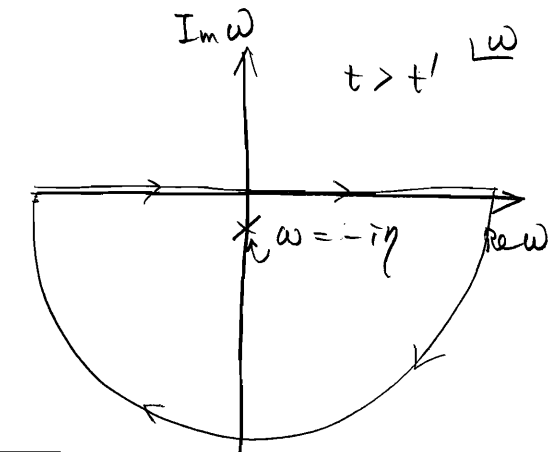
\includegraphics[width = 7cm]{P171.png}
\end{center}
Since the contour encompasses a pole at $\omega=-\mathrm{i}\eta$ in the clockwise way, the integral gives $-2\pi\mathrm{i}$ when $t<t'$, we can put a contour in the upper-half $\omega$-plane, so that the integral here vanishes in the limit of large $|\omega|$, This contour integral doesn't encompass any pole, so that the integral fives zero.

%pic at P172
\begin{center}
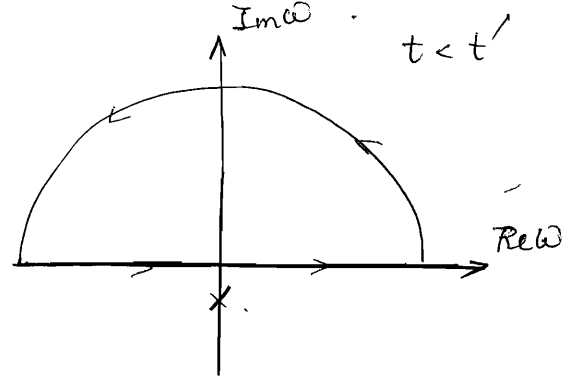
\includegraphics[width = 8cm]{P172.png}
\end{center}
Using this integral representation, the non-interacting fermion green's function can be further calculated as.  
\begin{align}\label{2.3.6}
G^0_{\alpha\beta}(x,t;x',t')&=\frac{1}{2\pi V}\sum_k \int_{-\infty}^{\infty} \mathrm{d}\omega e^{\mathrm{i}k(x-x')-\mathrm{i}\omega_{k}(t-t')} \nonumber \\
& \times \delta_{\alpha\beta}[\frac{\theta(|k|-k_F)}{\omega-\omega_k+\mathrm{i}\eta}+\frac{\theta(k_F-|k|)}{\omega-\omega_k-\mathrm{i}\eta}] \nonumber \\
&\equiv \frac{1}{2\pi V}\sum_k \int_{-\infty}^{\infty}\mathrm{d}\omega e^{\mathrm{i}k(x-x')-\mathrm{i}\omega_{k}(t-t')} G_{\alpha\beta}(k,\omega) \nonumber \\
G_{\alpha\beta}(k,\omega)&\equiv \delta_{\alpha\beta}[\frac{\theta(|k|-k_F)}{\omega-\omega_k+\mathrm{i}\eta}+\frac{\theta(k_F-|k|)}{\omega-\omega_k-\mathrm{i}\eta}] 
\end{align}

To demonstrate how the green's function gives information about the excitation spectrum of the system, let us insert a complete set of eigenstates of H between the two field operators.
\begin{align}\label{2.3.7}
\mathrm{i}G^0_{\alpha\beta}(x,t;x',t')&=\frac{\langle\Psi_0|\mathrm{T}[\hat \psi^{
\dagger}_{H,\alpha}(x,t)\hat \psi_{H,\beta} (x',t')]|\Psi_0\rangle}{\langle\Psi_0|\Psi_0\rangle} \nonumber \\
&=\theta(t-t')\langle\Psi_0|\hat \psi_{H,\alpha}(x,t)\hat{I}\hat \psi^{
\dagger}_{H,\beta} (x',t')|\Psi_0\rangle \nonumber \\
& \ \ \ -\theta(t'-t)\langle\Psi_0|\hat \psi^{
\dagger}_{H,\beta}(x',t')\hat{I}\hat \psi_{H,\alpha} (x,t)|\Psi_0\rangle \nonumber \\
&=\sum_n\{\theta(t-t')\langle\Psi_0|\hat \psi_{H,\alpha}(x,t)|\Psi_n\rangle\times\langle\Psi_n|\hat \psi^{
\dagger}_{H,\beta} (x',t')|\Psi_0\rangle \nonumber \\
& \ \ \ -\theta(t'-t)\langle\Psi_0|\hat \psi^{
\dagger}_{H,\beta}(x',t')|\Psi_n\rangle\times\langle\Psi_n|\hat \psi_{H,\alpha} (x,t)|\Psi_0\rangle\}
\end{align}

Here we assume that the g.s. wave function $|\Psi_0\rangle$ is normalized. And we consider only fermions for simplicity.

By making the time dependence explicit, we can further calculate this as follows

\begin{align}
&=\sum_n\{\theta(t-t')e^{-\mathrm{i}(E_n-E)(t)/\hbar}\langle\Psi_0|\hat \psi_{\alpha}(x)|\Psi_n\rangle\times\langle\Psi_n|\hat \psi^{
\dagger}_{\beta} (x')|\Psi_0\rangle \nonumber \\
& \ \ \ -\theta(t'-t)e^{\mathrm{i}(E_n-E)(t-t')/\hbar}\langle\Psi_0|\hat \psi^{
\dagger}_{\beta}(x')|\Psi_n\rangle\times\langle\Psi_n|\hat \psi_{\alpha} (x)|\Psi_0\rangle\} \nonumber
\end{align}
Note that the states $|\Psi_n\rangle$ here contains N+1 particles if $|\Psi_0\rangle$ contain N particles, while $|\Psi_n\rangle$ here contain N-1 particles.

Now let us assume that the system considered has a translational invariance.

The translational invariance means that the Hamiltonian commute with the total momentum operator $\hat{P}$
\begin{equation}
[\hat{H},\hat{P}]=0\label{2.3.8}
\end{equation}
Where the total momentum operator $\hat{P}$ was already defined in eq(1.4.11) with boson case. But, at this time they are fermion fields.
\begin{equation}
\hat{P}\equiv \sum_{k,\lambda} \hbar k a^k_{k,\lambda} a_{k,\lambda} \nonumber
\end{equation}

Irrespective of this difference, this operator is a generator of the translation.
\begin{equation}\label{2.3.9}
\psi_{\alpha}(x+y)=e^{-\mathrm{i}\hat{P}\cdot y/\hbar}\psi_{\alpha}(x)e^{\mathrm{i}\hat{P}\cdot y/\hbar}
\end{equation}
which can be shown in the same way as we did in eq.(1.4.11).

The translational invariance of the Hamiltonian means that 
\begin{equation}\label{2.3.10}
e^{-\mathrm{i}\hat{P}\cdot y/\hbar}\hat{H}e^{\mathrm{i}\hat{P}\cdot y/\hbar}=\hat{H}
\end{equation}
for any y.

When we use eq.\eqref{2.3.3} for $\hat{H}$, this identity means.

\begin{align}
&\sum_{\alpha}\int \mathrm{d}^3x \hat{\psi^{\dagger}_{\alpha}}(x+y)T(x)\hat{\psi_{\alpha}}(x+y)\nonumber \\
&+\frac{1}{2}\sum_{\alpha,\alpha',\beta,\beta'}\int\mathrm{d}^3x\int\mathrm{d}^3x'\psi^{\dagger}_{\alpha}(x+y)\psi^{\dagger}_{\beta}(x'+y)V_{\alpha\alpha',\beta\beta'}(x,x')\psi^{\dagger}_{\beta'}(x'+y)\psi^{\dagger}_{\alpha}(x+y) \nonumber \\
&=\sum_{\alpha}\int \mathrm{d}^3x \hat{\psi^{\dagger}_{\alpha}}(x)T(x)\hat{\psi_{\alpha}}(x)\nonumber \\
&+\frac{1}{2}\sum_{\alpha,\alpha',\beta,\beta'}\int\mathrm{d}^3x\int\mathrm{d}^3x'\psi^{\dagger}_{\alpha}(x)\psi^{\dagger}_{\beta}(x')V_{\alpha\alpha',\beta\beta'}(x,x')\psi^{\dagger}_{\beta'}(x')\psi^{\dagger}_{\alpha}(x) \nonumber
\end{align}
which clearly represents the translation invariance of the system.

When expanding eq.\eqref{2.3.10} in y, we have, 
\begin{equation}
\hat{H}-\mathrm{i}\frac{1}{\hbar}[\hat{P}\cdot y,\hat{H}]+O(y^2)=\hat{H} \nonumber
\end{equation}
for any y.

which gives us eq.\eqref{2.3.8}

Now that the Hamiltonian commute with the total momentum operator, any eigenstate of $\hat{H}$ should be also eigenstate of $\hat{P}$.

\begin{equation}\label{2.3.11}
\hat{P}|\Psi_n\rangle=P_n|\Psi_n\rangle
\end{equation}

Then, using eq.\eqref{2.3.9} \& eq.\eqref{2.3.11}, we can also extract the x-dependence of eq.\eqref{2.3.7}
\begin{align}
&\mathrm{i}G^0_{\alpha\beta}(x,t;x',t') \nonumber \\
&=\sum_n\bigg [\theta(t-t')e^{-\mathrm{i}(E_n-E)(t)/\hbar}e^{\mathrm{i}\hat{P_n}(x-x')/\hbar}\langle\Psi_0|\hat \psi_{\alpha}(0)|\Psi_n\rangle\times\langle\Psi_n|\hat \psi^{
\dagger}_{\beta} (0)|\Psi_0\rangle \nonumber \\
& \ \ \ -\theta(t'-t)e^{\mathrm{i}(E_n-E)(t-t')/\hbar}e^{-\mathrm{i}\hat{P_n}(x-x')}\langle\Psi_0|\hat \psi^{
\dagger}_{\beta}(0)|\Psi_n\rangle\times\langle\Psi_n|\hat \psi_{\alpha} (0)|\Psi_0\rangle \bigg ] \nonumber
\end{align}
Here we assume that the ground state wave function has zero total momentum.

\begin{equation}
\hat{P}|\Psi_0\rangle=0 \nonumber
\end{equation}
which is usually the case.

Then the Fourier transform of the green's function is given by
\begin{align}
G_{\alpha\beta}(k,\omega)&\equiv\int \mathrm{d}^3(x-x')\int \mathrm{d}^3(t-t')e^{-\mathrm{i}k(x-x')+\mathrm{i}\omega(t-t')}G_{\alpha\beta}(x,t;x',t') \nonumber \\
&=V\sum_n \delta_{k,\hat P_n/\hbar} \frac{\langle\Psi_0|\hat \psi_{\alpha}(0)|\Psi_n\rangle\times\langle\Psi_n|\hat \psi^{
\dagger}_{\beta} (0)|\Psi_0\rangle}{\omega-(E_n-E)/\hbar +\mathrm{i}\eta}  \nonumber \\
&+V\sum_n \delta_{k,-\hat P_n/\hbar} \frac{\langle\Psi_0|\hat \psi^{
\dagger}_{\beta} (0)|\Psi_n\rangle\times\langle\Psi_n|\hat \psi_{\alpha}(0)|\Psi_0\rangle}{\omega+(E_n-E)/\hbar -\mathrm{i}\eta}  \nonumber
\end{align}

This restricts the state $|\Psi_n\rangle$ to have a wave number k, so that we can rewrite this as
\begin{align}
& G_{\alpha\beta}(k,\omega) \nonumber \\
&=V\sum_n \delta_{k,\hat P_n/\hbar} \frac{\langle\Psi_0|\hat \psi_{\alpha}(0)|n,k\rangle\langle n,k|\hat \psi^{
\dagger}_{\beta} (0)|\Psi_0\rangle}{\omega-(E_n-E)/\hbar +\mathrm{i}\eta}  \nonumber \\
&+V\sum_n \delta_{k,-\hat P_n/\hbar} \frac{\langle\Psi_0|\hat \psi^{
\dagger}_{\beta} (0)|n,-k\rangle\langle n,-k|\hat \psi_{\alpha}(0)|\Psi_0\rangle}{\omega+(E_n-E)/\hbar -\mathrm{i}\eta}  \nonumber
\end{align}

In the first sum, the intermediate state has N+1 particles, so that the denominator can be rewritten as
\begin{align}
\omega-[E_n(N+1)-E(N)]/\hbar &= \omega-[E_n(N+1)-E(N+1)]/\hbar-[E(N+1)-E(N)]/\hbar \nonumber \\
&=\omega-\mu/\hbar-\epsilon_n(N+1)/\hbar \nonumber
\end{align}
where $E(N+1)$ and $\epsilon_n(N+1)$ are the ground and the excitation state energy of the (N+1) particle state.

Similarly, the denominator of the second term can be rewritten as 
\begin{align}
\omega+[E_n(N-1)-E(N)]/\hbar &= \omega+[E_n(N-1)-E(N-1)]/\hbar-[E(N)-E(N-1)]/\hbar \nonumber \\
&=\omega-\mu/\hbar+\epsilon_n(N-1)/\hbar \nonumber
\end{align}

Where, in the thermodynamics limit the difference between the former chemical potential and the latter one is negligible.
\begin{align}
E(N+1)-E(N)-(E(n)-E(n-1))=O(N^{-1}) \nonumber \\
\bigg ( Ve(n+\frac{1}{V}) = Ve(n)+ V\frac{\partial e}{\partial n}\frac{1}{V} + \frac{1}{2} \frac{\partial^2 e}{\partial n^2} (\frac{1}{V})^2 \bigg) \nonumber
\end{align}

Using these two, we now obtain 
\begin{align}\label{2.3.12}
& G_{\alpha\beta}(k,\omega) \nonumber \\
&=\hbar V\sum_n \frac{\langle\Psi_0|\hat \psi_{\alpha}(0)|n,k\rangle\langle n,k|\hat \psi^{
\dagger}_{\beta} (0)|\Psi_0\rangle}{\omega\hbar-\mu-\epsilon_n(N+1)+\mathrm{i}\eta}  \nonumber \\
&+\hbar V\sum_n \frac{\langle\Psi_0|\hat \psi^{
\dagger}_{\beta} (0)|n,-k\rangle\langle n,-k|\hat \psi_{\alpha}(0)|\Psi_0\rangle}{\omega\hbar-\mu+\epsilon_n(N-1)-\mathrm{i}\eta} 
\end{align}

This representation of single-particle green's function is called as Lehmann representation.

If the Hamiltonian and the ground state are invariant under the spatial rotation and reflection, the green's function has a following matrix structure.
\begin{equation}
G_{\alpha\beta}=\delta_{\alpha\beta}G(|k|,\omega) \nonumber
\end{equation}

The lehmann rep. exhibits the $\omega$-dependence of the exact green's function of interacting systems.

The function $G(k,\omega)$ is a meromorphic function of $\omega$, with simple poles at the exact excitation energy of the interacting system corresponding to a momentum $\hbar k$.

For frequencies below $\mu/\hbar$, these singularities lies slightly above the real axis and for frequencies above $\mu/\hbar$, these singularities  lies slightly below the real axis.

%pic at P184
\begin{center}
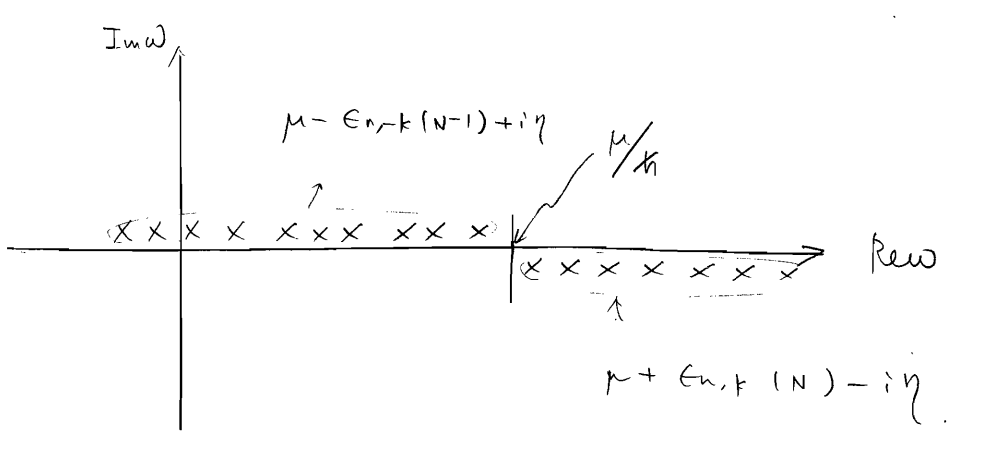
\includegraphics[width = 10cm]{P184.png}
\end{center}
In this way, the singularities if the green's function yield the energies of those excited states for which the numerator ($\langle n,k|\hat \psi^{
\dagger}_{\beta} (0)|\Psi_0\rangle$ or $\langle n,-k|\hat \psi_{\alpha}(0)|\Psi_0\rangle$) does not vanish. 

For the non-interacting system, this representation reproduce eq.eq.\eqref{2.3.6}.

\begin{equation}
G^0(k,\omega)=\frac{\theta(k-k_F)}{\omega-\omega_k+\mathrm{i}\eta}+\frac{\theta(k_F-k)}{\omega-\omega_k-\mathrm{i}\eta} \nonumber
\end{equation} 
with $\omega_k=\frac{\hbar^2k^2}{2m}$

Namely, for the non-interacting system, the field operator connects only one state to the ground state, so that $G^0(k,\omega)$ has only a single pole, slightly below the real axis at $\hbar \omega=\frac{\hbar^2k^2}{2m}$ if $k>k_F$ and slightly above the real axis at the same value of $\hbar \omega$ of $k<k_F$.


% pic at P185
\begin{center}
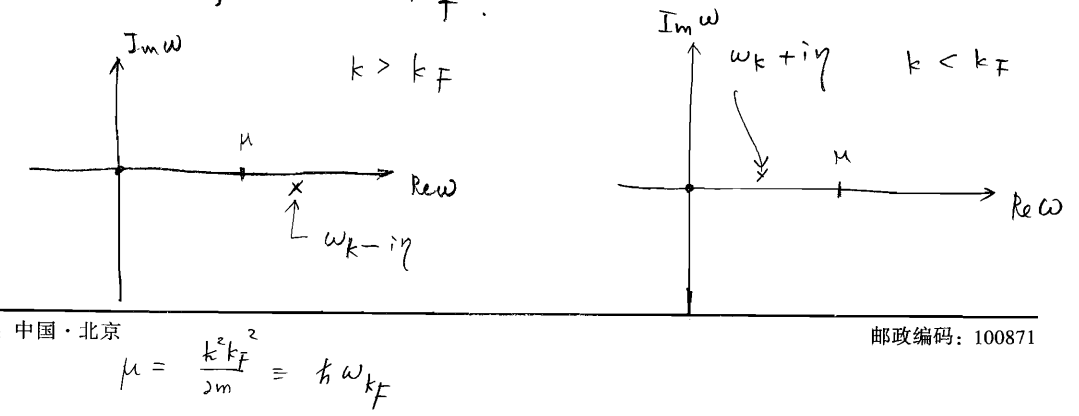
\includegraphics[width = 12cm]{P185.png}
\end{center}

The green's function is analytic in neither the upper $\omega$-plane nor the lower $\omega$-plane.

We define a new pair of function, known as retard and advance green's functions.
\begin{align}\label{2.3.13}
\mathrm{i}G^R_{\alpha\beta}(x,t;x',t')=\langle \Psi_0|\{\hat \psi_{H,\alpha}(x,t),\psi^{\dagger}_{H,\beta}(x',t')\}|\Psi_0\rangle\theta(t-t')
\end{align}
\begin{align}\label{2.3.14}
\mathrm{i}G^A_{\alpha\beta}(x,t;x',t')=\langle \Psi_0|\{\hat \psi_{H,\alpha}(x,t),\psi^{\dagger}_{H,\beta}(x',t')\}|\Psi_0\rangle\theta(t'-t)
\end{align}
with $\{A,B\}\equiv AB+BA$

Using the exactly same analysis, we can show the following Lehmann representation of their Fourier transforms.

\begin{align}\label{2.3.15}
& G^{R/A}_{\alpha\beta}(k,\omega) \nonumber \\
&=\hbar V\sum_n \frac{\langle\Psi_0|\hat \psi_{\alpha}(0)|n,k\rangle\langle n,k|\hat \psi^{
\dagger}_{\beta} (0)|\Psi_0\rangle}{\omega\hbar-\mu-\epsilon_n(N+1)\pm\mathrm{i}\eta}  \nonumber \\
&+\hbar V\sum_n \frac{\langle\Psi_0|\hat \psi^{
\dagger}_{\beta} (0)|n,-k\rangle\langle n,-k|\hat \psi_{\alpha}(0)|\Psi_0\rangle}{\omega\hbar-\mu+\epsilon_n(N-1)\pm\mathrm{i}\eta} \nonumber\tag{2.3.15A/B} 
\end{align}

Note that all the poles of $G^R$ lie in the lower half plane, so that $G^A(k,\omega)$ is analytic for $\mathrm{Im} \omega<0$



\section{Wick's theorem}

So far, we define the single-particle green's function and show its relation to physical observables.

To evaluate the green's function for nontrivial physical systems, we use perturbation theory.

This procedure is mostly carried out in the interacting picture, instead of the Heinsenberg picture.

Let me first prove a basic Theorem that relates the matrix elements of Heisenberg operators to the matrix elements of the corresponding interaction operators.


\begin{align}\label{2.4.1}
\frac{\langle\Psi_0|\hat{O_H}(t)|\Psi_0\rangle}{\langle\Psi_0|\Psi_0\rangle}=\frac{1}{\langle\Phi_0|\hat{S}|\Phi_0\rangle}\times \langle\Phi_0|\sum_{\nu=0}^{\infty}(\frac{-\mathrm{i}}{\hbar})^{\nu} \frac{1}{\nu!} \int_{-\infty}^{+\infty}\mathrm{d}t_1......\int_{-\infty}^{+\infty}\mathrm{d}t_{\nu} \nonumber \\
e^{-\epsilon(|t_1|+...+|t_{\nu}|)}\mathrm{T}[\hat{H_1}(t_1)...\hat{H_1}(t_{\nu})]\hat{O_I}(t)|\Phi_0\rangle
\end{align}
where 
\begin{equation}\label{2.4.2}
\hat{S}\equiv\hat{U_{\epsilon}}(\infty,-\infty)
\end{equation}

The proof is as follows.

According to the Gell-Mann \& Low Theorem, $|\Psi_0\rangle$ can be given by

\begin{align}
\frac{|\Psi_0\rangle}{\langle\Phi_0|\Psi_0\rangle}&=\frac{\hat{U_{\epsilon}}(+\infty,0)|\Psi_0\rangle}{\langle\Phi_0|\hat U_{\epsilon}(+\infty,0)|\Psi_0\rangle} \nonumber \\
&=\frac{\hat{U_{\epsilon}}(0,-\infty)|\Psi_0\rangle}{\langle\Phi_0|\hat U_{\epsilon}(0,-\infty)|\Psi_0\rangle} \nonumber
\end{align}

By taking an inner product between these two, we can calculate this part
\begin{align}
\frac{\langle\Psi_0|\Psi_0\rangle}{|\langle\Phi_0|\Psi_0\rangle|^2}&=\frac{\langle\Phi_0|\hat{U_{\epsilon}}(+\infty,0)\hat{U_{\epsilon}}(0,-\infty)|\Phi_0\rangle}{\langle\Phi_0|\hat{U^{\dagger}_{\epsilon}}(+\infty,0)|\Phi_0\rangle^*\langle\Phi_0|\hat{U_{\epsilon}}(0,-\infty)|\Phi_0\rangle} \nonumber \\
&=\frac{\langle\Phi_0|\hat{U_{\epsilon}}(+\infty,0)\hat{U_{\epsilon}}(0,-\infty)|\Phi_0\rangle}{D} \nonumber \\
&= \frac{\langle\Phi_0|\hat{U_{\epsilon}}(+\infty,-\infty)|\Phi_0\rangle}{D} \nonumber
\end{align}
The numerator can be also calculated in a similar way.
\begin{align}
\frac{\langle\Psi_0|\hat{O_H}(t)|\Psi_0\rangle}{|\langle\Phi_0|\Psi_0\rangle|^2}&=\frac{\langle\Phi_0|\hat{U_{\epsilon}}(+\infty,0)\hat{O_H}(t)\hat{U_{\epsilon}}(0,-\infty)|\Phi_0\rangle}{\langle\Phi_0|\hat{U^{\dagger}_{\epsilon}}(+\infty,0)|\Phi_0\rangle^*\langle\Phi_0|\hat{U_{\epsilon}}(0,-\infty)|\Phi_0\rangle} \nonumber \\
&=\frac{\langle\Phi_0|\hat{U_{\epsilon}}(+\infty,0)\hat{U_{\epsilon}}(0,t)\hat{O_I}(t)\hat{U_{\epsilon}}(t,0)\hat{U_{\epsilon}}(0,-\infty)|\Phi_0\rangle}{D} \nonumber \\
&=\frac{\langle\Phi_0|\hat{U_{\epsilon}}(+\infty,t)\hat{O_I}(t)\hat{U_{\epsilon}}(t,-\infty)|\Phi_0\rangle}{D} \nonumber
\end{align}


Now that these two equations share the same denominator, we can make them cancel each other so as to obtain
\begin{align}
\frac{\langle\Psi_0|\hat{O_H}(t)|\Psi_0\rangle}{\langle\Psi_0|\Psi_0\rangle}=\frac{\langle\Phi_0|\hat{U_{\epsilon}}(+\infty,t)\hat{O_I}(t)\hat{U_{\epsilon}}(t,-\infty)|\Phi_0\rangle}{\langle\Phi_0|\hat{U_{\epsilon}}(+\infty,-\infty)|\Phi_0\rangle}\nonumber
\end{align}

The numerator  of the r.h.s is given as
\begin{align}
\hat{U_{\epsilon}}(+\infty,t)\hat{O_I}(t)\hat{U_{\epsilon}}(t,-\infty)=&\sum_{n=0}^{\infty}(\frac{-\mathrm{i}}{\hbar})^{n} \frac{1}{n!} \int_{-\infty}^{+\infty}\mathrm{d}t_1......\int_{-\infty}^{+\infty}\mathrm{d}t_{n} \nonumber \\
& \times e^{-\epsilon(|t_1|+...+|t_{n}|)}\mathrm{T}[\hat{H_1}(t_1)...\hat{H_1}(t_{n})]\hat{O_I}(t)\times \nonumber \\
& \sum_{m=0}^{\infty}(\frac{-\mathrm{i}}{\hbar})^{m} \frac{1}{m!} \int_{-\infty}^{+\infty}\mathrm{d}s_1......\int_{-\infty}^{+\infty}\mathrm{d}s_{m} \nonumber \\
& \times e^{-\epsilon(|s_1|+...+|s_{m}|)}\mathrm{T}[\hat{H_1}(s_1)...\hat{H_1}(s_{m})]\times \nonumber \\
& ...... \nonumber
\end{align}

On the one hand, the numerator of eq.\eqref{2.4.1} can be rewritten as follows.

Firstly, suppose that we divide  $\nu$-numbers of $\hat{H_1}$ into n-numbers of $\hat{H_1}$ whose times one greater than 't' and ($\nu$-n)-numbers of $\hat{H_1}$ whose times are less than 't',
\begin{align}
=\sum_{\nu=0}^{\infty}(\frac{-\mathrm{i}}{\hbar})^{\nu} \frac{1}{\nu!} \sum_{n=0}^{\nu}\frac{\nu!}{n!(\nu-n)!}e^{-\epsilon(|t_1|+...+|t_{\nu}|)} \int_{t}^{+\infty}\mathrm{d}t_1...\int_{t}^{+\infty}\mathrm{d}t_{n} 
\int_{-\infty}^{t}\mathrm{d}t_{n+1}...\int_{-\infty}^{t}\mathrm{d}t_{\nu} \nonumber \\
\mathrm{T}[\hat{H_1}(t_1)...\hat{H_1}(t_{n})]\hat{O_I}(t)\mathrm{T}[\hat{H_1}(t_{n+1})...\hat{H_1}(t_{\nu})] \nonumber
\end{align}

There is $\frac{\nu!}{n!(\nu-n)!}$ number of (the factorial of $\nu$ divided by the factorial of n times the factorial of ($\nu-n$)) ways of dividing.

Thus, once we choose $t_1,t_2,...,t_n$ to be greater than t while the  remaining to be less than t, we need to multiply this factor.

Since 
\begin{equation}
\sum_{\nu=0}^{+\infty}\sum_{n=0}^{\nu} f_{n,\nu}=\sum_{m=0}^{+\infty}\sum_{n=0}^{\nu} f_{n,m+n} \nonumber
\end{equation}
%pic at194
\begin{center}
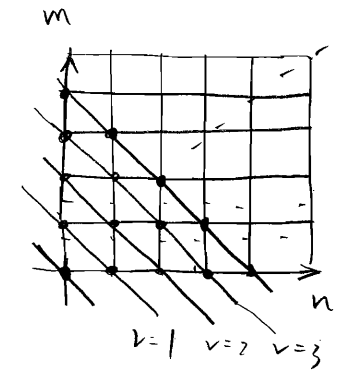
\includegraphics[width = 4cm]{P194.png}
\end{center}
So that
\begin{align}
=&\sum_{m=0}^{+\infty}\frac{1}{m!}(\frac{-\mathrm{i}}{\hbar})^m\sum_{n=0}^{+\infty} \frac{1}{n!}(\frac{-\mathrm{i}}{\hbar})^ne^{-\epsilon(|t_1|+...+|t_{m+n}|)} \nonumber \\
&\int_{t}^{+\infty}\mathrm{d}t_1...\int_{t}^{+\infty}\mathrm{d}t_n\int_{-\infty}^{t}\mathrm{d}t_{n+1}...\int_{-\infty}^{t}\mathrm{d}t_{n+m} \nonumber \\
&\mathrm{T}[\hat{H_1}(t_1)...\hat{H_1}(t_n)]\hat{O_I}(t)\mathrm{T}[\hat{H_1}(t_{n+1})...\hat{H_1}(t_{n+m})] \nonumber \\
=& \hat U_{\epsilon}(-\infty,t)\hat{O_I}(t)\hat U_{\epsilon}(t,-\infty) \nonumber
\end{align}

This proves eq.\eqref{2.4.1}

In a similar way, we can show that  the expectation value of time-ordered Heinsenberg operator can be expressed in terms of the interaction picture.
\begin{align}\label{2.4.3}
\frac{\langle\Psi_0|\mathrm{T}[\hat{O_H}(t)\hat{O_H}(t')]|\Psi_0\rangle}{\langle\Psi_0|\Psi_0\rangle}=&\frac{1}{\langle\Phi_0|\hat{S}|\Phi_0\rangle}\times\langle\Phi_0|\sum_{\nu=0}^{\infty}(\frac{-\mathrm{i}}{\hbar})^{\nu} \frac{1}{\nu!} \int_{-\infty}^{+\infty}\mathrm{d}t_1......\int_{-\infty}^{+\infty}\mathrm{d}t_{\nu}e^{-\epsilon(|t_1|+...+|t_{\nu}|)} \nonumber\\
&\times \mathrm{T}[\hat{H_1}(t_1)...\hat{H_1}(t_{\nu})\hat{O_I}(t)\hat{O_I}(t')]|\Phi_0\rangle
\end{align}
The r.h.s reads.
\begin{align}
&\frac{\langle\Psi_0|\mathrm{T}[\hat O_{H}(t)\hat O_H (t')]|\Psi_0\rangle}{\langle\Psi_0|\Psi_0\rangle} \nonumber \\
=&\theta(t-t')\langle\Psi_0|\hat O_{H}(t)\hat O_H (t')|\Psi_0\rangle \nonumber \\
& \ \ +\theta(t'-t)\langle\Psi_0|\hat O_{H}(t')\hat O_H (t)|\Psi_0\rangle \nonumber 
\end{align}
The numerator of the first term can be calculated in the same way as before,
\begin{align}
\frac{\langle\Psi_0|\hat{O_H}(t)\hat{O_H}(t')|\Psi_0\rangle}{|\langle\Phi_0|\Psi_0\rangle|^2}&=\frac{\langle\Phi_0|\hat{U_{\epsilon}}(+\infty,0)\hat{O_H}(t)\hat{O_H}(t')\hat{U_{\epsilon}}(0,-\infty)|\Phi_0\rangle}{D} \nonumber \\
&=\frac{\langle\Phi_0|\hat{U_{\epsilon}}(+\infty,t)\hat{O_I}(t)\hat{U_{\epsilon}}(t,t')\hat{O_I}(t')\hat{U_{\epsilon}}(t',-\infty)|\Phi_0\rangle}{D} \nonumber
\end{align}
So that, we can employ the same cancellation between D which comes from the numerator and D which comes from the denominator.
\begin{align}
\frac{\langle\Psi_0|\hat{O_H}(t)\hat{O_H}(t')|\Psi_0\rangle}{\langle\Psi_0|\Psi_0\rangle}=\frac{\langle\Phi_0|\hat{U_{\epsilon}}(+\infty,t)\hat{O_I}(t)\hat{U_{\epsilon}}(t,t')\hat{O_I}(t')\hat{U_{\epsilon}}(t',-\infty)|\Phi_0\rangle}{\langle\Phi_0|\hat{U_{\epsilon}}(+\infty,-\infty)|\Phi_0\rangle}\nonumber
\end{align}
for $t'>t$

On the one hand, the numerator of the r.h.s of eq.\eqref{2.4.3} can be calculated as
\begin{align}
(r.h.s)=\theta&(t-t')\langle \Phi_0|\sum_{\nu=0}^{\infty}(\frac{-\mathrm{i}}{\hbar})^{\nu} \frac{1}{\nu!}\sum_{n}\sum_{m}^{0<n+m\le\nu}\frac{\nu!}{n!m!(\nu-n-m)!}\nonumber\\ &\int_{t}^{+\infty}\mathrm{d}t_1...\int_{t}^{+\infty}\mathrm{d}t_{n}\int_{t'}^{t}\mathrm{d}t_{n+1}...\int_{t'}^{t}\mathrm{d}t_{n+m}\int_{-\infty}^{t'}\mathrm{d}t_{n+m+1}...\int_{-\infty}^{t'}\mathrm{d}t_{\nu} \nonumber \\
\times&  \mathrm{T}[\hat{H_1}(t_1)...\hat{H_1}(t_{n})]\hat{O_I}(t)\mathrm{T}[\hat{H_1}(t_{n+1})...\hat{H_1}(t_{n+m})]\hat{O_I}(t')\mathrm{T}[\hat{H_1}(t_{n+m+1})...\hat{H_1}(t_{\nu})]|\Phi_0\rangle \nonumber \\
+&\theta(t'-t)\langle \Phi_0|\sum_{\nu=0}^{\infty}(\frac{-\mathrm{i}}{\hbar})^{\nu} \frac{1}{\nu!}\sum_{n}\sum_{m}^{0\le n+m\le\nu}\frac{\nu!}{n!m!(\nu-n-m)!}\nonumber\\ &\int_{t'}^{+\infty}\mathrm{d}t_1...\int_{t'}^{+\infty}\mathrm{d}t_{n}\int_{t}^{t'}\mathrm{d}t_{n+1}...\int_{t}^{t'}\mathrm{d}t_{n+m}\int_{-\infty}^{t}\mathrm{d}t_{n+m+1}...\int_{-\infty}^{t}\mathrm{d}t_{\nu} \nonumber \\
\times&  \mathrm{T}[\hat{H_1}(t_1)...\hat{H_1}(t_{n})]\hat{O_I}(t')\mathrm{T}[\hat{H_1}(t_{n+1})...\hat{H_1}(t_{n+m})]\hat{O_I}(t)\mathrm{T}[\hat{H_1}(t_{n+m+1})...\hat{H_1}(t_{\nu})]|\Phi_0\rangle \nonumber
\end{align}
This part can be replaced by this
\begin{align}
&\sum_{\nu=0}^{\infty}\sum_{n}\sum_{m}^{0<n+m\le\nu}\frac{1}{n!m!(\nu-n-m)!}\nonumber\\
=&\sum_{n=0}^{\infty}\sum_{m=0}^{\infty}\sum_{l=0}^{\infty}\frac{1}{n!m!l!} \nonumber
\end{align}
%pic at199
\begin{center}
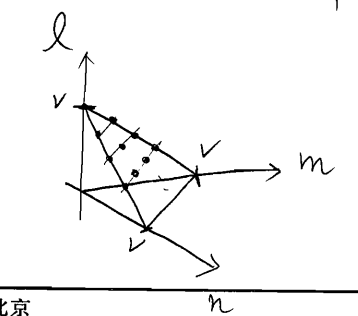
\includegraphics[width = 3cm]{P199.png}
\end{center}
So that the first term reduces to
\begin{align}
(1st \  term)=\theta(t-t')\langle\Phi_0|\hat{U_{\epsilon}}(+\infty,t)\hat{O_I}(t)\hat{U_{\epsilon}}(t,t')\hat{O_I}(t')\hat{U_{\epsilon}}(t',-\infty)|\Phi_0\rangle \nonumber
\end{align}
while the 2nd term reduces to
\begin{align}
(2nd \  term)=\theta(t'-t)\langle\Phi_0|\hat{U_{\epsilon}}(+\infty,t')\hat{O_I}(t')\hat{U_{\epsilon}}(t',t)\hat{O_I}(t)\hat{U_{\epsilon}}(t,-\infty)|\Phi_0\rangle \nonumber
\end{align}
which proves eq.\eqref{2.4.3}

These two formula are among the most useful results of quantum field theory.


Armed with these formulas, let us consider the  single-particle green's function, which is now given in the interaction picture.
\begin{align}\label{2.4.4}
\mathrm{i}G_{\alpha\beta}(x,t;x',t')=\sum_{\nu=0}^{\infty}(\frac{-\mathrm{i}}{\hbar})^{\nu} \frac{1}{\nu!} \int_{-\infty}^{+\infty}\mathrm{d}t_1......\int_{-\infty}^{+\infty}\mathrm{d}t_{\nu}\times\nonumber  \\
\frac{\langle\Phi_0|\mathrm{T[\hat H_1(t_1)...\hat H_1(t_{\nu})\hat \Psi_{I,\alpha}(x)\Psi^{\dagger}_{I,\beta}(x')]}
|\Phi_0\rangle}{\langle\Phi_0|\hat{U_{\epsilon}}(+\infty,-\infty)|\Phi_0\rangle}
\end{align}
where $x\ \&\ x'$ here denotes space and temporal coordinate.$x\equiv(x,t),x\equiv (x',t')$
\begin{align}
\Psi_{I,\alpha}(x)&\equiv\Psi_{I,\alpha}(x,t) \nonumber \\
&=e^{\mathrm{i}\hat{H_0}t/\hbar}\Psi_{\alpha}(x)e^{-\mathrm{i}\hat{H_0}t/\hbar} \nonumber
\end{align}
This operator is now creation and annihilation operator in the interaction picture.

For Hamiltonian defined in eq.\eqref{2.3.3}, the numerator of this eq. becomes as follows:

numerator of eq.\eqref{2.4.4}
\begin{align}\label{2.4.5}
& numerator of eq.\eqref{2.4.4} \nonumber \\
=&\langle \Phi_0|\mathrm{T}[\hat \psi_{\alpha }(x)\hat \psi_{\beta }^{\dagger}(x')]|\Phi\rangle \nonumber \\
&+(\frac{-\mathrm{i}}{\hbar})\sum_{\lambda,\lambda',\mu,\mu'}\frac{1}{2}\int_{-\infty}^{+\infty}\mathrm{d}t_1\int\mathrm{d}^3x_1\int\mathrm{d}^3x_1' \nonumber \\
&\times U_{\lambda\lambda',\mu\mu'}(x_1,x_1')\times \nonumber\\
&\Phi_0|\mathrm{T}[\hat \psi_{I,\lambda}^{\dagger}(x_1,t_1)\hat \psi_{I,\mu}^{\dagger}(x_1',t_1)\hat \psi_{I,\mu' }(x_1',t_1) \nonumber \\
&\ \ \ \hat \psi_{I,\lambda' }(x_1,t_1)\hat \psi_{I,\alpha}(x,t)\hat \psi^{\dagger}_{I,\beta }(x',t)]|\Phi\rangle \nonumber \\
&\ \ \ \ \ +......
\end{align}
This expression shows that, we must evaluate the expectation value in the non-interacting ground state of T-products of creation \& destruction operators of the form:
\begin{align}
\Phi_0|\mathrm{T}[\hat \psi_{I}^{\dagger}......\hat \psi_{I}\hat \psi_{I,\alpha}(x)\hat \psi^{\dagger}_{I,\beta }(x')]|\Phi\rangle \nonumber 
\end{align}
To evaluate this form of quantities, we will rely on so-called Wick's theorem, which I will explain next.

The essential ideas of Wick's theorem is to move all destruction operators to the right, where they annihilate the non-interacting ground state wave function.

For this purpose, we decompose the field operator into a destruction part (the 1st term in the r.h.s of following equation) that annihilates the non-interacting ground state and a creation part(the 2nd term).
\begin{align}
\hat \psi_{I}(x)=\hat \psi^{(+)}_{I}(x)&+\hat \psi^{(-)}_{I}(x) \nonumber \\
\hat \psi^{(+)}_{I}(x)|\Phi_0\rangle&=0 \nonumber
\end{align}

Note also that any two pairs of destruction operators thus defined commute or anticommute with each other, which can be seen by taking the expectation value of their commutator or anticommutator.

\begin{align}
&\{\hat \psi^{(+)}(x),\hat \psi^{(+)}(y)\}_{\pm}=0 \nonumber \\
\big (&\leftarrow\langle\Phi_0|\hat \psi^{(+)}(x)\hat \psi^{(+)}(y)\pm\hat \psi^{(+)}(y),\hat \psi^{(+)}(x)|\Phi_0\rangle \big) \nonumber \\
&\{\hat \psi^{(-)\dagger}(x),\hat \psi^{(+)}(y)\}_{\pm}=0 \nonumber \\
\big (&\leftarrow\langle\Phi_0|\hat \psi^{(-)\dagger}(x)\hat \psi^{(+)}(y)\pm\hat \psi^{(+)}(y),\hat \psi^{(-)\dagger}(x)|\Phi_0\rangle \big) \nonumber
\end{align} 
+ for fermion case, - for boson case.

Similarly, we can see that any two pairs of creation part commute of anticommute with each other.
\begin{align}
&\{\hat \psi^{(-)}(x),\hat \psi^{(-)}(y)\}_{\pm}=\{\hat \psi^{(-)}(x),\hat \psi^{(+)\dagger}(y)\}_{\pm} \nonumber \\
=&\{\hat \psi^{(+)\dagger}(x),\hat \psi^{(+)\dagger}(y)\}_{\pm}=0 \nonumber 
\end{align}

Correspondingly, we have
\begin{align}
\hat \psi^{\dagger}_{I}(x)=\hat \psi^{(+)\dagger}_{I}(x)&+\hat \psi^{(-)\dagger}_{I}(x) \nonumber \\
\hat \psi^{(-)}_{I}(x)|\Phi_0\rangle&=0 \nonumber
\end{align}
Where we take the adjoint of this, so as to obtain this.

As an explicit example of this decomposition, consider the free fermion field given in eq. H
\begin{align}
\hat \psi_I(x)=\frac{1}{\sqrt{V}}\sum_{k>k_F} e^{\mathrm{i}(kx-\mathrm{i}\omega_kt)}a_k+\frac{1}{\sqrt{V}}\sum_{k<k_F} e^{\mathrm{i}(kx-\mathrm{i}\omega_kt)}a_k \nonumber
\end{align}
Where I have omitted the spin index

This satisfies $\hat \phi^{(-)}(x)|\Phi_0\rangle=\hat \phi ^{(+)}|\Phi_0\rangle=0$, because $|\Phi_0\rangle$ is a Fermi sea state with fermions being occupied up to the fermi level.

$\circledcirc$ As was already defined in eq.\eqref{2.3.2}, time-order products orders the field operators with the latest time om the left
\begin{align}
\mathrm{T}(\hat{A}\hat{B}\hat{C}\hat{D}...)=(-1)^P\hat{B}\hat{D}\hat{C}\hat{A}... \nonumber
\end{align}
with $t_B>t_D>t_C>t_A>...$

Where this factor become +1 if the time ordering is accompanied by the even numbers of interchange of the fermion field.

while this factor become -1 if the time ordering is accompanied by the odd numbers of interchange of the fermion field.

For boson case, this is always +1.

Thus, we can freely reorder the field operators within the F product, in such a way that fermion fields anticommute and boson fields commute.

$\circledcirc$ The other important operator product is the "normal ordering", in which all the annihilation operators are placed to the right of all the creation operators again including a factor -1 for every interchange of fermion operators.
 % pic at P209
 \begin{center}
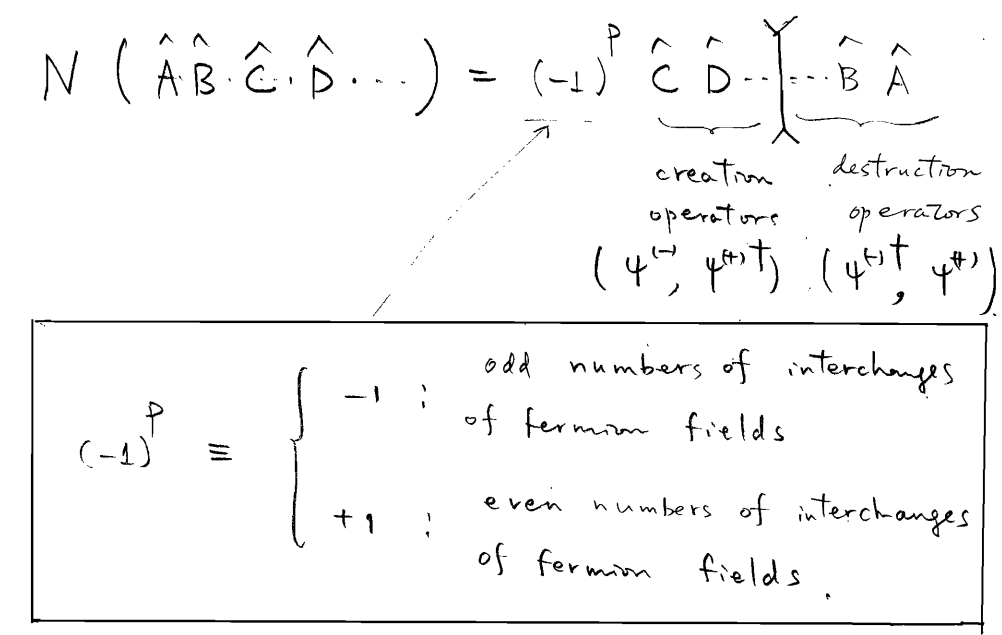
\includegraphics[width = 12cm]{P209.png}
\end{center}
Here the destruction operators means a destruction part of field operator which annihilates the non-interacting groundstate. while the creation operator means a creation part which does not.

Because any two pairs of destruction parts commute or anticommute with each other and also because that is the case for creation parts, the r.h.s of this is uniquely defined.

Namely, a specific order within a set of destruction operators in the right and that with a set of creation operators in the left don't make any difference.

For example, for fermion case, we have 

\begin{align}
\mathrm{N}[\hat \psi^{(+)}(x)\hat \psi^{(-)}(y)]&=-\hat \psi^{(-)}(y)\hat \psi^{(+)}(x) \nonumber \\
\mathrm{N}[\hat \psi^{(-)\dagger}(x)\hat \psi^{(+)\dagger}(y)]&=-\hat \psi^{(+)\dagger}(y)\hat \psi^{(-)\dagger}(x) \nonumber \\
\mathrm{N}[\hat \psi^{(-)\dagger}(x)\hat \psi^{(+)}(y)]&=\hat \psi^{(-)\dagger}(x)\hat \psi^{(+)}(y) \nonumber \\
&=-\hat \psi^{(+)}(y)\hat \psi^{(-)\dagger}(x) \nonumber \\
\mathrm{N}[\hat \psi^{(-)}(x)\hat \psi^{(+)\dagger}(y)]&=\hat \psi^{(-)}(x)\hat \psi^{(+)\dagger}(y) \nonumber \\
&=-\hat \psi^{(+)\dagger}(y)\hat \psi^{(-)}(x) \nonumber 
\end{align}
Here I have omitted the subscript 'I'. I will do so in the remaining part of today's lecture, because the field operators are always in the interaction picture.

A normal order product is very useful, because its expectation value in the non-interacting ground state $|\Phi_0\rangle$ always vanishes.

\begin{align}
&\langle\Psi_0|\mathrm{N}(\hat{A}\hat{B}\hat{C}\hat{D}...)|\Psi_0\rangle \nonumber \\
=&(-1)^P\langle\Psi_0|\mathrm{N}(\hat{C}\hat{D}...||...\hat{A}\hat{B})|\Psi_0\rangle=0 \nonumber
\end{align}
Using this useful feature, we will evaluate the ground-state expectation value of a T product of operators, by reducing the T product into the corresponding Normal ordered product.

Note also that the normal ordering product has a distributive feature

\begin{align}
\mathrm{N}[(\hat{A}+\hat{B})\cdot(\hat{C}+\hat{D})\cdot...]=&\mathrm{N}[\hat{A}\cdot\hat{C}\cdot...]+\mathrm{N}[\hat{A}\cdot\hat{D}\cdot...] \nonumber \\
&+\mathrm{N}[\hat{B}\cdot\hat{C}\cdot...]+\mathrm{N}[\hat{B}\cdot\hat{D}\cdot...] \nonumber
\end{align}

$\circledcirc$ The third item I want to define before describing Wick's theorem is "contractions". 


The contraction are defined between two fermion fields and is equal to the difference between their T-product and their N-product.

\begin{align}
\hat{U^{\cdot}}\hat{V^{\cdot}} \equiv \mathrm{T}(\hat{U}\hat{V})-\mathrm{N}(\hat{U}\hat{V}) \nonumber
\end{align}

This two dot (superscript) marks dictate that these two fields are "contracted".

Most of the  contractions actually are zero.

For example $\hat \psi_{(+)} \ \&\  \hat \psi_{(-)}$ commute or anticommute with each other, so that their time-ordered product and normal-ordered product are same.

\begin{align}
\mathrm{T}[\hat \psi_{(+)}(x)\hat \psi_{(-)}(x')]&=\theta(t-t')\hat \psi_{(+)}(x)\hat \psi_{(-)}(x')\mp \theta(t'-t)\hat \psi_{(-)}(x')\hat \psi_{(+)}(x) \nonumber \\
&=\mp\hat \psi_{(-)}(x')\hat \psi_{(+)}(x) \nonumber \\
&=\mathrm{N}[\hat \psi_{(+)}(x)\hat \psi_{(-)}(x')] \nonumber
\end{align}
As a result, their contraction becomes zero.
\begin{align}
\hat \psi^{\cdot}_{(+)}(x)\hat \psi^{\cdot}_{(-)}(x')=0\nonumber
\end{align}
\begin{align}
&\{\hat \psi^{(+)\dagger}(x),\hat \psi^{(-)\dagger}(y)\}_{\pm}=\{\hat \psi^{(+)\dagger}(x),\hat \psi^{(-)}(y)\}_{\pm} \nonumber \\
=&\{\hat \psi^{(+)}(x),\hat \psi^{(-)\dagger}(y)\}_{\pm}=\{\hat \psi^{(+)}(x),\hat \psi^{(+)}(y)\}_{\pm} \nonumber \\
=&\{\hat \psi^{(-)}(x),\hat \psi^{(-)}(y)\}_{\pm}= 0 \nonumber
\end{align}
Thus, we can also show in the same way that the contractions of these pairs of fermion fields are all zero.
\begin{align}
&\hat \psi^{(+)\dagger\cdot}\hat \psi^{(-)\cdot}=\hat \psi^{(-)\cdot}\hat \psi^{(-)\cdot}=0 \nonumber \\
&\hat \psi^{(+)\cdot}\hat \psi^{(+)\cdot}=\hat \psi^{(-)\cdot}\hat \psi^{(-)\cdot}=\hat \psi^{(+)\cdot}\hat \psi^{(-)\cdot}=0\nonumber \\
&\hat \psi^{(+)\dagger\cdot}\hat \psi^{(+)\dagger\cdot}=\hat \psi^{(-)\dagger\cdot}\hat \psi^{(-)\dagger\cdot}=\hat \psi^{(+)\dagger\cdot}\hat \psi^{(-)\dagger\cdot}=0 \nonumber
\end{align}
Non-zero contractions come from those pairs of fermions which do not commute or anticommute.

$\hat \psi^{(+)\cdot}\hat \psi^{(+)\dagger\cdot},\hat \psi^{(-)\cdot}\hat \psi^{(-)\dagger\cdot}$

first term can be calculated as 
\begin{align}
\hat \psi^{(+)\cdot}(x)\hat \psi^{(+)\dagger\cdot}(x')&=\mathrm{T}[\hat \psi^{(+)\cdot}(x)\hat \psi^{(+)\dagger\cdot}(x')]-\mathrm{N}[\hat \psi^{(+)\cdot}(x)\hat \psi^{(+)\dagger\cdot}(x')] \nonumber \\
&=\theta (t-t')\hat \psi^{(+)\cdot}(x)\hat \psi^{(+)\dagger\cdot}(x')\mp\theta (t'-t)\hat \psi^{(+)\dagger\cdot}(x')\hat \psi^{(+)\cdot}(x)-(\mp)\theta (t'-t)\hat \psi^{(+)\dagger\cdot}(x')\hat \psi^{(+)\cdot}(x) \nonumber \\
&=\theta(t-t')\{\hat \psi^{(+)\cdot}(x),\hat \psi^{(+)\dagger\cdot}(x')\}_{\pm} \nonumber
\end{align}
which remains finite only when $t>t'$.

Moreover the r.h.s is just a c-number instead of operator, because this is a commutator of anticommutator of two field operators in interaction picture.

By taking the expectation value of this eq. with respect to the non-interacting ground state, we can calculate this c-number as

\begin{align}
\hat \psi^{(+)\cdot}(x)\hat \psi^{(+)\dagger\cdot}(x')=\theta(t-t')\langle\Phi_0|\hat \psi^{(+)}(x)\hat \psi^{(+)\dagger}(x')|\Phi_0\rangle \nonumber
\end{align}
Similarly we can show that 
\begin{align}
\hat \psi^{(-)\cdot}(x)\hat \psi^{(-)\dagger\cdot}(x')=\mp\theta(t'-t)\langle\Phi_0|\hat \psi^{(-)\dagger}(x')\hat \psi^{(-)}(x)|\Phi_0\rangle \nonumber
\end{align}
Combining these two and noting the distributive nature of normal-ordering \& time-ordering, we obtain

\begin{align}
\hat{\psi^{\cdot}}(x)\hat{\psi^{\dagger\cdot}}(x')=&\theta(t-t')\langle\Phi_0|\hat \psi^{(+)}(x)\hat \psi^{(+)\dagger}(x')|\Phi_0\rangle \nonumber \\
&\mp\theta(t'-t)\langle\Phi_0|\hat \psi^{(-)\dagger}(x')\hat \psi^{(-)}(x)|\Phi_0\rangle \nonumber \\
=&\theta(t-t')\langle\Phi_0|\big(\hat \psi^{(+)}(x)+\hat \psi^{(-)}(x)\big)\big(\hat \psi^{(+)}(x')+\hat \psi^{(-)}(x')\big)|\Phi_0\rangle \nonumber \\
&\mp\theta(t-t')\langle\Phi_0|\big(\hat \psi^{(+)}(x')+\hat \psi^{(-)}(x')\big)\big(\hat \psi^{(+)}(x)+\hat \psi^{(-)}(x)\big)|\Phi_0\rangle \nonumber \\ 
=&\langle\Phi_0|\mathrm{T}[\hat \psi(x)\hat \psi^{\dagger}(x')]|\Phi_0\rangle \nonumber\\
\equiv&\mathrm{i}G^{(0)}(x,x')\nonumber
\end{align}
Namely the contraction of two fermion fields are given by the non-interacting single-particle green's function.

Recovering the spin index, we may rewrite this way.
\begin{align}\label{2.4.6}
\hat \psi^{\cdot}_{\alpha}(x)\hat \psi^{\dagger\cdot}_{\beta}(x')\equiv \mathrm{i}G_{\alpha\beta}^{(0)}(x,x')
\end{align}

$\circledcirc$ The final item I want to define before describing the wick's theorem is a convention for symbols and signs.

Normal ordered products of field operators with more than one contraction will have the contractions denoted by pairs of superscripts with single dots, double dots, triple dots, and so on.

e.g.
\begin{align}
\mathrm{N}(\hat{A^{\cdot}}\hat{B}\hat{C^{\cdot\cdot}}\hat{D^{\cdot}}\hat{E^{\cdot\cdot\cdot}}\hat{F^{\cdot\cdot}}\hat{G}\hat{H^{\cdot\cdot\cdot}}\hat{I}......)\nonumber
\end{align}
Any pairs of two field operators that are contracted can be brought together by rearranging the order of the operator, always keeping the standard sign convention for interchange of field operators.

e.g.
\begin{align}
&\mathrm{N}(\hat{A^{\cdot}}\hat{B}\hat{C^{\cdot\cdot}}\hat{D^{\cdot}}\hat{E^{\cdot\cdot\cdot}}\hat{F^{\cdot\cdot}}\hat{G}......)\nonumber \\
\equiv&\mathrm{N}(\hat{A^{\cdot}}\hat{D^{\cdot}}\hat{B}\hat{C^{\cdot\cdot}}\hat{E^{\cdot\cdot\cdot}}\hat{F^{\cdot\cdot}}\hat{G}......)\nonumber \\
\equiv&\pm\mathrm{N}(\hat{A^{\cdot}}\hat{D^{\cdot}}\hat{C^{\cdot\cdot}}\hat{F^{\cdot\cdot}}\hat{B}\hat{E^{\cdot\cdot\cdot}}\hat{G}......)\nonumber 
\end{align}
+ for boson, - for fermion.

Since any pairs of two field operators that are contracted are just c-number, they can be taken outside the normal ordering.
\begin{align}
=\hat{A^{\cdot}}\hat{D^{\cdot}}\hat{C^{\cdot\cdot}}\hat{F^{\cdot\cdot}}\mathrm{N}(\hat{B}\hat{E^{\cdot\cdot\cdot}}\hat{G}......)\nonumber 
\end{align}
Also note that
\begin{align}
\hat{U^{\cdot}}\hat{V^{\cdot}}=\pm\hat{V^{\cdot}}\hat{U^{\cdot}} \nonumber
\end{align}
With these definitions and sign conventions, the Wick's theorem is as follows.


\begin{align}
&\mathrm{T}(\hat{A}\hat{B}\hat{C}\hat{D}....\hat{E}\hat{F}\hat{G}\hat{H}) \nonumber \\
=&\mathrm{N}(\hat{A}\hat{B}\hat{C}\hat{D}....\hat{E}\hat{F}\hat{G}\hat{H}) \nonumber \\
&+\mathrm{N}(\text{sum of all possible pairs of contractions}) \nonumber 
\end{align}
For a given time ordering, we move the creation parts to the left and the destruction parts to the right, so as to make the normal ordering.

Whenever a creation part cannot commute or anticommute, we have an extra term, which is just a contraction.

the theorem enumerates all the extra terms, that are generated during the reordering process from a time-ordered product to normal-ordered product.

To prove this theorem, let us first prove the following lemma.

Lemma:

If $\mathrm{N}(\hat{U}\hat{V}...\hat{X}\hat{Y})$ is a normal-ordered product and $\hat{Z}$ is a factor whose time is earlier than any of $\hat{U},\hat{V},...,\hat{X} \text{ and } \hat{Y}$, then we have
\begin{align}
&\mathrm{N}(\hat{U}\hat{V}...\hat{X}\hat{Y})\hat{Z} \nonumber \\
=&\mathrm{N}(\hat{U}\hat{V}...\hat{X}\hat{Y}\hat{Z})\nonumber \\
&+\mathrm{N}(\hat{U}\hat{V}...\hat{X}\hat{Y^{\cdot}}\hat{Z^{\cdot}})\nonumber \\
&+\mathrm{N}(\hat{U}\hat{V}...\hat{X^{\cdot}}\hat{Y}\hat{Z^{\cdot}})+....\nonumber \\
&+\mathrm{N}(\hat{U^{\cdot}}\hat{V}...\hat{X}\hat{Y}\hat{Z^{\cdot}})\nonumber \\
& t_U,t_V,...,t_X,t_Y>t_Z \nonumber
\end{align}
If $\hat{Z}$ is a destruction operator, this lemma is trivial, because all the contractions vanish. Namely since $t_U,t_V,...,t_X,t_Y>t_Z,\mathrm{T}(\hat{A}\hat{Z})=\hat{A}\hat{Z}$ for any $\hat{A}=\hat{U}...\hat{Y}$. Since $\hat{Z}$ is destruction operator, $\mathrm{N}(\hat{A}\hat{Z})=\hat{A}\hat{Z}$for any $\hat{A}=\hat{U}...\hat{Y}$. This means $\hat{A^{\cdot}}\hat{Z^{\cdot}}=\mathrm{T}(\hat{A}\hat{Z})-\mathrm{N}(\hat{A}\hat{Z})=0$.

Thus, we suppose that $\hat{Z}$ is a creation operator in the following.

Under the normal ordering, we can freely rearrange $\hat{U}\hat{V}...\hat{X}\hat{Y}$ in such a way that all the creation parts appear on the left, while all the destruct parts appear on the right.
\begin{align}
&\mathrm{N}(\hat{U}'\hat{V}'...\hat{A}'||\hat{B}'...\hat{X}'\hat{Y}')\hat{Z} \nonumber \\
=&\mathrm{N}(\hat{U}'\hat{V}'...\hat{A}'||\hat{B}'...\hat{X}\hat{Y}\hat{Z})\nonumber \\
&+\mathrm{N}(\hat{U}'\hat{V}'...\hat{A}'||\hat{B}'...\hat{X}'\hat{Y^{\cdot}}'\hat{Z^{\cdot}})\nonumber \\
&+\mathrm{N}(\hat{U}'\hat{V}'...\hat{A^{\cdot}}'||\hat{B}'...\hat{X}'\hat{Y}'\hat{Z^{\cdot}})+....\nonumber \\
&+\mathrm{N}(\hat{U^{\cdot}}'\hat{V}'...\hat{A}'||\hat{B}'...\hat{X}\hat{Y}\hat{Z^{\cdot}})\nonumber
\end{align}
Now that contraction between two creation parts vanish, all of these term are zero.

Moreover, these creation parts can be taken out side the normal-orderings:

\begin{align}
&\hat{U}'\hat{V}'...\hat{A}'\mathrm{N}(\hat{B}'...\hat{X}'\hat{Y}') \hat{Z} \nonumber \\
=&\hat{U}'\hat{V}'...\hat{A}'\mathrm{N}(\hat{B}'...\hat{X}'\hat{Y^{\cdot}}'\hat{Z^{\cdot}}) + ... \nonumber \\
=&\hat{U}'\hat{V}'...\hat{A}'\mathrm{N}(\hat{B^{\cdot}}'...\hat{X}'\hat{Y}'\hat{Z^{\cdot}})  \nonumber \\
=&\hat{U}'\hat{V}'...\hat{A}'\mathrm{N}(\hat{B}'...\hat{X}'\hat{Y}'\hat{Z}) \nonumber
\end{align}
So that we original equality is equivalent to the following:
\begin{align}
&\mathrm{N}(\hat{B}'...\hat{X}'\hat{Y}') \hat{Z}  \nonumber \\
=&\mathrm{N}(\hat{B}'...\hat{X}'\hat{Y^{\cdot}}'\hat{Z^{\cdot}}) + ...+\mathrm{N}(\hat{B^{\cdot}}'...\hat{X}'\hat{Y}'\hat{Z^{\cdot}})+ \mathrm{N}(\hat{B}'...\hat{X}'\hat{Y}'\hat{Z}) \nonumber
\end{align}
Where $\hat{B}'...\hat{X}'\hat{Y}'$ are all destruction operators.

we will prove this by induction.

This lemma is trivial, for two operators.

\begin{align}
\hat{Y}\hat{Z}=\mathrm{T}(\hat{Y}\hat{Z})=\hat{Y^{\cdot}}\hat{Z^{\cdot}} +\mathrm{N}(\hat{Y}\hat{Z})
\nonumber
\end{align}
Which is just a definition of the contraction.

Suppose that the lemma is true for n operators.
\begin{align}
&\mathrm{N}(\hat{U}\hat{V}...\hat{X}\hat{Y})\hat{Z} \nonumber \\
=&\mathrm{N}(\hat{U}\hat{V}...\hat{X}\hat{Y}\hat{Z})\nonumber \\
&+\mathrm{N}(\hat{U}\hat{V}...\hat{X}\hat{Y^{\cdot}}\hat{Z^{\cdot}})+....\nonumber \\
&+\mathrm{N}(\hat{U^{\cdot}}\hat{V}...\hat{X}\hat{Y}\hat{Z^{\cdot}})\nonumber
\end{align}
We then apply  another destruction operator $\hat{D}$ whose time is later than the time of $\hat{Z}$.
\begin{align}
&\hat{D}\mathrm{N}(\hat{U}\hat{V}...\hat{X}\hat{Y})\hat{Z} \nonumber \\
=&\hat{D}\mathrm{N}(\hat{U}\hat{V}...\hat{X}\hat{Y}\hat{Z})\nonumber \\
&+\hat{D}\mathrm{N}(\hat{U}\hat{V}...\hat{X}\hat{Y^{\cdot}}\hat{Z^{\cdot}})+....\nonumber \\
&+\hat{D}\mathrm{N}(\hat{U^{\cdot}}\hat{V}...\hat{X}\hat{Y}\hat{Z^{\cdot}})\nonumber
\end{align}
Since they are all destruction parts ($\hat{U}\hat{V}...\hat{X}\hat{Y}$), we can include $\hat{D}$ inside the normal ordering.
\begin{align}
&\mathrm{N}(\hat{D}\hat{U}\hat{V}...\hat{X}\hat{Y})\hat{Z} \nonumber \\
=&\hat{D}\mathrm{N}(\hat{U}\hat{V}...\hat{X}\hat{Y}\hat{Z})\nonumber \\
&+\mathrm{N}(\hat{D}\hat{U}\hat{V}...\hat{X}\hat{Y^{\cdot}}\hat{Z^{\cdot}})+....\nonumber \\
&+\mathrm{N}(\hat{D}\hat{U^{\cdot}}\hat{V}...\hat{X}\hat{Y}\hat{Z^{\cdot}})\nonumber
\end{align}
The last term in the r.h.s. can be further calculated as
\begin{align}
&\hat{D}\mathrm{N}(\hat{U}\hat{V}...\hat{X}\hat{Y}\hat{Z})\nonumber \\
=&(\mp 1)^{n-1}\hat{D}\hat{Z}\hat{U}\hat{V}...\hat{X}\hat{Y}  \nonumber \\
=&(\mp 1)^{n-1}\mathrm{T}(\hat{D}\hat{Z})\hat{U}\hat{V}...\hat{X}\hat{Y} \ \ \ (t_D>t_Z) \nonumber \\
=&(\mp 1)^{n-1}\hat{D^{\cdot}}\hat{Z^{\cdot}}\hat{U}\hat{V}...\hat{X}\hat{Y}  \nonumber \\
&+(\mp 1)^{n}\hat{Z}\hat{D}\hat{U}\hat{V}...\hat{X}\hat{Y}  \nonumber \\
=&\mathrm{N}(\hat{D^{\cdot}}\hat{U}\hat{V}...\hat{X}\hat{Y}\hat{Z^{\cdot}})+....\nonumber \\
&+\mathrm{N}(\hat{D}\hat{U}\hat{V}...\hat{X}\hat{Y}\hat{Z})\nonumber
\end{align}
- for fermion, + for boson.

Thus, we finally prove this lemma for the case with (n+1) operators.

The results can be generalized to normal-ordered products which already contain contractions of field operators.

e.g.
\begin{align}
&\mathrm{N}(\hat{U}\hat{V}\hat{R^{\cdot\cdot}}\hat{O}...\hat{P}\hat{S^{\cdot\cdot}}\hat{X}\hat{Y})\hat{Z} \nonumber \\
=&\mathrm{N}(\hat{U}\hat{V}\hat{R^{\cdot\cdot}}\hat{O}...\hat{P}\hat{S^{\cdot\cdot}}\hat{X}\hat{Y^{\cdot}})\hat{Z^{\cdot}}+... \nonumber \\
&+\mathrm{N}(\hat{U^{\cdot}}\hat{V}\hat{R^{\cdot\cdot}}\hat{O}...\hat{P}\hat{S^{\cdot\cdot}}\hat{X}\hat{Y})\hat{Z^{\cdot}}\nonumber \\
&+\mathrm{N}(\hat{U}\hat{V}\hat{R^{\cdot\cdot}}\hat{O}...\hat{P}\hat{S^{\cdot\cdot}}\hat{X}\hat{Y})\hat{Z}\nonumber
\end{align}

To obtain this, we have only to multiply both sides of this equation by the contraction of two operators, $\hat{R^{\cdot\cdot}}\hat{S^{\cdot\cdot}}$, which is just a c-number.

After rearranging in both sides, we obtain this.


Using this lemma, let us finally prove the Wick's theorem by induction.

For two operators case, the theorem reduces to the definition of the contraction.

Suppose that the theorem holds true for n-operators.
\begin{align}
&\mathrm{T}(\hat{U}\hat{V}...\hat{Y}\hat{Z}) \nonumber \\
=&\mathrm{N}(\hat{U^{\cdot}}\hat{V^{\cdot}}...\hat{Y}\hat{Z})+....+\mathrm{N}(\hat{U^{\cdot}}\hat{V}...\hat{Y}\hat{Z^{\cdot}})\nonumber \\
&+\mathrm{N}(\hat{U}\hat{V}...\hat{Y}\hat{Z^{\cdot}})\nonumber
\end{align}
Then, apply another operator $\Omega$ whose time is earlier than the time of any other.
\begin{align}
&\mathrm{T}(\hat{U}\hat{V}\hat{W}...\hat{X}\hat{Y}\hat{Z})\hat{\Omega} \nonumber \\
=&\mathrm{T}(\hat{U}\hat{V}\hat{W}...\hat{X}\hat{Y}\hat{Z}\hat{\Omega}) \nonumber \\
=&\mathrm{N}(\hat{U}\hat{V}\hat{W}...\hat{X}\hat{Y}\hat{Z})\hat{\Omega}\nonumber \\
&+\mathrm{N}(\hat{U^{\cdot}}\hat{V^{\cdot}}\hat{W}...\hat{X}\hat{Y}\hat{Z})\hat{\Omega}+...\nonumber \\
&+\mathrm{N}(\hat{U^{\cdot}}\hat{V}\hat{W}...\hat{X}\hat{Y}\hat{Z^{\cdot}})\hat{\Omega}+...\nonumber
\end{align}
Then, using these lemma, we can include $\Omega$ insider the normal-ordering with additional contraction terms.
\begin{align}
=&\mathrm{N}(\hat{U}\hat{V}\hat{W}...\hat{X}\hat{Y}\hat{Z}\hat{\Omega})\nonumber \\
&+\mathrm{N}(\hat{U}\hat{V}\hat{W}...\hat{X}\hat{Y}\hat{Z^{\cdot}}\hat{\Omega}^{\cdot})+...\nonumber \\
&+\mathrm{N}(\hat{U^{\cdot}}\hat{V}\hat{W}...\hat{X}\hat{Y}\hat{Z}\hat{\Omega^{\cdot}})\nonumber \\
&+\mathrm{N}(\hat{U^{\cdot}}\hat{V^{\cdot}}\hat{W}...\hat{X}\hat{Y}\hat{Z}\hat{\Omega})+...\nonumber \\
&+\mathrm{N}(\hat{U^{\cdot}}\hat{V^{\cdot}}\hat{W}...\hat{X}\hat{Y}\hat{Z^{\cdot\cdot}}\hat{\Omega^{\cdot\cdot}})+...\nonumber \\
&+\mathrm{N}(\hat{U^{\cdot}}\hat{V^{\cdot}}\hat{W^{\cdot\cdot}}...\hat{X}\hat{Y}\hat{Z}\hat{\Omega^{\cdot\cdot}})+...\nonumber \\
=&\mathrm{N}(\hat{U}\hat{V}\hat{W}...\hat{X}\hat{Y}\hat{Z}\hat{\Omega})\nonumber \\
&+\mathrm{N}(\text{sum over all possible pairs of contractions})\nonumber 
\end{align}
These terms enumerate all possible pairs of contraction among (n+1) numbers of operators.

The restriction on the time of the operator $\Omega$ can be now removed, by rearranging the operator within the normal ordering in both sides of equations.

Thanks to the sign conventions, rearranging process the same overall sign on both sides of equation.

Thus, this proves that the theorem holds true for the case with (n+1) field operators.

$\circledcirc$ Note that the Wick's theorem is an operator identity.

But, in reality, we use this theorem by taking the expectation value with respect the non-interacting ground state wave function.

\begin{align}
&\langle \Phi_0|\mathrm{T}(\hat{U}\hat{V}...\hat{Y}\hat{Z})|\Phi_0\rangle\nonumber\\
=&\langle \Phi_0|\mathrm{N}(\hat{U}\hat{V}...\hat{Y}\hat{Z})|\Phi_0\rangle\nonumber\\
&+\langle \Phi_0|\mathrm{N}(\hat{U^{\cdot}}\hat{V^{\cdot}}\hat{W}...\hat{X}\hat{Y}\hat{Z})|\Phi_0\rangle\nonumber\\
&+...+\langle \Phi_0|\mathrm{N}(\hat{U}\hat{V}\hat{W}...\hat{X}\hat{Y^{\cdot}}\hat{Z^{\cdot}})|\Phi_0\rangle\nonumber\\
&+...+\langle \Phi_0|\mathrm{N}(\hat{U^{\cdot}}\hat{V^{\cdot\cdot}}\hat{W^{\cdot\cdot\cdot}}...\hat{X^{\cdot\cdot\cdot}}\hat{Y^{\cdot\cdot}}\hat{Z^{\cdot}})|\Phi_0\rangle\nonumber
\end{align}

In such a case, all uncontracted normal ordered products vanish in the r.h.s, where only the fully contracted terms remain.

\section{Diagrammatic analysis of perturbation theory (Fermion Case)}\label{S2-5}

Let us go back to eq.\eqref{2.4.5} and evaluate the numerator of eq.\eqref{2.4.4}

With the first order in the interaction  potential, it is given like this 
\begin{align}\label{2.5.1}
\mathrm{i}\tilde G_{\alpha\beta}(x,y)=&\mathrm{i}G^0_{\alpha\beta}(x,y)+(\frac{-\mathrm{i}}{\hbar})\sum_{\lambda\lambda'\mu\mu'}\frac{1}{2} \int \mathrm{d}^4x_1\mathrm{d}^4x_1' U_{\lambda\lambda'\mu\mu'}(x_1,x_1') \times \nonumber \\
&\langle \Phi_0|\mathrm{T}[\hat{\psi_{\lambda}^{\dagger}}(x_1)\hat{\psi_{\mu}^{\dagger}}(x_1')\hat{\psi_{\mu'}}(x_1')\hat{\psi_{\lambda'}}(x_1)\hat{\psi_{\alpha}}(x)\hat{\psi_{\beta}^{\dagger}}(y)]|\Phi_0\rangle+...... 
\end{align}
where $|\Psi_0\rangle$ denotes the g.s. wave function in the non-interacting system.

According to the Wick's theorem, this time-ordered product is given by the sum of many normal-ordered normal-ordered products vanish.

So that this is given by a sum of all possible fully contracted normal-ordered products.

 Since we have 3 creation operators and 3 annihilation operators here, we have 6 different ways of making contractions.
\begin{align}
&\langle \Phi_0|\mathrm{T}[\hat{\psi_{\lambda}^{\dagger}}(x_1)\hat{\psi_{\mu}^{\dagger}}(x_1')\hat{\psi_{\mu'}}(x_1')\hat{\psi_{\lambda'}}(x_1)\hat{\psi_{\alpha}}(x)\hat{\psi_{\beta}^{\dagger}}(y)]|\Phi_0\rangle \nonumber \\
=&\langle\Phi_0|\mathrm{N}[\hat{\psi_{\lambda}^{\dagger\cdot}}(x_1)\hat{\psi_{\mu}^{\dagger\cdot\cdot}}(x_1')\hat{\psi_{\mu'}^{\cdot\cdot}}(x_1')\hat{\psi_{\lambda'}^{\cdot}}(x_1)\hat{\psi_{\alpha}^{\cdot\cdot\cdot}}(x)\hat{\psi_{\beta}^{\dagger\cdot\cdot\cdot}}(y)]|\Phi_0\rangle \nonumber \\
&+\langle\Phi_0|\mathrm{N}[\hat{\psi_{\lambda}^{\dagger\cdot}}(x_1)\hat{\psi_{\mu}^{\dagger\cdot\cdot}}(x_1')\hat{\psi_{\mu'}^{\cdot}}(x_1')\hat{\psi_{\lambda'}^{\cdot\cdot}}(x_1)\hat{\psi_{\alpha}^{\cdot\cdot\cdot}}(x)\hat{\psi_{\beta}^{\dagger\cdot\cdot\cdot}}(y)]|\Phi_0\rangle \nonumber \\
&+\langle\Phi_0|\mathrm{N}[\hat{\psi_{\lambda}^{\dagger\cdot}}(x_1)\hat{\psi_{\mu}^{\dagger\cdot\cdot}}(x_1')\hat{\psi_{\mu'}^{\cdot\cdot\cdot}}(x_1')\hat{\psi_{\lambda'}^{\cdot\cdot}}(x_1)\hat{\psi_{\alpha}^{\cdot}}(x)\hat{\psi_{\beta}^{\dagger\cdot\cdot\cdot}}(y)]|\Phi_0\rangle \nonumber \\
&+\langle\Phi_0|\mathrm{N}[\hat{\psi_{\lambda}^{\dagger\cdot}}(x_1)\hat{\psi_{\mu}^{\dagger\cdot\cdot}}(x_1')\hat{\psi_{\mu'}^{\cdot\cdot}}(x_1')\hat{\psi_{\lambda'}^{\cdot\cdot\cdot}}(x_1)\hat{\psi_{\alpha}^{\cdot}}(x)\hat{\psi_{\beta}^{\dagger\cdot\cdot\cdot}}(y)]|\Phi_0\rangle \nonumber \\
&+\langle\Phi_0|\mathrm{N}[\hat{\psi_{\lambda}^{\dagger\cdot}}(x_1)\hat{\psi_{\mu}^{\dagger\cdot\cdot}}(x_1')\hat{\psi_{\mu'}^{\cdot}}(x_1')\hat{\psi_{\lambda'}^{\cdot\cdot\cdot}}(x_1)\hat{\psi_{\alpha}^{\cdot\cdot}}(x)\hat{\psi_{\beta}^{\dagger\cdot\cdot\cdot}}(y)]|\Phi_0\rangle \nonumber \\
&+\langle\Phi_0|\mathrm{N}[\hat{\psi_{\lambda}^{\dagger\cdot}}(x_1)\hat{\psi_{\mu}^{\dagger\cdot\cdot}}(x_1')\hat{\psi_{\mu'}^{\cdot\cdot\cdot}}(x_1')\hat{\psi_{\lambda'}^{\cdot}}(x_1)\hat{\psi_{\alpha}^{\cdot\cdot}}(x)\hat{\psi_{\beta}^{\dagger\cdot\cdot\cdot}}(y)]|\Phi_0\rangle \nonumber
\end{align}
These fully contracted normal-ordered products are all c-numbers, so that we can take them out of  the normal-order products.

In doing so, we rearrange the order of the operators, so that two factors that are contracted are brought together.
\begin{align}
(r.h.s)=&\hat{\psi_{\lambda'}^{\cdot}}(x_1)\hat{\psi_{\lambda}^{\dagger\cdot}}(x_1)\hat{\psi_{\mu'}^{\cdot\cdot}}(x_1')\hat{\psi_{\mu}^{\dagger\cdot\cdot}}(x_1')\hat{\psi_{\alpha}^{\cdot\cdot\cdot}}(x)\hat{\psi_{\beta}^{\dagger\cdot\cdot\cdot}}(y)\nonumber \\
-&\hat{\psi_{\mu'}^{\cdot}}(x_1')\hat{\psi_{\lambda}^{\dagger\cdot}}(x_1)\hat{\psi_{\lambda'}^{\cdot\cdot}}(x_1)\hat{\psi_{\mu}^{\dagger\cdot\cdot}}(x_1')\hat{\psi_{\alpha}^{\cdot\cdot\cdot}}(x)\hat{\psi_{\beta}^{\dagger\cdot\cdot\cdot}}(y)\nonumber \\
+&\hat{\psi_{\alpha}^{\cdot}}(x)\hat{\psi_{\lambda}^{\dagger\cdot}}(x_1)\hat{\psi_{\lambda'}^{\cdot\cdot}}(x_1)\hat{\psi_{\mu}^{\dagger\cdot\cdot}}(x_1')\hat{\psi_{\mu'}^{\cdot\cdot\cdot}}(x_1')\hat{\psi_{\beta}^{\dagger\cdot\cdot\cdot}}(y)\nonumber \\
-&\hat{\psi_{\alpha}^{\cdot}}(x)\hat{\psi_{\lambda}^{\dagger\cdot}}(x_1)\hat{\psi_{\mu'}^{\cdot\cdot}}(x_1')\hat{\psi_{\mu}^{\dagger\cdot\cdot}}(x_1')\hat{\psi_{\lambda'}^{\cdot\cdot\cdot}}(x_1)\hat{\psi_{\beta}^{\dagger\cdot\cdot\cdot}}(y)\nonumber \\
+&\hat{\psi_{\mu'}^{\cdot}}(x_1')\hat{\psi_{\lambda}^{\dagger\cdot}}(x_1)\hat{\psi_{\alpha}^{\cdot\cdot}}(x)\hat{\psi_{\mu}^{\dagger\cdot\cdot}}(x_1')\hat{\psi_{\lambda'}^{\cdot\cdot\cdot}}(x_1)\hat{\psi_{\beta}^{\dagger\cdot\cdot\cdot}}(y)\nonumber \\
-&\hat{\psi_{\lambda'}^{\cdot}}(x_1)\hat{\psi_{\lambda}^{\dagger\cdot}}(x_1)\hat{\psi_{\alpha}^{\cdot\cdot}}(x)\hat{\psi_{\mu}^{\dagger\cdot\cdot}}(x_1')\hat{\psi_{\mu'}^{\cdot\cdot\cdot}}(x_1')\hat{\psi_{\beta}^{\dagger\cdot\cdot\cdot}}(y)\nonumber 
\end{align}
where we used $\langle\Phi_0|\Phi_0\rangle=1$

Using eq.\eqref{2.4.6}, the r.h.s can be given by a product of non-interacting green's function.

\begin{align} \label{2.5.2}
(r.h.s)&=\mathrm{i}G_{\alpha\beta}^0(x,y)\mathrm{i}G^0_{\mu'\mu}(x_1',x_1')\mathrm{i}G^0_{\lambda'\lambda}(x_1,x_1) \ \ (A)\nonumber\\ 
&-\mathrm{i}G_{\alpha\beta}^0(x,y)\mathrm{i}G^0_{\mu'\lambda}(x_1',x_1)\mathrm{i}G^0_{\lambda'\mu}(x_1,x_1') \ \ (B)\nonumber \\
&+\mathrm{i}G_{\alpha\lambda}^0(x,x_1)\mathrm{i}G^0_{\lambda'\mu}(x_1,x_1')\mathrm{i}G^0_{\mu'\lambda}(x_1',y) \ \ (C)\nonumber \\
&-\mathrm{i}G_{\alpha\lambda}^0(x,x_1)\mathrm{i}G^0_{\lambda'\beta}(x_1,y)\mathrm{i}G^0_{\mu'\mu}(x_1',x_1') \ \ (D)\nonumber \\
&+\mathrm{i}G_{\alpha\mu}^0(x,x_1')\mathrm{i}G^0_{\mu'\lambda}(x_1',x_1)\mathrm{i}G^0_{\lambda'\beta}(x_1,y) \ \ (E)\nonumber \\
&-\mathrm{i}G_{\alpha\mu}^0(x,x_1')\mathrm{i}G^0_{\mu'\beta}(x_1',y)\mathrm{i}G^0_{\lambda'\lambda}(x_1,x_1) \ \ (F)
\end{align}
Since it is very cumbersome to write down equations explicitly, let us introduce a pictorial description for each term, which we call Feynman diagram.
\begin{center}
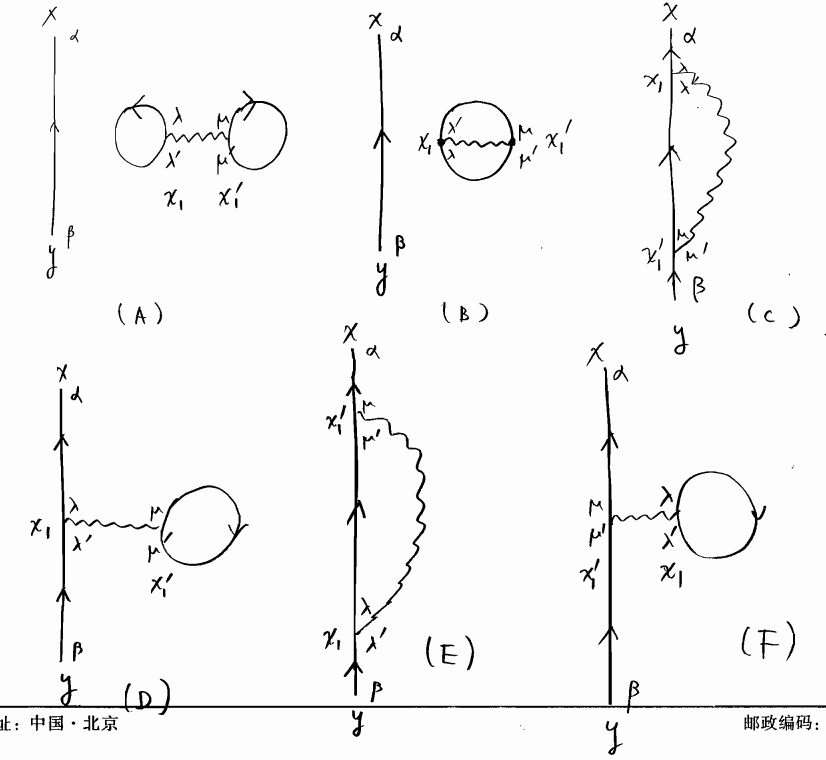
\includegraphics[width = 12cm]{P245.png}
\end{center}
In this pictorial description, single-particle non-interacting green function $G^0$ is denoted by a straight line, with an arrow which runs from the second argument of $G^0$ to the first argument of $G^0$.

The interaction potential is denoted by a wavy line, to distinguish with straight fermi line%???

	There are several features in these first order expressions.

1.First of all, these three terms contain a green's function whose two arguments are at the same time.
\begin{align}
\mathrm{i}G^0_{\alpha\beta}(x,x)\stackrel{?}{=}\langle\Phi_0|\mathrm{T}[\hat \psi_{\alpha}({\bf x},t)\hat \psi_{\beta}^{\dagger}({\bf x},t)]|\Phi_0\rangle \nonumber
\end{align}
By definition, such a green function (has an ambiguity, in a sense that it) could be either this or this.
\begin{align}
\stackrel{?}{=}
\begin{cases}
\langle\Phi_0|\hat \psi_{\alpha}({\bf x},t)\hat \psi_{\beta}^{\dagger}({\bf x},t)|\Phi_0\rangle  \cr \langle\Phi_0|\hat \psi_{\alpha}({\bf x},t)\hat \psi_{\beta}^{\dagger}({\bf x},t)|\Phi_0\rangle
\end{cases}
\nonumber
\end{align}
This ambiguity comes from the interaction Hamiltonian, where two creation operators and two annihilation operator have the same time argument
$$(r.h.s)=\langle\Phi_0|\mathrm{T}[\hat \psi_{\lambda}^{\dagger}(x_1)\hat \psi_{\mu}^{\dagger}(x_1')\hat \psi_{\mu'}(x_1')\hat \psi_{\lambda'}(x_1)\hat \psi_{\alpha}(x)\psi^{\dagger}_{\beta}(y)]|\Phi_0\rangle $$
To remove this ambiguity, we take the time argument of the two creation fields to be infinitesimally later than the time argument of the two annihilation fields.
$$(r.h.s)=\langle \Phi_0|\mathrm{T}[\hat \psi_{\lambda}^{\dagger}({\bf x}_1,t_1+0)\hat \psi_{\mu}^{\dagger}({\bf x}_1',t_1+0)\hat \psi_{\mu'}^{\dagger}({\bf x}_1',t_1)\hat \psi_{\lambda'}^{\dagger}({\bf x}_1,t_1)\hat \psi_{\alpha}(x)\hat \psi^{\dagger}_{\beta}(y)]|\Phi_0\rangle$$
This treatment is ok, because under the time-ordered product, this infinitesimally small factor can maintain the order of these four fields in the interaction Hamiltonian.

This small factor results in a small factor here so that, the green's function at equal times must be interpreted in this way.
\begin{align}
\mathrm{i}G_{\alpha\beta}^{0}(x,x)\equiv& \lim_{t'\rightarrow t+0} \langle \Phi_0 | \mathrm{T}[\hat\psi_{\alpha}({\bf x},t)\hat{\psi_{\beta}^{\dagger}}({\bf x},t')]|\Phi_0\rangle \nonumber \\
=&-\langle \Phi_0 |\hat{\psi_{\beta}^{\dagger}}({\bf x},t)\hat\psi_{\alpha}({\bf x},t)|\Phi_0\rangle \nonumber \\
=&-\delta_{\alpha\beta}n^0({\bf x}) \nonumber
\end{align}
where $n^0(x) $ is the particle density at x in the non-interacting ground state wave function.

For a uniform system, this can be replaced by a constant(N/V).

2. 2nd important features in this expression is that these two terms are  disconnected diagrams, in a sense that they contain subunits that are not connected to the rest of the diagrams.

eq.\eqref{2.5.2}shows that such disconnected diagrams typically have green's function and interaction whose arguments close within themselves.

As a result, these disconnected subunits can be factorized in the expression for $\tilde{G}$.

To see this, let us substitute eq.\eqref{2.5.2} into eq.\eqref{2.5.1} .
\begin{align}
\mathrm{i}\tilde{G_{\alpha\beta}}(x,y)=&\mathrm{i}\hat{G_{\alpha\beta}^0}(x,y)+(\frac{-\mathrm{i}}{\hbar})\sum_{\lambda\lambda'\mu\mu'}\frac{1}{2}\int\mathrm{d}^4x_1\mathrm{d}^4x_1' \nonumber \\
&\times \hat{U}_{\lambda\lambda'\mu\mu'}(x_1,x_1') \nonumber \\
&\times\{\mathrm{i}G_{\alpha\beta}^0(x,y)[\mathrm{i}G^0_{\mu'\mu}(x_1',x_1')\mathrm{i}G^0_{\lambda'\lambda}(x_1,x_1)-\mathrm{i}G^0_{\mu'\lambda}(x_1',x_1)\mathrm{i}G^0_{\lambda'\mu}(x_1,x_1')]\nonumber \\
&\ \ +(C)+(D)+(F)+(E)\} \nonumber
\end{align}
Since the arguments of this non-interacting green's function has nothing to do with these integral variables, we can rewrite this as
\begin{align}
=&\{\mathrm{i}G_{\alpha\beta}^0(x,y)+(\frac{-\mathrm{i}}{\hbar})\sum_{\lambda\lambda'\mu\mu'}\frac{1}{2}\int\mathrm{d}^4x_1\mathrm{d}^4x_1' \nonumber \\
&\ \ \hat{U}_{\lambda\lambda'\mu\mu'}(x_1,x_1')[(C)+(D)+(E)+(F)]+...\} \nonumber \\
&\times \{1+(\frac{-\mathrm{i}}{\hbar})\sum_{\lambda\lambda'\mu\mu'}\frac{1}{2}\int\mathrm{d}^4x_1\mathrm{d}^4x_1'\hat{U}_{\lambda\lambda'\mu\mu'}(x_1,x_1') \nonumber \\
&\ \ [\mathrm{i}G^0_{\mu'\mu}(x_1',x_1')\mathrm{i}G^0_{\lambda'\lambda}(x_1,x_1)-\mathrm{i}G^0_{\mu'\lambda}(x_1',x_1)\mathrm{i}G^0_{\lambda'\mu}(x_1,x_1')]+...\} \nonumber
\end{align}
where the product between this \& this gives the 0th order, while the product between this and these two give the 1st order disconnected diagrams, namely (A)\&(B) respectively.

On the other hand, the product between this 4 terms and this gives the 1st order connected diagrams, namely (C),(D),(E),(F).

One might also wonder about the product between these four \& these two.

Such a product reproduce exactly some of the 2nd-order disconnected diagrams obtained from the 2nd-order expansions.

To perform this factorization more systematically, let us consider the $\nu$-th order term of the numerator of eq.\eqref{2.4.4}:

\begin{align}
\mathrm{i}G_{\alpha\beta}^{(\nu)}(x,y)\equiv(\frac{-\mathrm{i}}{\hbar})^{\nu}\frac{1}{\nu!}\int_{-\infty}^{\infty}\mathrm{d}t_1...\int_{-\infty}^{\infty}\mathrm{d}t_{\nu}\langle\Phi_0|\mathrm{T}[\hat H_1(t_1)\hat H_1(t_2)...\hat H_1(t_{\nu})\hat \psi_{\alpha}(x)\hat \psi^{\dagger}_{\beta}(y)]|\Phi_0\rangle \nonumber
\end{align}
In general, $\nu$-numbers of interaction Hamiltonians can be divided into n-numbers of those interaction Hamiltonians which are connected to\ \ the fermion line running from y to x\ \ and m-numbers of those interaction Hamiltonians which are disconnected from the fermion line.
\begin{center}
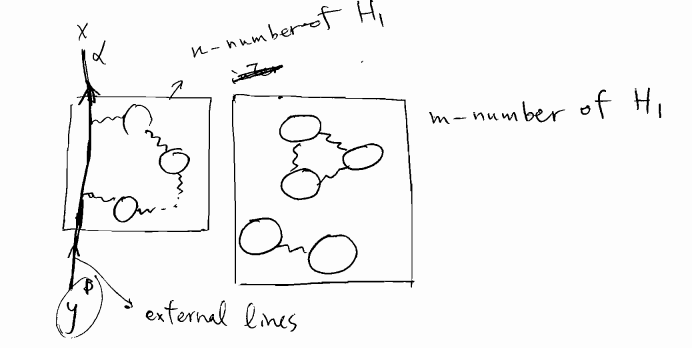
\includegraphics[width = 10cm]{P255.png}
\end{center}
The arguments appearing in the former group and those in the latter are nothing to do with each other, so that we can rewrite this into a product between two totally disconnected factors.

\begin{align}
\mathrm{i}\tilde{G}_{\alpha\beta}^{(\nu)}(x,y)=& \sum_{n=0}^{\nu}\sum_{m=0}^{\nu}(\frac{-\mathrm{i}}{\hbar})^{n+m}\frac{1}{\nu!}\frac{\nu!}{n!m!} \nonumber \\
&\int_{-\infty}^{\infty}\mathrm{d}t_1...\int_{-\infty}^{\infty}\mathrm{d}t_{m}\langle\Phi_0|\mathrm{T}[\hat H_1(t_1)...\hat H_1(t_{m})\hat \psi_{\alpha}(x)\hat \psi^{\dagger}_{\beta}(y)]|\Phi_0\rangle_{connected} \nonumber \\
&\int_{-\infty}^{\infty}\mathrm{d}t_{m+1}...\int_{-\infty}^{\infty}\mathrm{d}t_{m+n}\langle\Phi_0|\mathrm{T}[\hat H_1(t_{m+1})...\hat H_1(t_{m+n})\hat \psi_{\alpha}(x)\hat \psi^{\dagger}_{\beta}(y)]|\Phi_0\rangle \nonumber 
\end{align}
Here we put subscript 'connected', in order to emphasize that the contractions here must be taken in the 'connected' way like this diagram.

We also put this factor, because the numbers of ways of dividing $\nu$-number of interaction Hamiltonians in to n- number of the former group and m-number of the latter group is given by the factorial of $\nu$ divided by that of m times that of n.

When summed over the integer $\nu$ from zero to infinite, we obtain the numerator of eq.\eqref{2.4.4} as follows
\begin{align}
\mathrm{i}\tilde{G}_{\alpha\beta}^{(\nu)}(x,y)=& \sum_{m=0}^{\infty}(\frac{-\mathrm{i}}{\hbar})^{m}\frac{1}{m!}\int_{-\infty}^{\infty}\mathrm{d}t_1...\int_{-\infty}^{\infty}\mathrm{d}t_{m}\langle\Phi_0|\mathrm{T}[\hat H_1(t_1)...\hat H_1(t_{m})\hat \psi_{\alpha}(x)\hat \psi^{\dagger}_{\beta}(y)]|\Phi_0\rangle_{connected} \nonumber \\
&\times\sum_{m=0}^{\infty}(\frac{-\mathrm{i}}{\hbar})^{n}\frac{1}{n!}\int_{-\infty}^{\infty}\mathrm{d}t_1...\int_{-\infty}^{\infty}\mathrm{d}t_{n}\langle\Phi_0|\mathrm{T}[\hat H_1(t_1)...\hat H_1(t_{n})\hat \psi_{\alpha}(x)\hat \psi^{\dagger}_{\beta}(y)]|\Phi_0\rangle\nonumber 
\end{align}
Here the first factor is the sum of all connected Feynman diagrams.

On the other hand, the 2nd factor is identical to the denominator of eq.\eqref{2.4.4}
\begin{align}
\langle\Phi_0|\hat{S}|\Phi_0\rangle=&\langle\Phi_0|\hat{U}(+\infty,-\infty)|\Phi_0\rangle \nonumber \\
=&\langle\Phi_0|\sum_{\nu=0}^{\infty}(\frac{-\mathrm{i}}{\hbar})^{\nu}\frac{1}{\nu!}\int_{-\infty}^{\infty}\mathrm{d}t_1...\int_{-\infty}^{\infty}\mathrm{d}t_{\nu}\mathrm{T}[\hat H_1(t_1)...\hat H_1(t_{\nu})]|\Phi_0\rangle\nonumber 
\end{align}
So that the second factor are set off by the denominator, and eq.\eqref{2.4.4} is given by the sum of all possible connected Feynman diagrams.
\begin{align} \label{2.5.3}
\mathrm{i}G_{\alpha\beta}(x,y)=& \sum_{m=0}^{\infty}(\frac{-\mathrm{i}}{\hbar})^{m}\frac{1}{m!}\int_{-\infty}^{\infty}\mathrm{d}t_1...\int_{-\infty}^{\infty}\mathrm{d}t_{m}\langle\Phi_0|\mathrm{T}[\hat H_1(t_1)...\hat H_1(t_{m})\hat \psi_{\alpha}(x)\hat \psi^{\dagger}_{\beta}(y)]|\Phi_0\rangle
\end{align}
This formula for single-particle green's function is very useful, because it allows us to ignore all disconnected Feynman diagrams, which contain subunits not connected to the fermion line running from y to x.

3. The 3rd important remark is that, for any given connected diagram, there are many similar diagrams that differ in the permutation of the labels in the interaction Hamiltonian $\hat H_1$.

For example, these two diagrams 
\begin{center}
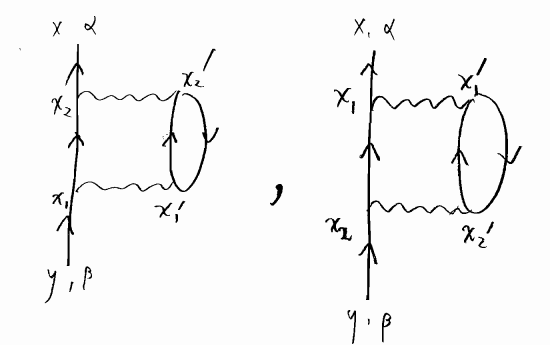
\includegraphics[width = 8cm]{P260.png}
\end{center}
differ from each other only in the permutation of the labels 1 \& 2 associated with the interaction Hamiltonian.

When these arguments are integrated oyut, these two give an identical contribution.

Another example is the 3rd order connected diagram shown here.
\begin{center}
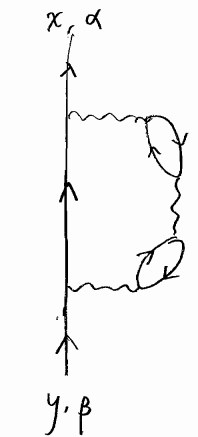
\includegraphics[width = 2cm]{P261.png}
\end{center}
Depending on how we assign three interaction Hamiltonians to these there wavy lines, we have 6 similar connected diagrams.

All of these six gives an identical contribution to the green's function.

For a m-th ordered connected diagram, we generally have the factorial of m number of similar diagrams, which differ in the permutations and all of which give an identical contribution.

This, 'the factorial of m' cancel the factor here.

Thus, for a given topologically distinct connected Feynman diagram, we count only once, while omitting this prefactor.

Here the 'topological distinct' means as follows

We regard that two diagrams are topologically distinct, when they cannot be transformed to each other, by any kind of deformation of wavy lines (interaction Hamiltonians).
\begin{center}
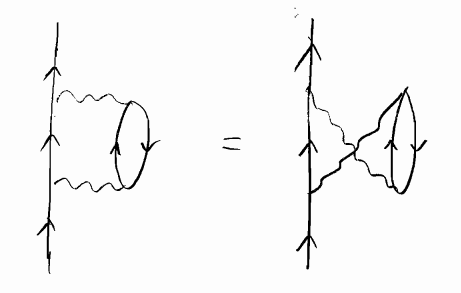
\includegraphics[width = 6cm]{P263.png}
\end{center}
4. Note also that, in the first order examples shown in eq.\eqref{2.5.2}, the terms (C)\&(E) are equal to each other.

They differ only in that x\&x' are interchanged, while the potential is symmetric under this interchange
$$U_{\lambda\lambda',\mu\mu'}(x,x')=U_{\mu\mu',\lambda\lambda'}(x',x)$$
Accordingly, it is sufficient to retain just one of these two, while omitting prefactor $\frac{1}{2}$ which appears in $\hat V$ in eq.\eqref{2.3.3}


The same is true for (D)\&(F).

We therefore obtain the following rules for calculating the n-th order contribution to the single particle green's function.

(a) Draw all topologically distinct connected Feynman diagrams, with n-interaction lines U and (2n+1) directed green's function $G^0$

(b) Label each vertex with a for dimensional space-time coordinate.

(c) Each solid line represents a green's function $G_{\alpha\beta}^0(x,y)$ running for y to x.

(d) Each wavy lines represents an interaction.
\begin{center}
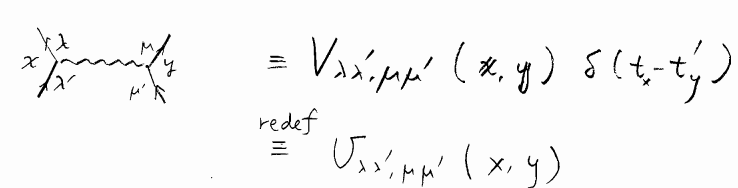
\includegraphics[width = 10cm]{P266.png}
\end{center}
(e) integrate all the internal variables over space and time.

(f) take the sum over all the spin indices associated with internal lines.

Since the n-th order term in eq.\eqref{2.5.3} has an explicit numerical factor $(\frac{-\mathrm{i}}{\hbar})^n$

Each contraction of two field operators gives $\mathrm{i}G^0$, so that (2n+1) contractions of the field operators gives $(\mathrm{i})^{2n+1}$

(g) for each n-th order term for G, assign $(-\mathrm{i})(\mathrm{i})^{2n+1}(\frac{-\mathrm{i}}{\hbar})^n=(\frac{-\mathrm{i}}{\hbar})^n$

in addition to this, each Feynman diagram must be accompanied by  either (+) or (-) sign, which comes from the rearrange process of the field operators.

Namely, when we obtained eq.\eqref{2.5.2}, we have rearranged the order of operators, in such a way that two field operators that are contracted are brought together.

Depending on whether this rearrange process is accompanied by even numbers of permutations of field operators or odd numbers of the permutations, each Feynman diagram is accompanied by (+) or (-) sign respectively.

Generally, a Feynman diagram with F-numbers of loops composed by fermion lines is accompanied by $(-1)^F$
\begin{center}
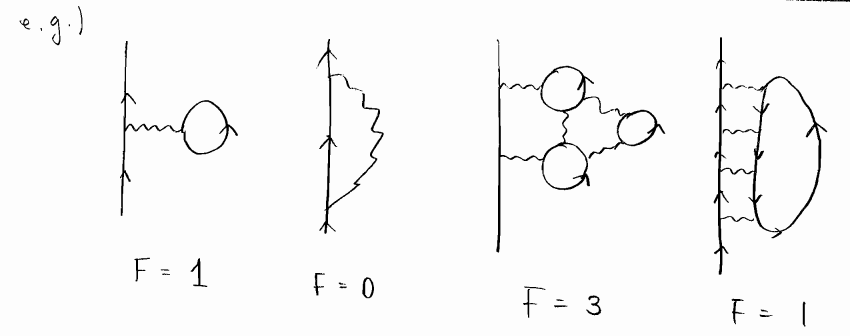
\includegraphics[width = 12cm]{P270-1.png}
\end{center}
This can be in the following way.

Generally speaking, any loop in a Feynman diagram is given like this.
\begin{center}
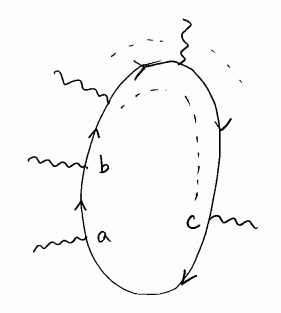
\includegraphics[width = 3cm]{P270-2.png}
\end{center}

On the one hand, according to eq.(A), the starting order of the field operators is given like this.

$$\mathrm{T}[\hat H_1(t_1)...\hat H_1(t_a)...\hat H_1(t_b)...\hat H_1(t_c)...\hat H_1(t_m)\hat \psi_{\alpha}(x)\hat \psi_{\beta}^{\dagger}(y)]$$
\begin{center}
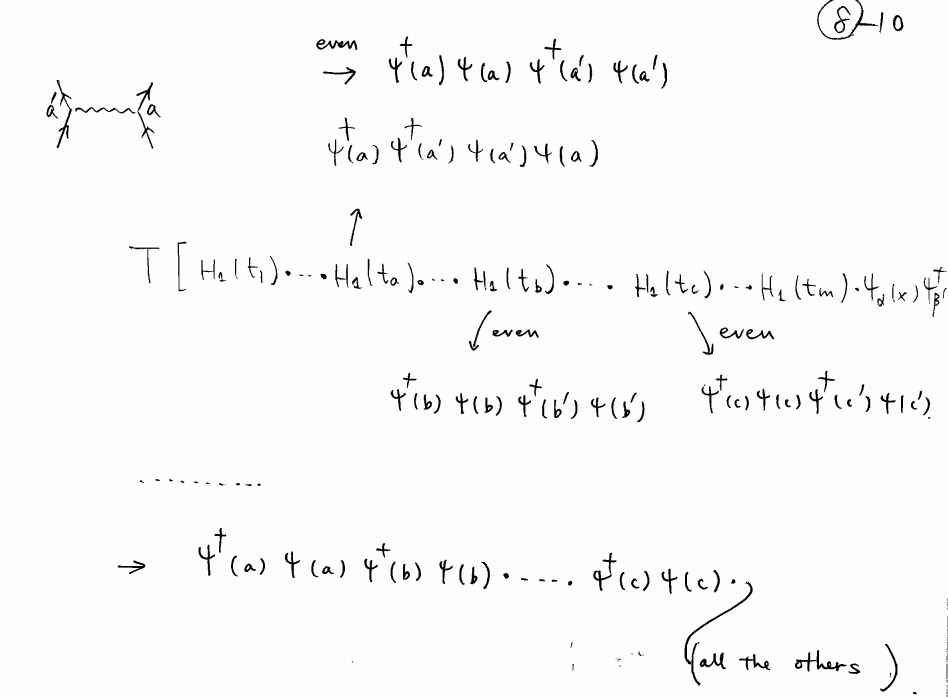
\includegraphics[width = 14cm]{P271.png}
\end{center}
Where these three interaction Hamiltonians correspond to these three wavy lines respectively.

Each interaction Hamiltonian can be given like this, and corresponding Feynman diagram is depicted like this.

Under the time-ordered product, we can rearrange this like this with even number of permutation.

Similarly we can do this for other interaction Hamiltonians.
\begin{center}
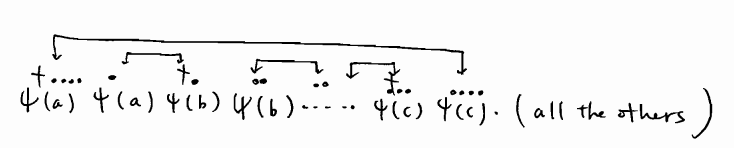
\includegraphics[width = 12cm]{P273.png}
\end{center}

Now that this part corresponds to this part and this part corresponds to this part, so that we bring them together like this.

This rearranging process is accompanied by even number of permutations, because these pairs of two fields always move together.

Then, according to this diagram, we take contractions like this.
\begin{center}
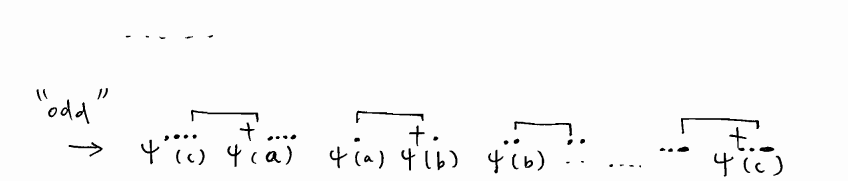
\includegraphics[width = 11cm]{P275.png}
\end{center}

Then, most of the two fields that are contracted are already brought together, except for these two fields.

But, when we bring together these two, we always need odd numbers of permutations.

This concludes that, for each loop of fermion fields, we always have one minus sign.
\begin{center}
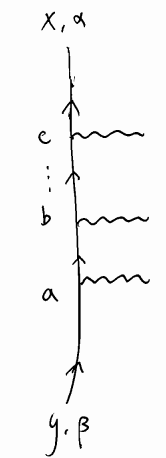
\includegraphics[width = 2cm]{P277.png}
\end{center}

We can do the same procedure for the other loops which you can find within all the others.

By construction, the remaining fermion fields comprise a single fermion lines which runs from y to x, where and x are associated with the external fermion fields which can be depicted like this
\begin{align}
&\mathrm{T}[\hat H_1(t_1)...\hat H_1(t_a)...\hat H_1(t_b)...\hat H_1(t_c)...\hat H_1(t_m)\hat \psi_{\alpha}(x)\hat \psi_{\beta}^{\dagger}(y)]\nonumber \\
=&(-1)^F\mathrm{T}[(loop1)(loop2)...(loopF)\hat \psi^{\dagger\cdot\cdot\cdot\cdot\cdot}(a)\hat \psi^{\cdot}(a)\hat \psi^{\cdot\cdot\cdot\cdot}(b)...\hat \psi^{\dagger\cdot\cdot\cdot}(c)\hat \psi^{\cdot\cdot\cdot\cdot}(c)\hat \psi_{\alpha}^{\cdot\cdot\cdot\cdot}(x)\hat \psi_{\beta}^{\dagger\cdot\cdot\cdot\cdot}(y)]\nonumber
\end{align}
With even number of permutations, all the remaining fermion fields can be rearranged in this way.

According to this picture, we take the contraction like this, where most of the two fields that are contracted are already brought together.

except for these two field.

When we bring together these two, we need even number of permutations, because here we have even numbers of field operators.
\begin{align}
=&(-1)^F\mathrm{T}[(loop1)(loop2)...(loopF)(the\ single\ fermion\ line)]\nonumber
\end{align}
This gives us this expression for this.

(h) To summarize, a Feynman diagram with F-numbers of fermion loops is always accompanied by $(-1)^F$

This is the 2nd last rule for the Feynman diagram calculations.

The final rule is for a non-interacting single particle green's function with equal time variables.

As I have already explained, the green's function with equal time variables should be interpreted as this way

(i) $G_{\alpha\beta}^0(x,t;x',t')\rightarrow G_{\alpha\beta}^0(x,t;x',t+0)$

\begin{center}
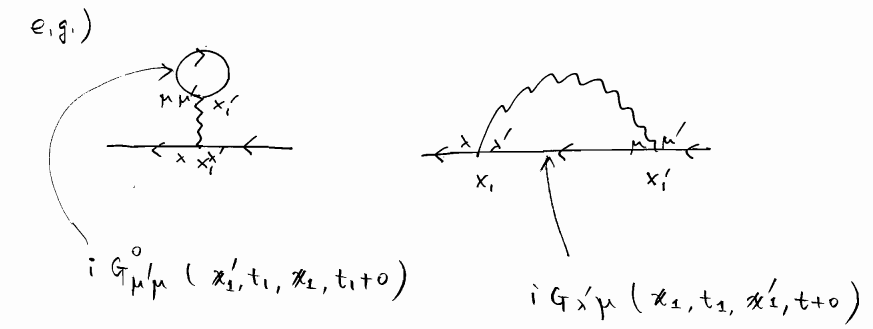
\includegraphics[width = 13cm]{P283.png}
\end{center}


This is all about the rules for the Feynman diagram calculations.

Based on this Feynman's rules, let us again calculate the 1st-order contribution to the single-particle green's function.

$$G_{\alpha\beta}^{(1)}(x,y)=?$$
Only the topologically distinct connected Feynman diagrams are just these two.
\begin{center}
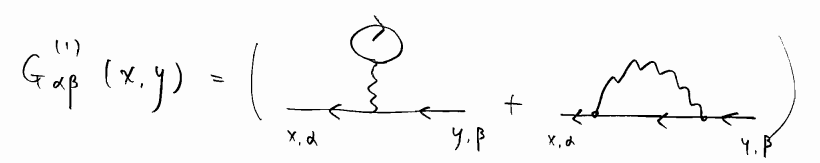
\includegraphics[width = 12cm]{P284-1.png}
\end{center}
By labelling these vertex four dimensional coordinate,
\begin{center}
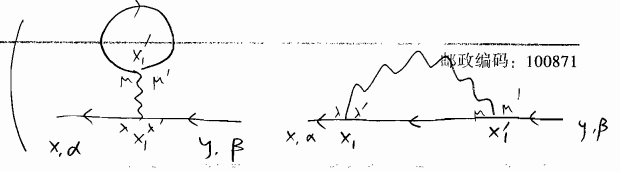
\includegraphics[width = 8cm]{P284-2.png}
\end{center}

According to the rule, we assign each fermion line with $G^0$ and a wavy line with V. so that we obtain

\begin{align}\label{2.5.4}
G_{\alpha\beta}^{(1)}(x,y)=&(\frac{\mathrm{i}}{\hbar})\int \mathrm{d}^4x_1\int \mathrm{d}^4x_1' \nonumber \\
&\{-U_{\lambda\lambda'\mu\mu'}(x_1,x_1')G_{\alpha\lambda}^0(x,x_1)G_{\lambda'\beta}^0(x_1,y)G_{\mu'\mu}^0(x_1',x_1') \nonumber \\
&\ +U_{\lambda\lambda'\mu\mu'}(x_1,x_1')G_{\alpha\lambda}^0(x,x_1)G_{\lambda'\mu}^0(x_1,x_1')G_{\mu'\beta}^0(x_1',y)\} 
\end{align}

The second-order contribution can be enumerated like this.
\begin{center}
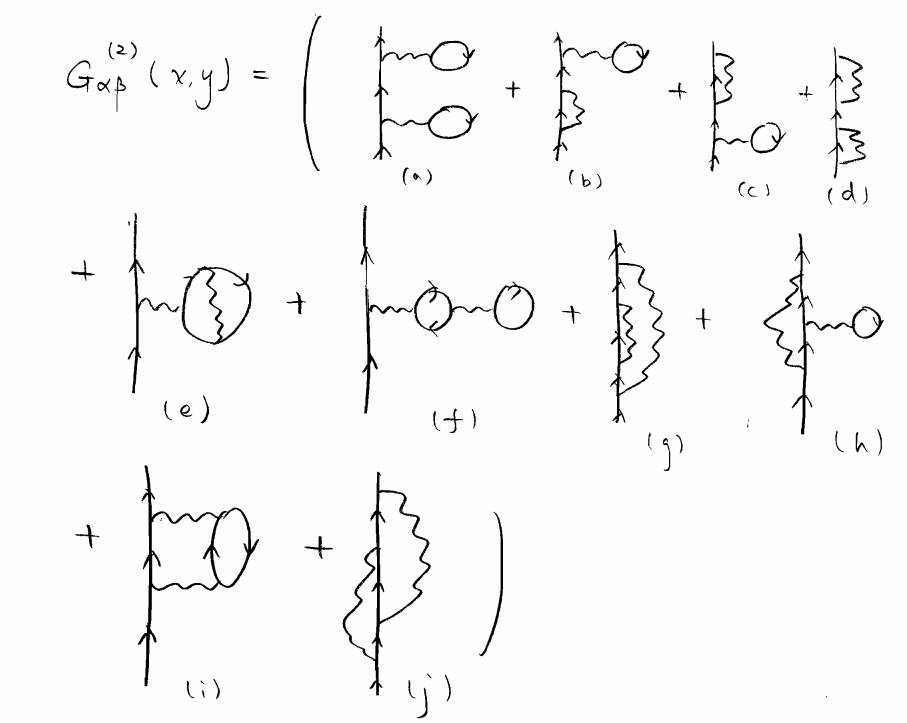
\includegraphics[width = 13cm]{P286.png}
\end{center}
which exhaust all the 2nd-order topologically distinct connected diagrams.

Writing the corresponding equations for all of these diagrams is a bit cumbersome, so that I only write down one of them.

For example, consider the lase one
\begin{center}
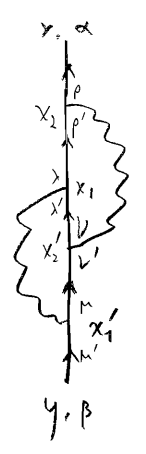
\includegraphics[width = 2cm]{P287.png}
\end{center}
\begin{align}
G^{(2)}_{\alpha\beta}(x,y)=...&+(\frac{\mathrm{i}}{\hbar})^2\int \mathrm{d}^4x_1\int \mathrm{d}^4x_1'\int \mathrm{d}^4x_2\int \mathrm{d}^4x_2'U_{pp'\nu\nu'}(x_2,x_2')U_{\lambda\lambda'\mu\mu'}(x_1,x_1') \nonumber \\
&G_{\alpha\beta}^0(x,x_2)G_{p\lambda}^0(x_2,x_1)G_{\lambda'\nu}^0(x_1,x_2')G_{\nu'\mu}^0(x_2',x_1')G_{\mu'\beta}^0(x_1',y) \nonumber
\end{align}
Here, we don't have any (-) sign, because the diagram doesn't contain any fermion's loop.

Observing this expression, one can see that actual evaluations of each terms are highly involved, in a sense that, even 2nd order term requires integral over four internal variables.

To reduce these complications, let us now restrict the following discussions to a spatially uniform (and spin-isotropic) system.

In such a system, the green's function take the form like this 
$$G_{\alpha\beta}(x,y)=G_{\alpha\beta}(x-y)$$

This form allows us to take a fourier transformation
\begin{align}\label{2.5.5}
G_{\alpha\beta}(x,y)\equiv\frac{1}{(2\pi)^4}\int \mathrm{d}^4ke^{\mathrm{i}k(x-y)}G_{\alpha\beta}(k) \nonumber \\
G^0_{\alpha\beta}(x,y)\equiv\frac{1}{(2\pi)^4}\int \mathrm{d}^4ke^{\mathrm{i}k(x-y)}G^0_{\alpha\beta}(k)
\end{align}
with
$$\mathrm{d}^4k=\mathrm{d}^3\bf{k}\mathrm{f}\omega$$

$$k\cdot x=\bf{k}\cdot\bf{x}-\omega t$$
In a spatially homogeneous system, the interaction potential depends only on the coordinate difference.
\begin{align}\label{2.5.6}
U(x,x')\equiv& V(\bf{x},\bf{x}')\delta(t-t') \nonumber \\
=& V(\bf{x}-\bf{x}')\delta(t-t')
\end{align}
Such a potential can be also fourier-transformed
$$U_{\alpha\alpha\beta\beta'}(x,x')\equiv \frac{1}{(2\pi)^4}\int \mathrm{d}^4ke^{\mathrm{i}k(x-x')}U_{\alpha\alpha\beta\beta'}(k)$$
where
\begin{align}\label{2.5.7}
U_{\alpha\alpha\beta\beta'}(k)=\int \mathrm{d}^3x e^{-\mathrm{i}\bf{k}\cdot\bf{x}}V_{\alpha\alpha\beta\beta'}({\bf x}) \ \ (E)
\end{align}
(with the use of $\delta(t)=\frac{1}{2\pi}\int \mathrm{d}\omega e^{-\mathrm{i}\omega t}$)

Using this transformation, eq.\eqref{2.5.4} can be substantially simplified:
\begin{center}
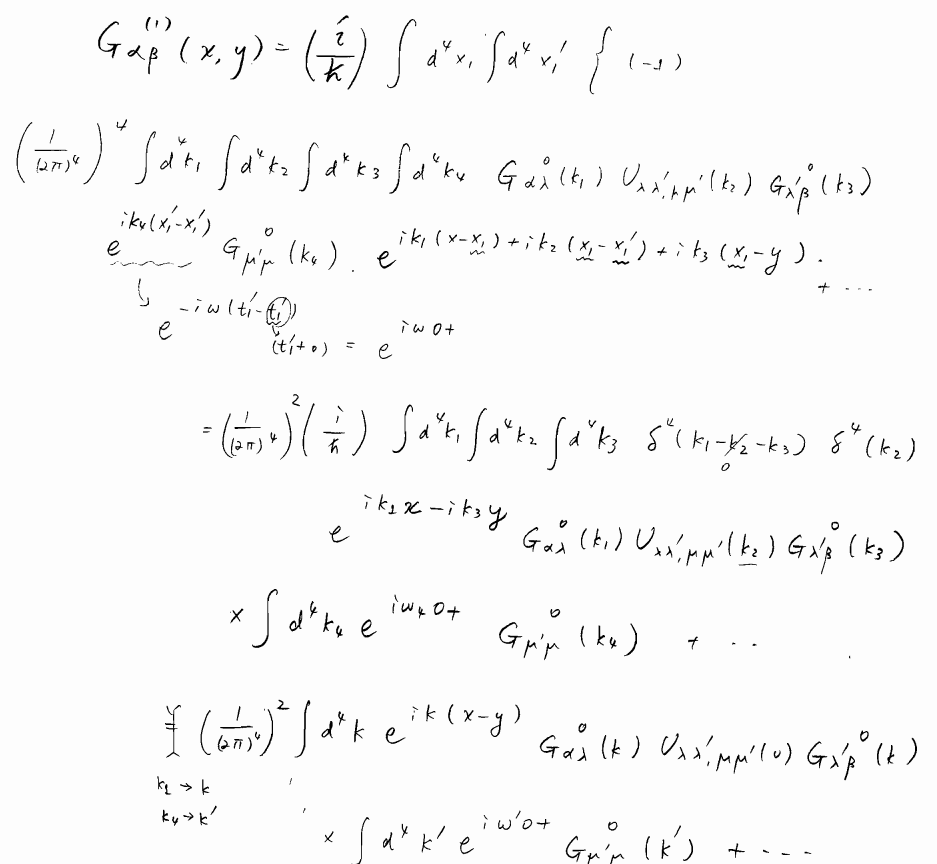
\includegraphics[width = 15cm]{P291.png}
\end{center}\begin{center}
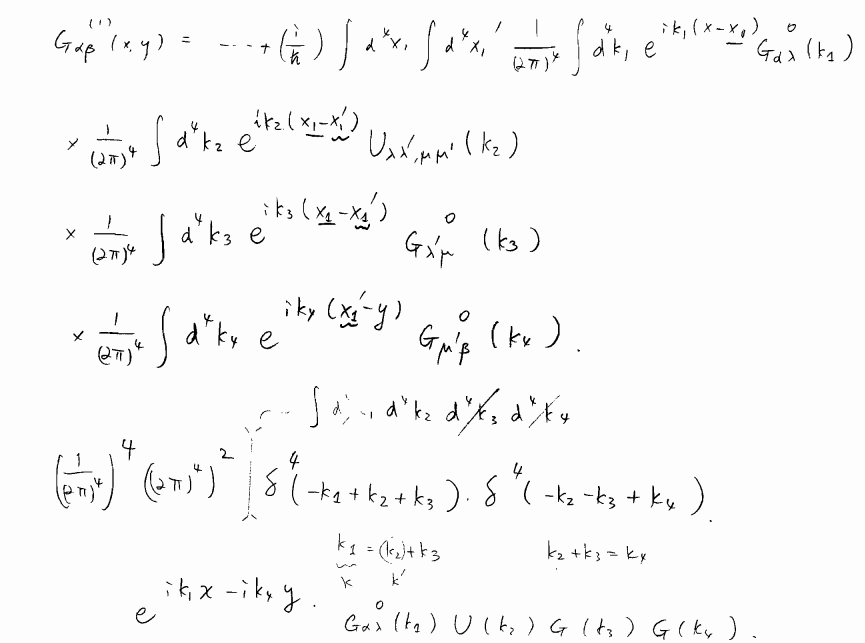
\includegraphics[width = 15cm]{P292.png}
\end{center}
\begin{align}
G_{\alpha\beta}^{(1)}(x,y)=&-\frac{\mathrm{i}}{\hbar}(\frac{1}{(2\pi)^4})^2\int \mathrm{d}^4ke^{\mathrm{i}k(x-y)}G_{\alpha\lambda}^0(k)U_{\lambda\lambda'\mu\mu'}(0)G_{\lambda'\beta}^0(k)\int \mathrm{d}^4k'e^{\mathrm{i}\omega'0+}G_{\mu'\mu}^0(k')\nonumber \\
&+\frac{\mathrm{i}}{\hbar}(\frac{1}{(2\pi)^4})^2\int \mathrm{d}^4ke^{\mathrm{i}k(x-y)}\int \mathrm{d}^4k'G_{\alpha\lambda}^0(k)U_{\lambda\lambda'\mu\mu'}(k')G_{\lambda'\mu}^0(k-k')G_{\mu'\beta}^0(k)\nonumber \\
\equiv & (\frac{1}{(2\pi)^4})^2\int \mathrm{d}^4ke^{\mathrm{i}k(x-y)}G_{\alpha\beta}^{(1)}(k) \nonumber
\end{align}
where $G_{\alpha\beta}^{(1)}(k)$ contains only momentum integral.
\begin{align}\label{2.5.8}
G_{\alpha\beta}^{(1)}(k)\equiv &-\frac{\mathrm{i}}{\hbar}(\frac{1}{(2\pi)^4})^2G_{\alpha\lambda}^0(k)U_{\lambda\lambda'\mu\mu'}(0)G_{\lambda'\beta}^0(k)\int \mathrm{d}^4k'e^{\mathrm{i}\omega'0+}G_{\mu'\mu}^0(k') \nonumber \\
&+\frac{\mathrm{i}}{\hbar}(\frac{1}{(2\pi)^4})^2G_{\alpha\lambda}^0(k)G_{\mu'\beta}^0(k)\int \mathrm{d}^4k'U_{\lambda\lambda'\mu\mu'}(k')G_{\lambda'\mu}^0(k-k')\ \ (F)
\end{align}
This momentum space representation can be generalized into the higher-order Feynman diagram.

Any Feynman diagram comprise a vertex show like this, in which one in-coming fermion line and one out-going fermion line and interaction lines meet with on another
\begin{center}
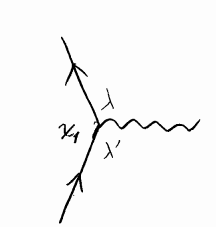
\includegraphics[width = 3cm]{P294.png}
\end{center}
Under the fourier transformation defined in eq.\eqref{2.5.5}, the in-coming fermion line provides $e^{\mathrm{i}qx_1}$, and the out-going fermion line provides $e^{-\mathrm{i}q'x_1}$
\begin{center}
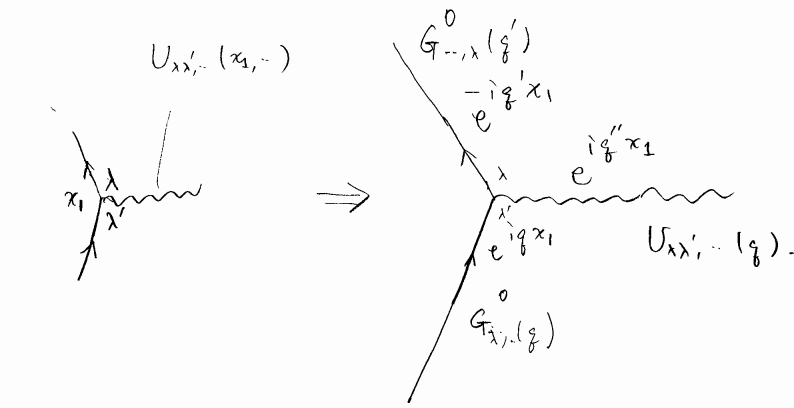
\includegraphics[width = 12cm]{P295.png}
\end{center}

where q and q' are the four-dimensional momenta associated with these two lines.

Namely, we assign this line with $G_{\lambda',...}^0(q)$ and assign this line with $G_{...,\lambda}^0(q')$.

When this interaction potential is given by $U_{\lambda\lambda',...}(x_1,...)$, where we assign the wavy line with $U_{\lambda\lambda',...}(q'')$.


For simplicity, we rewrite this picture like this.
\begin{center}
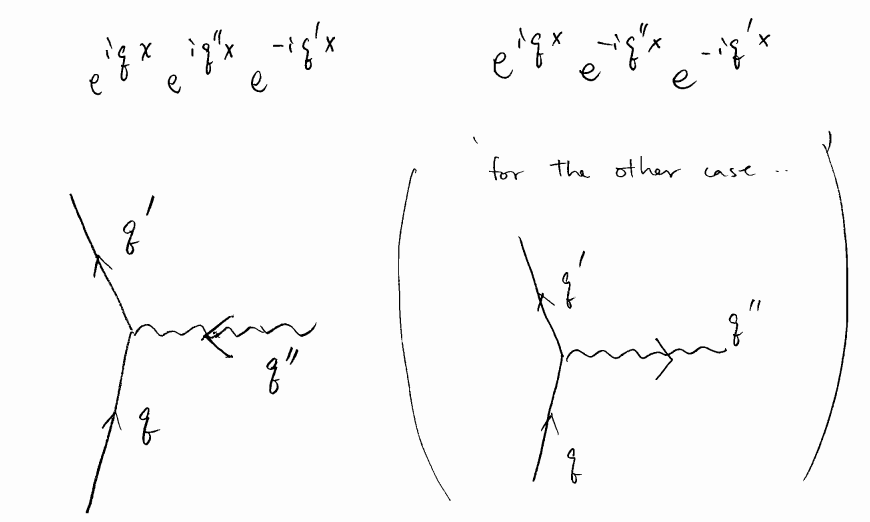
\includegraphics[width = 14cm]{P297.png}
\end{center}
In order to indicate this plus sign, we put another arrow here for the interaction line.

Namely, for this figure, we suppose that these three lines provide $e^{\mathrm{i}qx},e^{\mathrm{i}q''x},e^{-\mathrm{i}q'x}$ respectively.

while for the other case, we suppose that they provide $e^{\mathrm{i}qx},e^{-\mathrm{i}q''x},e^{-\mathrm{i}q'x}$ respectively.

Now that x here is the internal variable, we are supposed to take the integral over this.

Now that, for any given Feynman diagram which have this as its submit, there is no x-dependence other than these three phase factors.

Therefore, the integration over x gives a momentum conservation among these three.

\begin{align}
\int \mathrm{d}^4xe^{\mathrm{i}(q-q'+q'')x}=(2\pi)^4\delta^4(q-q'+q'') \nonumber
\end{align}

Namely, the sum of the two in-coming momenta must be equal to the out-going momentum.


Since every integral vertex provides the momentum conservation law, the in-coming momentum and out-going momentum conservation law, the in-coming momentum and out-going momentum for the external fermion fields are equal to each  other.
\begin{center}
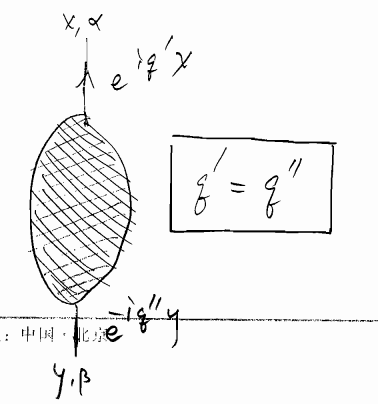
\includegraphics[width = 4cm]{P300.png}
\end{center}
You can check this equality for any Feynman diagram.

As an illustration, consider this 
\begin{center}
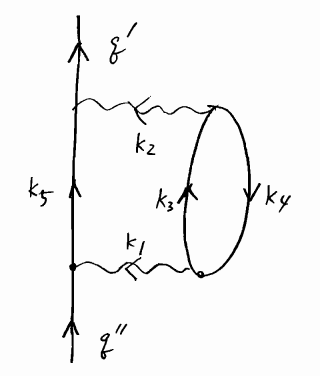
\includegraphics[width = 4cm]{P301.png}
\end{center}
you can assign arrows for wavy lines in an arbitrary way, so that I put this way.

Then we have these conservations for each internal vertex
$$k_5=k_1+q''$$$$k_3+k_1=k_4$$$$k_2+k_4=k_3$$$$q'=k_2+k_5$$$$q'=k_2+k_5=(k_3-k_4)+k_1+q''=k_4-k_4+q''=q''$$

From which  we safely obtain this equality.

To sumarize, the Feynman rule in the momentum space representation can be summarized as follows.

For the n-th order contribution to $$G_{\alpha\beta}({\bf k},\omega)\equiv G_{\alpha\beta}(k)$$

1. Draw all topologically distinct connected diagrams with n-interaction lines and (2n+1) fermion lines.

2. Assign momentum to fermion lines and interaction lines with arrows.

3. Correspondingly, we assign each fermion line with the non-interacting green's fn in the momentum space.(eq.\eqref{2.3.6})
$$G_{\alpha\beta}^0({\bf k},\omega)=\delta_{\alpha\beta}[\frac{\theta(|k|-k_F)}{\omega-\omega_k+\mathrm{i}\eta}+\frac{\theta(k_F-|k|)}{\omega-\omega_k-\mathrm{i}\eta}]$$

while we assign each wavy line with the interaction potential in the momentum space representation.
$$U_{\lambda\lambda',\mu\mu'}(q)\equiv V_{\lambda\lambda',\mu\mu'}({\bf q})$$

4. Impose momentum conservations at every internal vertex.

$(2n+1)+n-2n=n+1$

This conservation gives (n+1) independent momentum, where one of them should be reserved for the external line.

Thus we have n independent internal momenta, over which we need to take the integration.

5. Take a summation over internal spin indices.

As an overall factor, we originally have $(\frac{\mathrm{i}}{\hbar})^n(-1)^F$ in the Feynman rule in the real space representation.

During this fourier transformation process, we obtain
$$(\frac{1}{(2\pi)^4})^{2n+1}(\frac{1}{(2\pi)^4})^n((2\pi)^4)^{2n}=(\frac{1}{(2\pi)^4})^{n+1}$$

One of them should be again reserved for the external line, so that

6. For the n-th order Feynman diagram for $G_{\alpha\beta}(k)$, we need to apply $(\frac{\mathrm{i}}{\hbar})^n\frac{1}{(2\pi)^{4n}}(-1)^F$ as an overall factor

The final remark  is about a fermion line that form a closed loop like this or about a fermion line whose two end points are linked by the same interaction link (like this)
\begin{center}
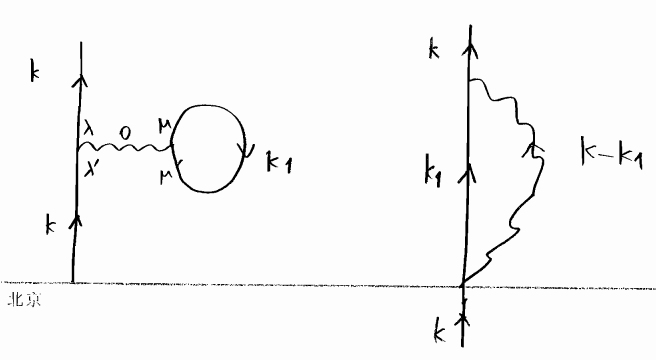
\includegraphics[width = 9cm]{P306.png}
\end{center}
These fermion lines are originally green's function with equal time variables, so that we assigned these green's function to them in this way.

7. When Fourie-transformed, this infinitesimally small factor is transformed with this additional factor, where $\eta$ is positive small quantity:
$$e^{\mathrm{i}\omega\eta}G_{\alpha\beta}({\bf k},\omega) \ \ (\eta\rightarrow0+)$$

With this Feynman rule, one can obtain eq.\eqref{2.5.8}

\begin{align}
G_{\alpha\beta}^{(1)}(k)=&-\frac{\mathrm{i}}{\hbar}\frac{1}{(2\pi)^4} G_{\alpha\lambda}^{(0)}(k)U_{\lambda\lambda'\mu\mu'}(0)G_{\lambda'\beta}^{(0)}(k)\int \mathrm{d}^4k'e^{\mathrm{i}\omega'0+}G_{\mu'\mu}^0(k') \nonumber \\
&+\frac{\mathrm{i}}{\hbar}\frac{1}{(2\pi)^4} G_{\alpha\lambda}^{(0)}(k)G_{\mu'\beta}^{(0)}(k)\int \mathrm{d}^4k'e^{\mathrm{i}\omega'0+}U_{\lambda\lambda'\mu\mu'}(k-k')G_{\lambda'\mu}^0(k') \nonumber
\end{align}

To make further progress, we decompose interaction potential U into spin independent part and spin dependent part 

\begin{align}
U_{\lambda\lambda'\mu\mu'}(q)\equiv& V_{\lambda\lambda'\mu\mu'}(q) \nonumber \\
=& V_0(q) \delta_{\lambda\lambda'}\delta_{\mu\mu'}+V_1(q)\sum_{\nu=1}^{3}[\sigma_{\nu}]_{\lambda\lambda'}[\sigma_{\nu}]_{\mu\mu'} \nonumber
\end{align}

where $\sigma_{1,2,3}$ are Pauli matrices.

Taking $G_{\alpha\beta}^0(k)=\delta_{\alpha\beta}G^0(k)$, we can rewrite eq.\eqref{2.5.8} as follows  
\begin{align}
G_{\alpha\beta}^{(1)}(k)=&-\frac{\mathrm{i}}{\hbar}\frac{1}{(2\pi)^4}\delta_{\alpha\lambda}G^{0}(k)
\nonumber \\
&\{V_0(0) \delta_{\lambda\lambda'}\delta_{\mu\mu'}+V_1(0)\sum_{\nu=1}^{3}[\sigma_{\nu}]_{\lambda\lambda'}[\sigma_{\nu}]_{\mu\mu'}\}\delta_{\lambda'\beta}G^0(k)\int \mathrm{d}^4k'e^{\mathrm{i}\omega'0+}\delta_{\mu\mu'}G^0(k')\nonumber \\
&+\frac{\mathrm{i}}{\hbar}\frac{1}{(2\pi)^4}\delta_{\alpha\lambda}G^0(k)\delta_{\mu'\beta}G^0(k)\int \mathrm{d}^4k'e^{\mathrm{i}\omega'0+}\nonumber\\
&\{V_0(k-k') \delta_{\lambda\lambda'}\delta_{\mu\mu'}+V_1(k-k')\sum_{\nu=1}^{3}[\sigma_{\nu}]_{\lambda\lambda'}[\sigma_{\nu}]_{\mu\mu'}\}\delta_{\lambda'\mu}G^0(k') \nonumber \\
with\ \mathrm{Tr}&[\sigma_{\nu}]=0\ \ for \ \nu=1,2,3 \nonumber \\
=&-\frac{\mathrm{i}}{\hbar}\frac{1}{(2\pi)^4}2\delta_{\alpha\beta}G^{0}(k)V_0(0)G^0(k)\int \mathrm{d}^4k'e^{\mathrm{i}\omega'0+}G^0(k')\nonumber \\
&+\frac{\mathrm{i}}{\hbar}\frac{1}{(2\pi)^4}\delta_{\alpha\beta}G^{0}(k)G^0(k)\int \mathrm{d}^4k'V_0(k-k')e^{\mathrm{i}\omega'0+}G^0(k')\nonumber \\
&+\frac{\mathrm{i}}{\hbar}\frac{1}{(2\pi)^4}3\delta_{\alpha\beta}G^{0}(k)G^0(k)\int \mathrm{d}^4k'V_1(k-k')e^{\mathrm{i}\omega'0+}G^0(k')\nonumber \\
\equiv& G^{0}(k)\Sigma^{(1)}(k)G^0(k)\delta_{\alpha\beta} \nonumber \\
\hbar \Sigma^{(1)}(k)=& \mathrm{i}\frac{1}{(2\pi)^4}3\int \mathrm{d}^4k'[-2V_0(0)+V_0(k-k')3V_1(k-k')]e^{\mathrm{i}\omega'0+}G^0(k') \nonumber
\end{align}
Thanks to this factor, we can integrate over frequency

\begin{align}
\int_{-\infty}^{\infty}\frac{\mathrm{d}\omega'}{2\pi}e^{\mathrm{i}\omega'0+}G^0({\bf k}',\omega')=\int_{-\infty}^{\infty}\frac{\mathrm{d}\omega'}{2\pi}e^{\mathrm{i}\omega'0+}[\frac{\theta(|k|-k_F)}{\omega-\omega_k+\mathrm{i}\eta}+\frac{\theta(k_F-|k|)}{\omega-\omega_k-\mathrm{i}\eta}]=\mathrm{i}\theta(k_F-|k'|) \nonumber
\end{align}
\begin{center}
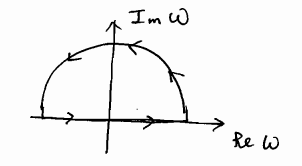
\includegraphics[width = 4cm]{P312.png}
\end{center}
so that
\begin{align}\label{2.5.9}
\hbar \Sigma^{(1)}(k)=&-\int \frac{\mathrm{d}{\bf k}'}{(2\pi)^3}[-2V_0(0)+V_0(k-k')3V_1(k-k')]\theta(k_F-|{\bf k}'|) \nonumber \\
=& n V_0(0)-\int \frac{\mathrm{d}{\bf k}'}{(2\pi)^3}[V_0(k-k')3V_1(k-k')]\theta(k_F-|{\bf k}'|) \ \ (G) 
\end{align}

As we will see soon, these gives us a renormalization of single particle energy in the non-interacting limit.

To see this, let us introduce a general argument which classify various contributions in an arbitrary Feynman diagrams.

The classification leads to a so-called Dyson equation, which makes the diagramatic analysis to be very useful.

Feynman rules suggests that the exact green's function consists of the non-interacting green's function plus all the connected terms with a free ("non-interacting") green's function at each ends.

This structure is schematically shown like this:
\begin{center}
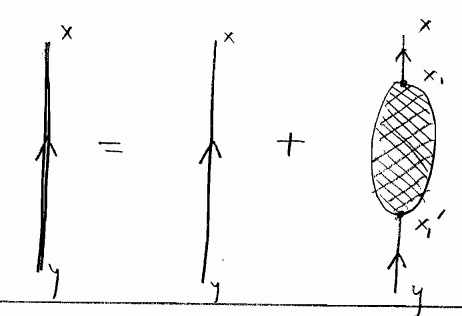
\includegraphics[width = 8cm]{P314.png}
\end{center}
The corresponding analytic expression is given by
$$G_{\alpha\beta}(x,y)=G_{\alpha\beta}^0(x,y)+\int \mathrm{d}^4x_1\int \mathrm{d}^4x_1'G_{\alpha\lambda}^0(x,x_1)\Sigma_{\lambda\mu}(x_1,x_1')G_{\mu\beta}^0(x_1,y)$$

$\Sigma$ corresponds to this part, which includes all the connected Feynman diagrams and is called as the self-energy

2nd-order examples for $\Sigma$ can be enumerated as follows
\begin{center}
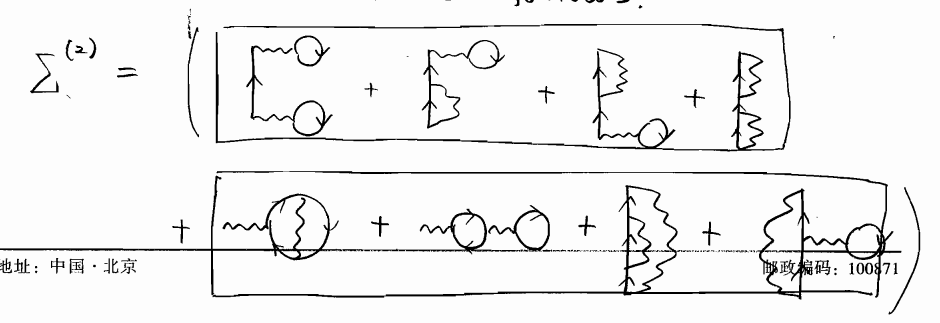
\includegraphics[width = 14cm]{P315.png}
\end{center}
Generally speaking, there are two types of self energy.

One is called as proper self-energy, which cannot be separated into two  pieces by cutting one fermion lines.

The other is called as inproper  self-energy, which can be separated into two pieces by cutting a fermion lines.

In this example, these are inproper ones, because, by cutting this line, they can be separated into two.

Especially, we will denote by $\Sigma^{\star}_{\alpha\beta}(x_1,x_1')$ the sum of all proper self-energy terms.

Then, thanks to the Feynman's rule described so far, the self-energy consists of a sum of all possible repetitions of the proper self-energy.
\begin{align}
\Sigma(x_1,x_1')=&\Sigma^{\star}(x_1,x_1?) \nonumber \\
&+\int \mathrm{d}^4x_2\mathrm{d}^4x_2'\Sigma^{\star}(x_1,x_2)G^0(x_2,x_2')\Sigma^{\star}(x_2',x_1?) \nonumber \\
&+\int \mathrm{d}^4x_2\mathrm{d}^4x_2'\int \mathrm{d}^4x_3\mathrm{d}^4x_3'\Sigma^{\star}(x_1,x_2)G^0(x_2,x_2')\Sigma^{\star}(x_2',x_1?)G^0(x_3,x_3')\Sigma^{\star}(x_3',x_1?)+... \nonumber
\end{align}
Which can be also described in terms of diagram as follows 
\begin{center}
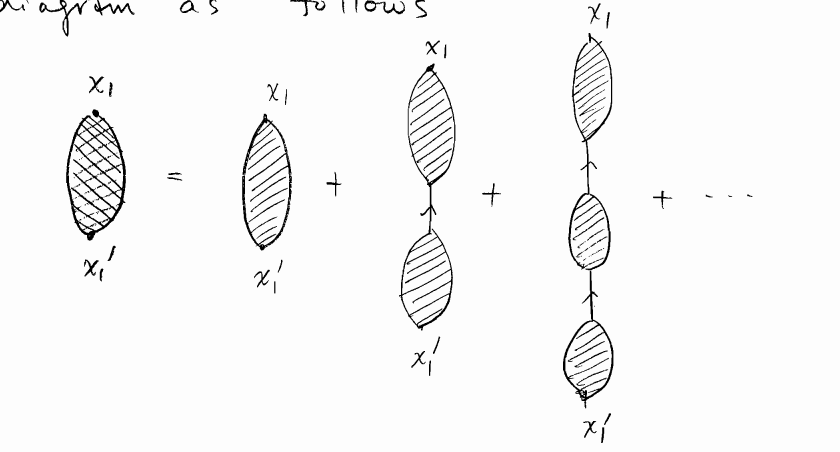
\includegraphics[width = 10cm]{P318.png}
\end{center}
Where this part denotes the proper self-energy, while this fermion line is for non-interacting green's function.

This description becomes possible, especially  because, any n-th order Feynman diagram is accompanied only by $(\frac{\mathrm{i}}{\hbar})^n(-1)^F$ where F denotes the number of fermion loop.

Namely, such a factor can be always decomposed like this
\begin{center}
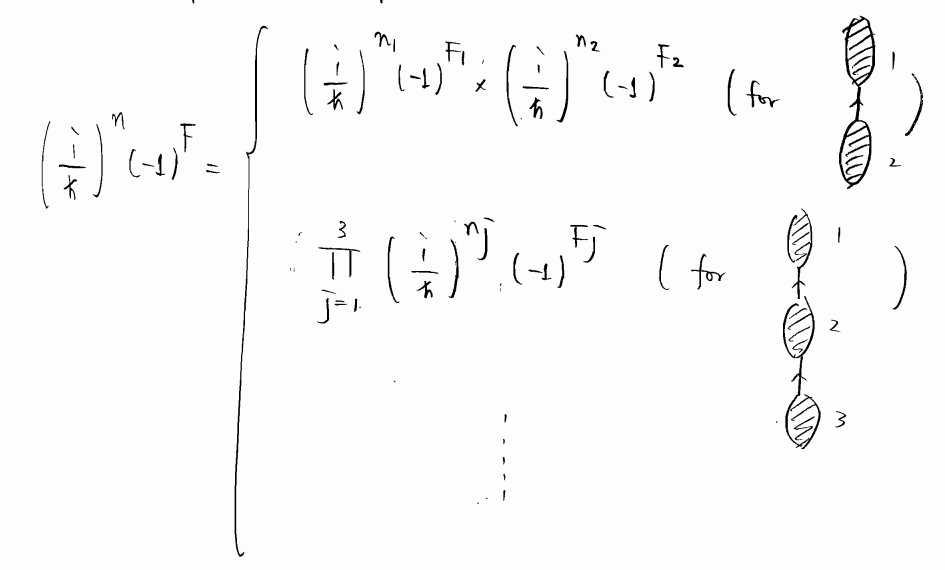
\includegraphics[width = 12cm]{P319.png}
\end{center}
Where $n_1\&n_2$ have denotes the number of wavy lines included in the 1st proper self-energy and 2nd proper self energy. so that $n_1+n_2=n$

Similarly $F_1\&F_2$ denotes the numbers of fermion loops included in these two proper self-energy respectively. so that $F_1+F_2=F$

Correspondingly, the single-particle green's function becomes like this
\begin{align}
G(x,y)=&G^0(x,y) \nonumber \\
&+\int \mathrm{d}^4x_1\mathrm{d}^4x_1'G^0(x,x_1)\Sigma^{\star}(x_1,x_1?)G^0(x_1',y) \nonumber \\
&+\int \mathrm{d}^4x_1\mathrm{d}^4x_1'\int \mathrm{d}^4x_2\mathrm{d}^4x_2'G^0(x,x_1)\Sigma^{\star}(x_1,x_1?)G^0(x_1',x_2)\Sigma^{\star}(x_2,x_2')G^0(x_2',y)+... \nonumber
\end{align}
or
\begin{center}
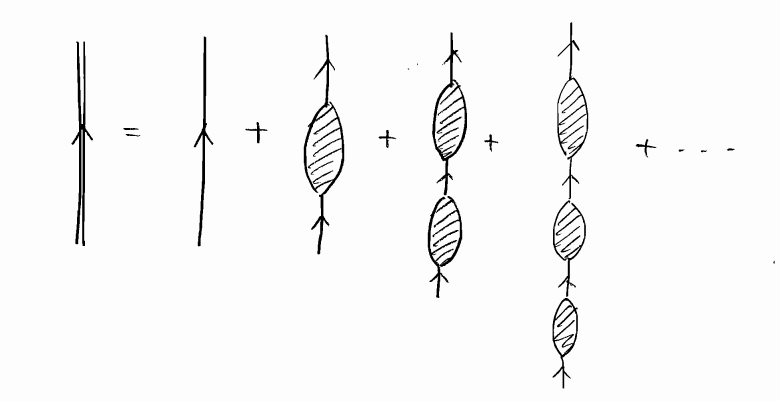
\includegraphics[width = 9cm]{P320.png}
\end{center}
As is clear from this repetitive structure, this can be rewritten also like this.
\begin{center}
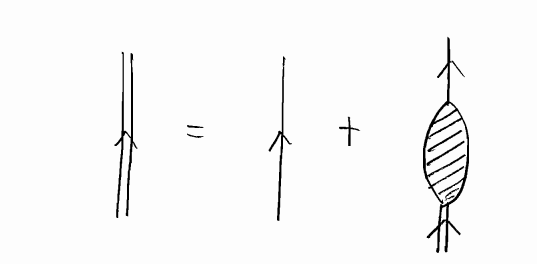
\includegraphics[width = 6cm]{P321.png}
\end{center}
where the lower fermion line is replaced by green's function itself.

Namely, the unknown green's function itself in the left hand side is used for the expression for the green's function, so that the equation becomes a self-consistent equation

This equation is called as Dyson's equation, whose analytic expression is given like this
$$G_{\alpha\beta}(x,y)=G_{\alpha\beta}^0(x,y)+\int \mathrm{d}^4x_1\mathrm{d}^4x_1'G^0_{\alpha\lambda}(x,x_1)\Sigma_{\lambda\mu}^{\star}(x_1,x_1?)G_{\mu\beta}^0(x_1',y)$$
 
By substituting the r.h.s into the left hand side, one can derive this equation out of this.


%323
In the momentum space representation, the Dyson equation become much more simpler. For spatially uniform system, the self-energy can be always Fourier transformed like this

%\begin{align}
\[
\Sigma_{\alpha\beta}^{\star}(x,y) = \frac{1}{(2\pi)^4}\int d^4 k e^{ik(x-y)}\Sigma_{\alpha\beta}^{\star}(k)\]
%\end{align}

With this definition and eq. (2-5-5), the Dyson equation reduces to an algebraic equation: 

\[G_{\alpha\beta}(k) = G^0_{\alpha\beta}(k) + G_{\alpha\lambda}^0(k)\Sigma_{\lambda\mu}^{\star}(k)G_{\mu\beta}(k) \]

For an isotropic system, $G$, $G^0$ and $\Sigma^\star$ becomes diagonal in spin space

\[\begin{split}
G_{\alpha\beta}(k) &= \delta_{\alpha\beta}G(k)\\
G^0_{\alpha\beta}(k) &= \delta_{\alpha\beta}G^0(k)\\
\Sigma^\star_{\alpha\beta}(k) &= \delta_{\alpha\beta}\Sigma^\star_(k)\\
\end{split}\]

As a result, the Dyson equation can be explicitly solved;

\[\begin{split}
&\quad G(k) = G^0(k) + G^0(k)\Sigma^\star(k)G(k)\\
&\Longleftrightarrow (1-G^0(k)\Sigma^\star(k))G(k)=G^0(k)\\
&\Longleftrightarrow G(k) = \frac{1}{{G^0}^{-1}(k)-\Sigma^\star(k)}
\end{split} \]

The inverse of $G^0$ is given by

\[[G^0(k)]^{-1} = \omega - \omega_{\bf k}+i\eta \text{sgn}(|{\bf k}|-k_F) \]

with $\eta\to 0+$

As such, we find

\[G_{\alpha\beta}({\bf k},\omega) = \frac{\delta_{\alpha\beta}}{\omega-\omega_{\bf k}+i\eta\text{sgn}(|{\bf k}|-k_F)}-\Sigma^\star({\bf k},\omega) \]

According to the Lehmann representation, this Green function has a pole above the real axis of $\omega$ when $\omega$ is less than $\mu\hbar$, while it has a pole below the real axis of $\omega$ when $\omega$ is greater than $\mu/\hbar$. 

This general statement ensures the imaginary part of the proper self energy is positive when $\omega$ is less than $\mu/\hbar$, while it is negative otherwise

\[\begin{cases}
\text{Im}\Sigma^\star({\bf k},\omega)\ge 0 &\text{for }\omega\le\mu/\hbar\\
& \\
\text{Re}\Sigma^\star({\bf k},\omega)\le 0 &\text{for }\omega\ge\mu/\hbar
\end{cases}\]

Thanks to this general statement, we can determine the chemical potential in interacting fermion systems as the point at which Im$\Sigma^\star({\bf k},\omega)$ changes the sign. 

In an interacting system, one particle excited state ($a^\dagger_{{\bf k},\lambda}|F.S\rangle (|{\bf k}|>k_F)$) or one-hole excited state ($a_{{\bf k},\lambda}|F.S\rangle (|{\bf k}|<k_F)$) are not an eigenstate of the system, so that these excited particles have a finite life time. Imaginary part of the pole of the Green's function in $\omega<\mu/\hbar$ region describes the life time for the hole, which that in $\omega?\mu/\hbar$ region describes the life time for the particle. 

As an example of the proper self energy, let us consider the first-order \& second-order (Feynman Diagrams)

Within 1st order \& 2nd order, the proper self energies are given like this respectively

\begin{align}
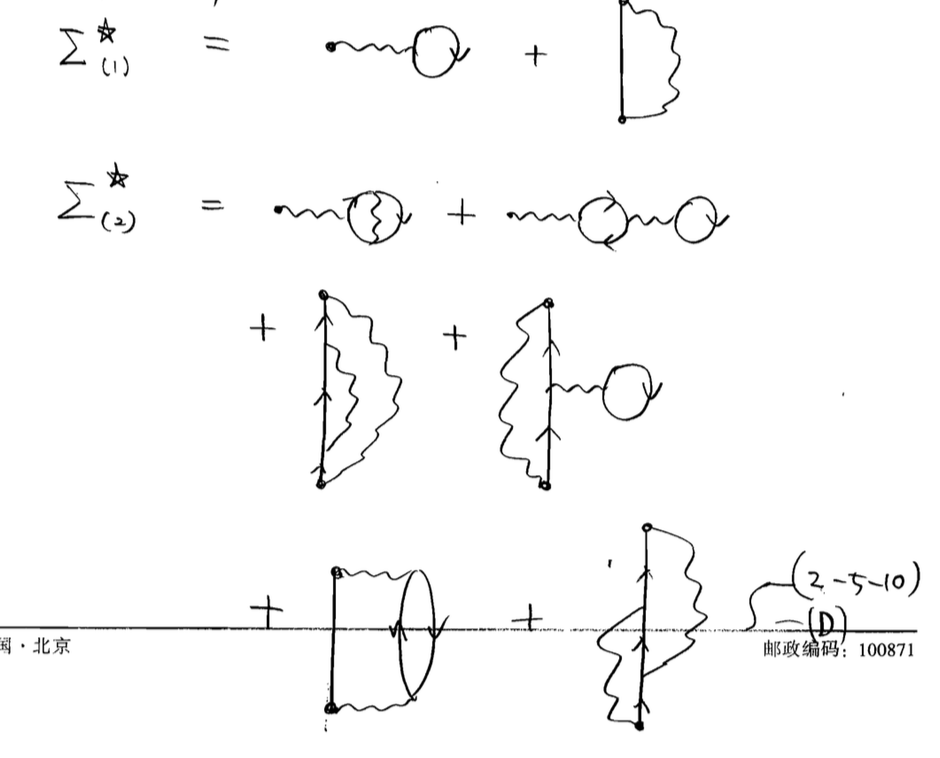
\includegraphics[width = 12cm]{2-5-10D.png}
\end{align}

$\Sigma^\star_{(1)}({\bf k},\omega)$ has been already calculated in eq. (2-5-9):

\[\hbar\Sigma^\star_{(1)} ({\bf k},\omega) = nV_0(0)-\frac{1}{(2\pi)^3}\int d^3{\bf k}'[V_0({\bf k-k}')+3V_1({\bf k-k}')]\theta(k_F-|\bf k|) \]

which does not depend on frequency and which is real valued. 

This means that, within the 1st-order approximation, one-particle state or one-hole state has a infinite life time and effect of the interaction is to change the one-particle spectrum $\omega_{\bf k}$ into another function of $\bf k$

\[\omega_{\bf k}\to\tilde{\omega}_{\bf k} = \omega_{\bf k} + \Sigma^\star_{(1)}({\bf k})=\omega_{\bf k} + \frac{1}{\hbar}nV_0(0) - \frac{1}{\hbar}\int \frac{d{\bf k}'^3}{(2\pi)^3}\times[V_0({\bf k-k}')+3V_1({\bf k-k}')]\theta(k_F-|\bf k'|) \]

Here $nV_0(0)$ is a constant energy shift of the one-particle spectrum, which represents the forward scattering coming from all the other particle. The latter parti represents the exchange scattering. 

Feynman-Dyson perturbation theory developed so far enable us to evaluate the Green's function to all order in the interaction potential. In reality, however, obtaining all order exactly is impossible and we must resort to a certain approximation. As the simplest example, we retained only the first order contribution to the proper self energy. Unfortunately, such an approximation cannot capture the physics of most systems quite well, where inclusions of certain class of higher order terms are necessary. In the following three sections, I will introduce three approximation scheme which goes beyond the 1st-order approximation for the proper self-energy. 

